\documentclass{article}
\usepackage{pgf}
\usepackage{pgfpages}
\usepackage[absolute,overlay]{textpos}

\pgfpagesdeclarelayout{boxed}
{
	\edef\pgfpageoptionborder{0pt}
}
{
	\pgfpagesphysicalpageoptions
	{%
		logical pages=1,%
	}
	\pgfpageslogicalpageoptions{1}
	{
		border code=\pgfsetlinewidth{2pt}\pgfstroke,%
		border shrink=\pgfpageoptionborder,%
		resized width=.95\pgfphysicalwidth,%
		resized height=.95\pgfphysicalheight,%
		center=\pgfpoint{.5\pgfphysicalwidth}{.5\pgfphysicalheight}%
	}%
}

\pgfpagesuselayout{boxed}
\usepackage{amsmath}
\usepackage{graphicx}
\usepackage{geometry}
\usepackage{theorem}
\usepackage{amssymb}
\usepackage{fancyhdr}
\usepackage{extramarks}
\usepackage{amsfonts}
\usepackage{tikz}
\usepackage[plain]{algorithm}
\usepackage{algpseudocode}
\usepackage{url}
\usetikzlibrary{automata,positioning}
\DeclareMathOperator*{\argmax}{argMax}
\usepackage{xepersian}
\settextfont{Yas}
\setlatintextfont{Times New Roman}
\makeatletter
\newcommand*{\Computebaselinestretch}[1]{%
	\strip@pt\dimexpr\number\numexpr\number\dimexpr#1\relax*65536/\number\dimexpr\baselineskip\relax\relax sp\relax
}
\makeatother
\linespread{\Computebaselinestretch{1cm}}

\newtheorem{remark}{ملاحظه}

\topmargin=-0.45in
\evensidemargin=0in
\oddsidemargin=0in
\textwidth=6.5in
\textheight=9.0in
\headsep=0.25in

\linespread{1.5}

\pagestyle{fancy}
\lhead{زمستان ۱۴۰۱}
\chead{}
\rhead{\hmwkClass}
\lfoot{\lastxmark}
\cfoot{\thepage}

\renewcommand\headrulewidth{0.4pt}
\renewcommand\footrulewidth{0.4pt}

\setlength\parindent{0pt}

%
% Create Problem Sections
%

\newcommand{\enterProblemHeader}[1]{
	\nobreak\extramarks{}{تمرین \arabic{#1} در صفحه‌ی بعد ادامه دارد.\ldots}\nobreak{}
	\nobreak\extramarks{تمرین \arabic{#1} (ادامه)}{تمرین \arabic{#1} در صفحه‌ی بعد ادامه دارد.\ldots}\nobreak{}
}

\newcommand{\exitProblemHeader}[1]{
	\nobreak\extramarks{تمرین \arabic{#1} (ادامه)}{تمرین \arabic{#1} در صفحه‌ی بعد ادامه دارد.\ldots}\nobreak{}
	\stepcounter{#1}
	\nobreak\extramarks{تمرین \arabic{#1}}{}\nobreak{}
}

\setcounter{secnumdepth}{0}
\newcounter{partCounter}
\newcounter{homeworkProblemCounter}
\setcounter{homeworkProblemCounter}{1}
\nobreak\extramarks{تمرین \arabic{homeworkProblemCounter}}{}\nobreak{}

%
% Homework Problem Environment
%
% This environment takes an optional argument. When given, it will adjust the
% problem counter. This is useful for when the problems given for your
% assignment aren't sequential. See the last 3 problems of this template for an
% example.
%
\newenvironment{homeworkProblem}[1][-1]{
	\ifnum#1>0
	\setcounter{homeworkProblemCounter}{#1}
	\fi
	\section{{\huge تمرین \arabic{homeworkProblemCounter}}}
	\setcounter{partCounter}{1}
	\enterProblemHeader{homeworkProblemCounter}
}{
	\exitProblemHeader{homeworkProblemCounter}
}

%
% Homework Details
%   - Title
%   - Due date
%   - Class
%   - Section/Time
%   - Instructor
%   - Author
%

\newcommand{\hmwkTitle}{تمرین سری \#۵}
\newcommand{\hmwkDueDate}{}
\newcommand{\hmwkClass}{گزارش اولیه پروژه پایانی درس یادگیری ماشین}
\newcommand{\hmwkClassTime}{دکتر نجاراعرابی}
\newcommand{\hmwkClassTimea}{دکتر ابوالقاسمی دهاقانی}
\newcommand{\hmwkClassTimeb}{دکتر توسلی پور}
\newcommand{\hmwkClassInstructor}{اساتید درس:}
\newcommand{\hmwkAuthorName}{\textbf{بهراد موسایی شیرمحمد ۸۱۰۱۰۱۲۷۸}}
\newcommand{\hmwkAuthorNamea}{\textbf{گردآورندگان: }}
\newcommand{\hmwkAuthorNameb}{\textbf{محمد سجاد علمدار ۸۱۰۱۰۱۲۳۱ }}
\newcommand{\hmwkAuthorNamec}{\textbf{ملیکا فتحی پور ۸۱۰۱۰۰۴۲۴}}
\newcommand{\hmwkAuthorNamed}{\textbf{محمد جواد رنجبر کلهرودی ۸۱۰۱۰۱۱۷۳ }}


%
% Title Page
%

\title{\raisebox{-5mm}[0pt][0pt]{
	
\includegraphics[width=5cm]{/Users/behradmousaie/Desktop/ML_Project/Latex/Photo/eng-logo.png}\hspace*{-20cm} }
	\begin{textblock*}{5cm}(8.2cm,2cm)  
		\textbf{دانشگاه تهران\\
			دانشکده فنی \\
		گروه برق و کامپیوتر}
	\end{textblock*}
\raisebox{-10mm}[0pt][0pt]{
	
\includegraphics[width=5cm]{/Users/behradmousaie/Desktop/ML_Project/Latex/Photo/logo.png}\hspace*{0cm} }\\
	\vspace{1in}
	\textmd{\textbf{\Huge{گزارش اولیه پروژه پایانی یادگیری ماشین}}}\\
	\normalsize\vspace{0.5in}\small{\hmwkDueDate\ }\\
	\vspace{0.5in}\large{\textit{\hmwkClassInstructor\ \\ \hmwkClassTime \\ \hmwkClassTimea \\ \hmwkClassTimeb}}
	\vspace{1.2in}
}

\author{\hmwkAuthorNamea \\ \hmwkAuthorNameb \\ \hmwkAuthorName \\ \hmwkAuthorNamec \\ \hmwkAuthorNamed \\ 
	\begin{textblock*}{5cm}(8.2cm,25cm)  
	\textbf{زمستان ۱۴۰۱}
\end{textblock*}
}
\date{}

\renewcommand{\part}[1]{\textbf{\large Part \Alph{partCounter}}\stepcounter{partCounter}\\}

%
% Various Helper Commands
%

% Useful for algorithms
\newcommand{\alg}[1]{\textsc{\bfseries \footnotesize #1}}

% For derivatives
\newcommand{\deriv}[1]{\frac{\mathrm{d}}{\mathrm{d}x} (#1)}

% For partial derivatives
\newcommand{\pderiv}[2]{\frac{\partial}{\partial #1} (#2)}

% Integral dx
\newcommand{\dx}{\mathrm{d}x}

% Alias for the Solution section header
\newcommand{\solution}{\textbf{\huge پاسخ}}

% Probability commands: Expectation, Variance, Covariance, Bias
\newcommand{\E}{\mathrm{E}}
\newcommand{\Var}{\mathrm{Var}}
\newcommand{\Cov}{\mathrm{Cov}}
\newcommand{\Bias}{\mathrm{Bias}}
\begin{document}
		\large
    	\maketitle
	\pagebreak
	
	\tableofcontents
	\newpage
	
	\listoffigures
	\newpage
\section{۰) پیوست}
تمامی موارد خواسته شده در پروژه به طور کامل درون فایل notebook است همچنین تمامی موارد خواسته شده در گزارش توضیه داده شده اما برای جلوگیری از طولانی شدن تعدادی محدود از جدول ها و شکل ها برای تحلیل آورده شده است.
\section{۱) مقدمه}

در این پروژه قصد داریم مدل‌هایی برای تشخیص دستگاه موسیقی ایرانی پیاده سازی کنیم.  این مدل‌ها با استفاده از الگوریتم‌های یادگیری ماشین این دستگاه‌ها را طبقه‌بندی و خوشه‌بندی می‌کنند. برای این منظور مراحل مختلفی را باید طی کنیم تا داده‌ها را آماده برای انجام این کار کنیم. خلاصه‌ای از مراحل در ادامه توضیح داده شده است:  \newline
\textbf{جمع آوری داده:} 
\newline
ابتدا باید مجموعه داده‌ای \footnote{Dataset} برای این کار آماده کنیم، این مجموعه داده توسط دانشجویان دانشگاه تهران به روش جمع‌سپاری \footnote{Crowdsourcing} شده است. این داده‌ها به  فرمت mp3 در 7 کلاس شور، سه‌گاه، ماهور، همایون، راست‌پنج‌گاه، نوا و چهارگاه هستند. طول این قطعات موسیقی بین 20 تا 600 ثانیه می‌باشد. همینطور، ساز‌هایی که این قطعات در آن‌ها نواخته شده‌اند نیز در داخل این مجموعه داده مشخص شده است.\newline
\textbf{استخراج ویژگی:} \newline
موسیقی نمونه‌ای از سیگنال صوتی می‌باشد که ویژگی‌های مخصوص خود را دارا می‌باشد. ما برای آموزش مدل مناسب که قابلیت تعمیم‌پذیری داشته باشد باید، ویژگی‌هایی که در مشخص کردن دستگاه موسیقی اثر دارد را پیدا کرده و استخراج کنیم.\newline
\textbf{مصور‌سازی و تمیز کردن داده‌ها:} \newline
برای اینکه مدلی مناسب برای این کار درست کنیم، بسیار اهمیت دارد که داده‌های آموزش کمترین مقدار خطا را داشته باشد تا از آموزش داده شدن مدل با داده‌های نویزی\footnote{Noise} جلوگیری کنیم. بدین منظور بایست ابتدا داده‌ها را بر اساس ویژگی‌ها مصور‌سازی کرده تا هم در صورت وجود داده‌های نادرست آن‌ها را بیابیم و حذف کنیم و همینطور با بررسی الگوهای داده بهترین مدل را برای وظیفه طبقه‌بندی انتخاب کنیم. همچنین، در صورت نیاز می‌توان داده‌های موسیقی را به چندین داده با طول کمتر تبدیل کرد تا مجموعه داده‌ای با تعداد داده‌ی بیشتر دست یابیم.\newline
\textbf{مصور‌سازی و تمیز کردن داده‌ها طبقه‌بندی:} \newline
حال پس از تمیز کردن داده‌ و استخراج ویژگی‌های آن، می‌توانیم بر اساس اطلاعات به دست آمده از گام قبلی مدل‌هایی طراحی کنیم که بهترین عملکرد را برای داده‌ی ما بدهند. در این پروژه از مدل‌های طبقه‌بند مانند SVM ،  شبکه عصبی چند لایه\footnote{Multilayer perceptron} و XGBoost برای این کار استفاده می‌کنیم.\newline
\textbf{خوشه بندی:} \newline
در این مرحله نیز با استفاده از روش‌های خوشه‌بندی و اطلاعات به دست آمده در گام‌های قبلی، سعی در جداسازی داده‌ها خواهیم کرد. در این پروژه از دو مدل Kmeans و Agglomerative برای جداسازی داده‌ها استفاده خواهد شد.\newline
در ادامه تمامی مراحل بالا را به صورت کامل پیاده‌سازی کرده و توضیح می‌دهیم.
\newpage

\section{۲) ویژگی‌های موسیقی}
\subsection{۲-۱) موسیقی چیست؟}
موسیقی یک  نمونه از سیگنال صوتی می‌باشد و در نتیجه تمامی ویژگی‌ها مربوط به یک سیگنال را دارا است. و به عبارتی همین ویژگی‌ها هستند که تفاوت را در قطعه‌های موسیقی ایجاد می کند.
\newline
به طور کلی سیگنال‌ها داری سه ویژگی معروف و مهم هستند که به شرح زیر مطرح می‌شوند:\newline
۱) دامنه:
مشخص کننده این که چه مقدار سیگنال قوی و ضعیف هست.\newline
۲) فرکانس:
به صورت ساده شده می‌توان گف، تعداد دفعاتی که در واحد زمان، موج سیگنال تکرار می‌شود را فرکانس می‌گوییم. در سیگنال صوتی هر چقدر فرکانس افزایش یابد صدا زیرتر می‌شود و هرچقدر فرکانس کاهش یابد صدا بم‌تر می شود.\newline
۳) فاز:
زاویه اولیه سیگنال در نقطه مبدا است. ( البته نسبت به دو مورد دیگر کاربرد کمتری در بحث ما دارد.)\newline
\begin{figure}[h]
	\centering
	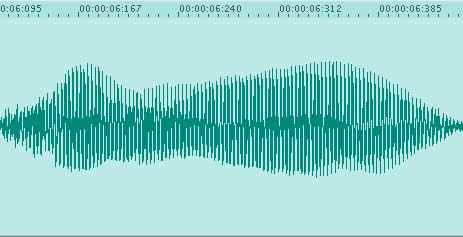
\includegraphics[width=0.5\linewidth]{Photo/1}
	\caption[شمای کلی سیگنال موسیقی]{شمای کلی سیگنال موسیقی}
	\label{fig:1}
\end{figure}

\subsection{۲-۲) فرمت های صوتی}
فایل‌های صوتی دیجیتال با فرمت wav. امواج صوتی هستند که با نمونه‌برداری از موسیقی آنالوگ در فواصل گسسته دیجیتالی می‌شوند. (معمولاً 44.1 کیلوهرتز برای صدای با کیفیت CD به این معنی که نمونه‌ها 44100 بار در ثانیه گرفته می شوند). هر نمونه، برابر با مقدار دامنه  سیگنال در یک بازه زمانی خاص است. نکته اصلی در مورد فرمت wav این است که یک فرمت بدون فشرده‌سازی یا Uncompressed است. به همین سبب کیفیت بالا و اصلی موسیقی آنالوگ را حفظ می‌کند ولی در مقابل حجم آن بسیار زیاد است. همچنین از ان جهت که این فرمت به صورت ۳۲ بیت بدون علامت تعریف می‌شود حداکثر تا ۴ گیگابیت می‌تواند حجم داشته باشد بنابراین مدت زمان ضبط موسیقی با این فرمت، نسبت به فرمت‌های فشرده مثل  \lr{MP3} و \lr{MP4} و \lr{OGG} محدود تر است.\newline
در این پروژه فایل های صوتی به صورت \lr{MP3} تهیه شدند که در مورد این فرمت صوتی می‌توان گفت که یک فرمت رمزگذاری داده‌های صوتی دیجیتالی است که با استفاده از روش "اتلاف (حذف) داده‌ها" (Lossy data) این داده‌های صوتی را فشرده می‌کند؛ یعنی فرمت \lr{MP3} قسمت‌های خاصی از فایل صوتی اصلی را از بین می‌برد و سایر قسمت‌ها را فشرده می‌کند. اعمال کلی که در پروسه فشرده‌سازی فایل صوتی توسط فرمت \lr{MP3} انجام می‌شود، عبارت‌اند از:\newline
- حذف قسمت‌هایی از فایل صوتی که خارج از محدوده شنیداری گوش انسان است.\newline
- حفظ لایه‌های صوتی‌ای که گوش انسان بهتر از سایر لایه‌های صوتی می‌شوند.\newline
- حذف لایه‌های صوتی کوتاه تر که به صورت همزمان با لایه‌های صوتی بلندتر پخش می‌شوند.\newline
لازم به ذکر است که کتابخانه‌های معروف کار با صوت در پایتون\footnote{Python} معمولا با فایل‌های wav کار می‌کنند لذا در این پروژه نیاز به تبدیل این فایل‌های mp3 به این فرمت داشتیم.
\subsection{۲-۳) سیگنال صوتی}
باتوجه به مطالب بالا به طورکلی می توان به این نتیجه رسید که موسیقی به شکل یک سیگنال صوتی با پارامترهایی مانند فرکانس، پهنای باند و غیره نمایش داده می شود. یک سیگنال صوتی معمولی را می‌توان به عنوان تابعی از دامنه و زمان نشان داد که در شکل زیر مشخص است.
\begin{figure}[h]
	\centering
	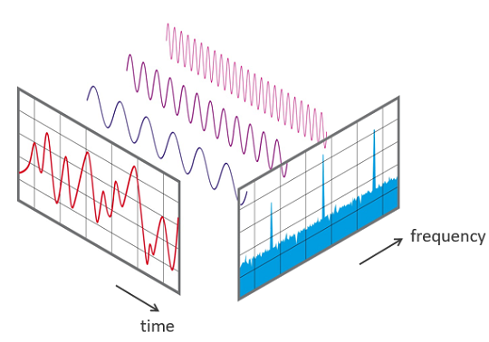
\includegraphics[width=0.5\linewidth]{Photo/2}
	\caption[نمایش یک سیگنال صوتی]{نمایش یک سیگنال صوتی}
	\label{fig:2}
\end{figure}

معمولا این سیگنال‌های صوتی به فورمت‌های \lr{wav (Waveform Audio File)}  ، \lr{mp3 (MPEG-1 Audio Layer 3)} و  \lr{WMA (Windows Media Audio)}به صورت دیجتالی موجود هستند. به عنوان مثال نمونه‌ای از سیگنال یک موسیقی در دو دستگاه نوا و شور را در ادامه مشاهده می‌کنید:
\begin{figure}[h]
	\centering
	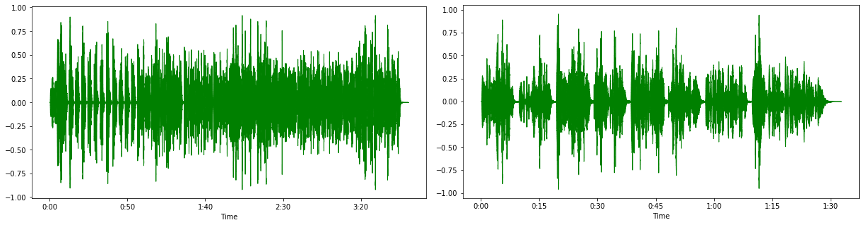
\includegraphics[width=0.7\linewidth]{Photo/3}
	\caption[نمونه‌ای از سیگنال موسیقی در دستگاه نوا و شور]{نمونه‌ای از سیگنال موسیقی در دستگاه نوا و شور}
	\label{fig:3}
\end{figure}
حال با توجه به اطلاعاتی که مورد سیگنال‌های صوتی به دست آوردیم به بررسی ویژگی‌های اصلی و مورد استفاده در پروژه می‌پردازیم.
\subsection{۲-۴) ویژگی‌های حوزه زمان}
نرخ عبور از صفر \lr{(Zero crossing rate)}: \newline
نرخ عبور از صفر (ZCR) در یک سیگنال به معنی تعداد دفعاتی است که سیگنال از مثبت به صفر و به منفی یا از منفی به صفر و به مثبت تغییر می کند. یا به عبارت دیگر نرخ تغییر علامت سیگنال است. این ویژگی را می‌توان به صورت زیر نیز فرموله کرد: 
\begin{equation}
	ZCR=\dfrac{1}{T - 1} \cdot \sum_{i=1}^{T-1} 1_{R_{<0}}\cdot(s_{t} \cdot s_{t-1})
\end{equation}
که S را در معادله بالا به صورت سیگنالی به طول T در نظر بگیریم و در ادامه  $ 1_{R_{<0}} $ نیز تابعی برای مقادیر زیر صفر قابل برداشت خواهد بود.\newline
\begin{figure}[h]
	\centering
	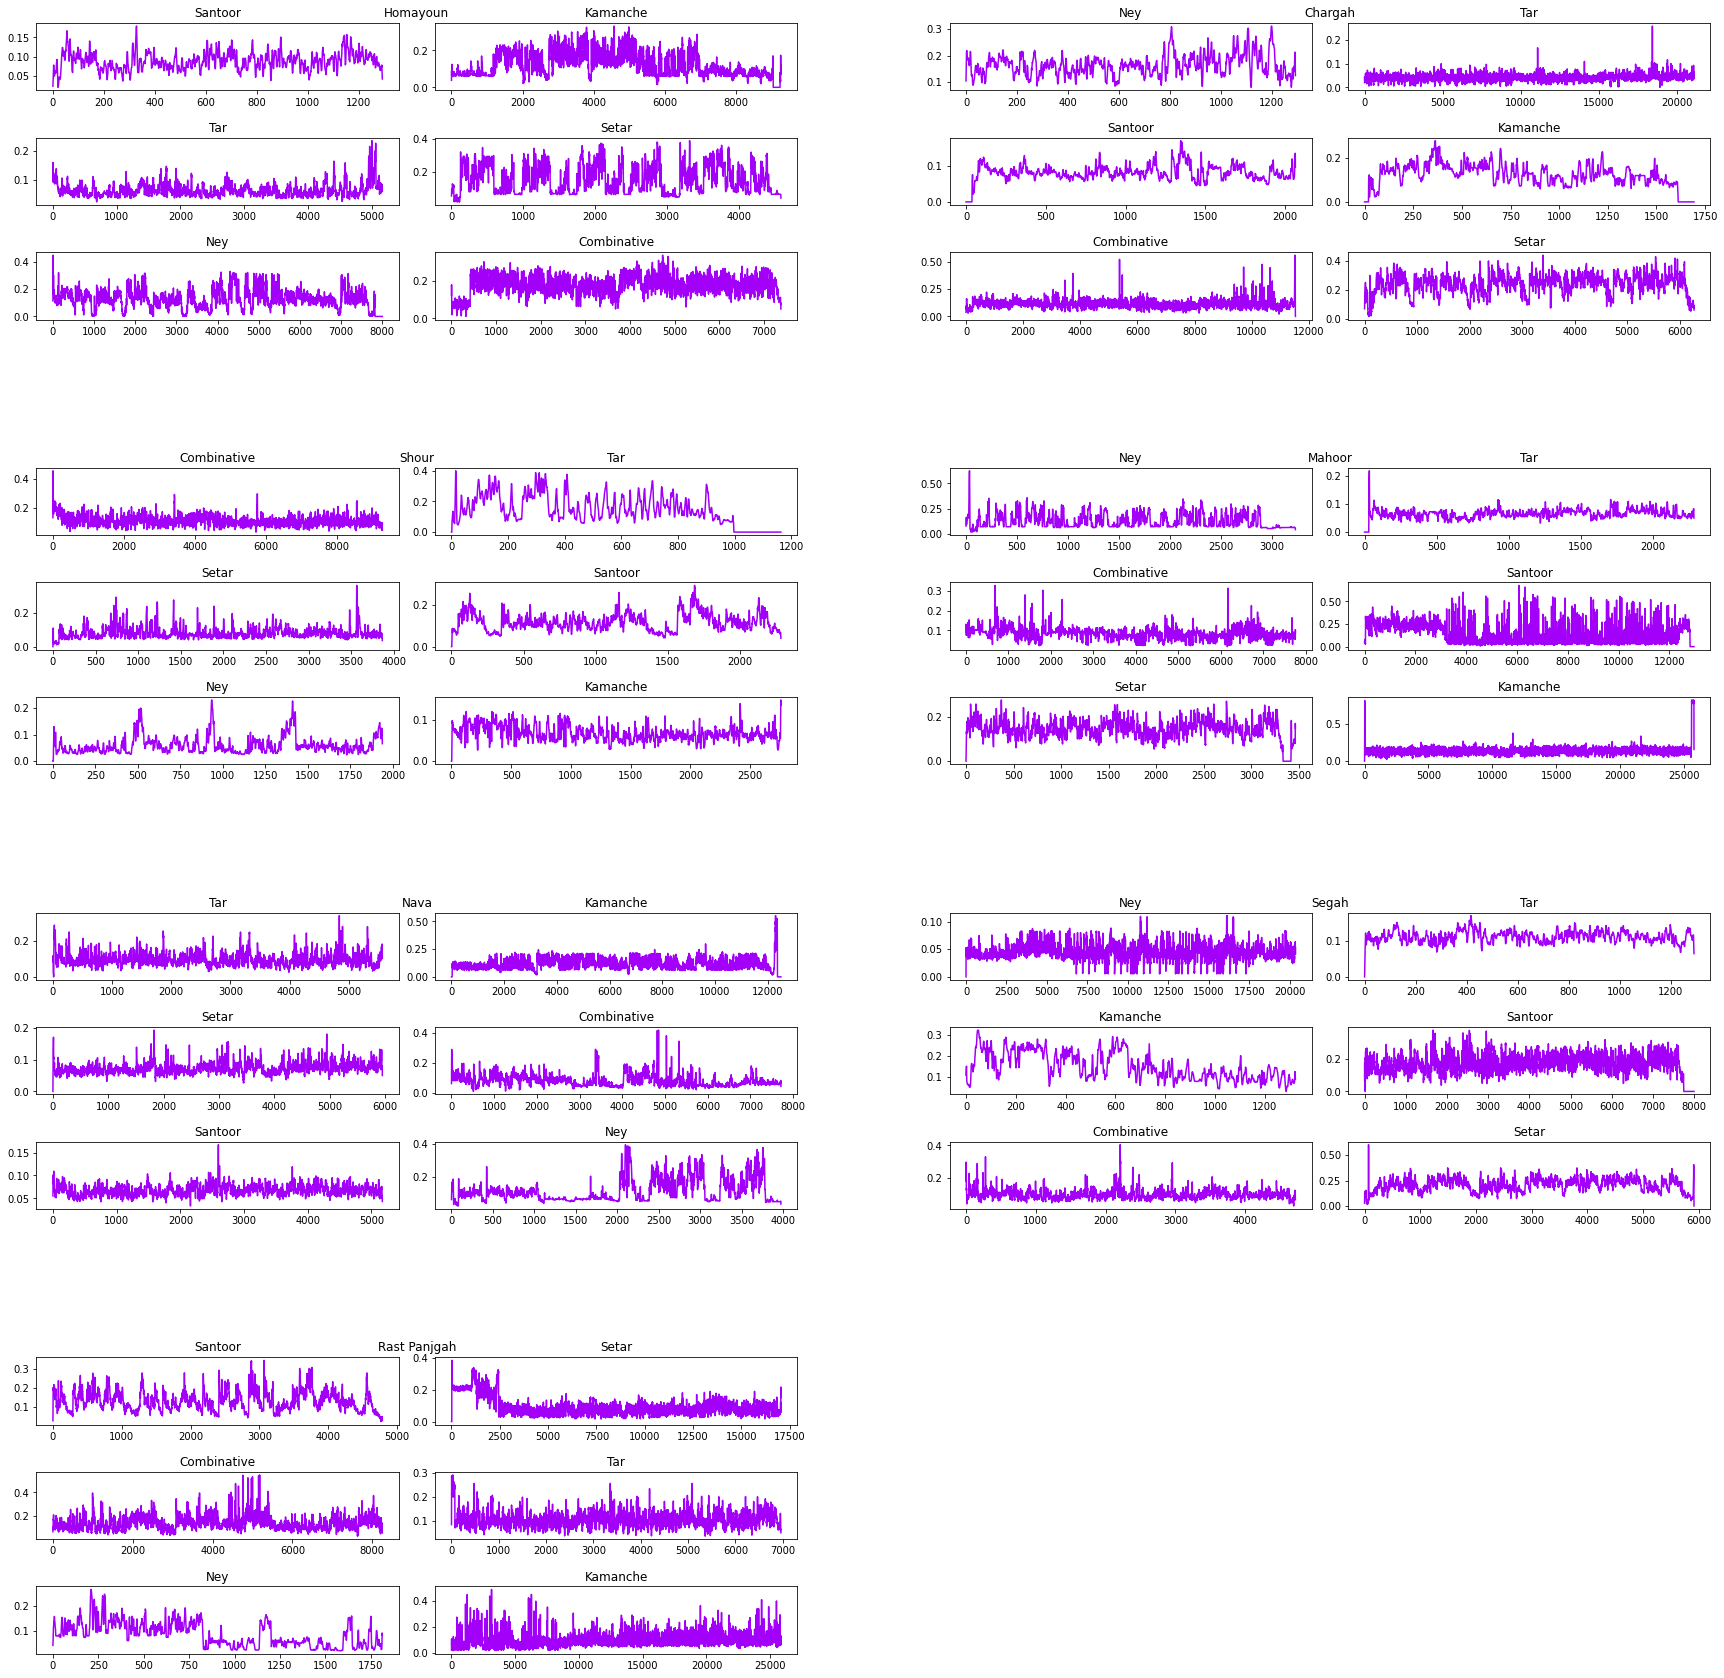
\includegraphics[width=0.5\linewidth]{Photo/Zero_crossing}
	\caption[نرخ گذر از صفر]{نرخ گذر از صفر}
	\label{fig:24}
\end{figure}
در شکل نرخ گذر از صفر برای نمونه‌های مختلف از موسیقی‌های در کلاس‌های مختلف نشان داده شده است.

جذر میانگین مربعات انرژی \lr{root-mean-square energy (RMSE)}: \newline
انرژی در سیگنال‌های صوتی به صورت ساده شده برابر با اندازه‌ی سیگنال است. به عبارتی دیگر می‌توان گفت که انرژی تقریبا برابر به این است که چقدر یک صوت بلند است. جذر میانگین مربعات انرژی از رابطه زیر بدست می‌آید:
\begin{equation}
	RMSE = \sqrt{\dfrac{1}{N}\cdot \sum_{n}^{} |x(n)|}
\end{equation}
آنتروپی شانون \lr{ (Shannon entropy)}:  \newline
آنتروپی کلاسیک شانون اطلاعات ارائه شده توسط مجموعه ای از رویدادها را اندازه گیری می‌کند و عدم قطعیت آن را نشان می‌دهد:
\begin{equation}
	H(x) = - \sum_{i=1}^{n}p(x_{i})\cdot log_{b}p(x_{i})
\end{equation}
\subsection{۲-۵) ویژگی‌های حوزه فرکانس}
اندازه طیف سیگنال:\newline
نشان دهنده ميزان انرژي در حوزه فركانس است، به عبارت ديگر مي‌توان از این مقدار متوجه شد كه در هر فركانس خاص، چه ميزان انرژي وجود دارد. تبدیل فوریه زمان-کوتاه \footnote{Short-time Fourier transform} در اين تبديل سيگنال حوزه زمان را به پنجره‌های \footnote{Frame} كوتاه مدت تقسيم مي کند و از هر فريم تبديل فوريه مي‌گیرد. \newline
به صورت کلی، بسیاری از سیگنال‌هایی که در کاربردهای عملی با آن ها مواجه هستیم به صورتی هستند که تغییرات آن‌ها در طول زمان را نمی‌توان به صورت دقیق توصیف کرد. در مورد این سیگنال‌ها فقط می‌توان عباراتی احتمالاتی برای توصیف تغییرات به کار برد. ابزار ریاضی برای مطالعه این سیگنال‌ها، همان ابزاری است که برای توصیف «دنباله‌های تصادفی» (Random Sequence) مورد استفاده قرار می‌گیرد که متشکل از گروهی از «تحقق‌های» (Realizations) محتمل است که هر کدام دارای احتمال وقوع مختص به خود هستند. واضح است که از کل گروه تحقق، هر «آزمایش کننده» (Experimenter) فقط یکی از تحقق‌های سیگنال را مشاهده\footnote{Observe}  می‌کند.\newline
البته شایان ذکر است که ممکن است به این صورت تصور شود که می‌توان یک تعریف «قطعی» (Deterministic) را برای توصیف این سیگنال‌ها نیز مورد استفاده قرار داد. اما این تصور غلط است؛ زیرا تحقق یک سیگنال تصادفی به صورت یک دنباله گسسته با زمان دیده می‌شود که انرژی محدود ندارد و به همین دلیل نمی‌توان از تبدیل فوریه گسسته با زمان یا DTFT در مورد آن‌ها استفاده کرد. یک سیگنال تصادفی همواره دارای توان متوسط محدود است و بنابراین می‌توان با یک چگالی طیف توان میانگین آن‌ها را توصیف کرد. برای سادگی در ادامه به این مقدار فقط با نام چگالی طیف توان اشاره خواهیم کرد.\newline
براي مشاهده بهتره اسپكتروگرام يك موسيقي در شكل زير به همراه RMS رسم شده است.
\begin{figure}[h]
	\centering
	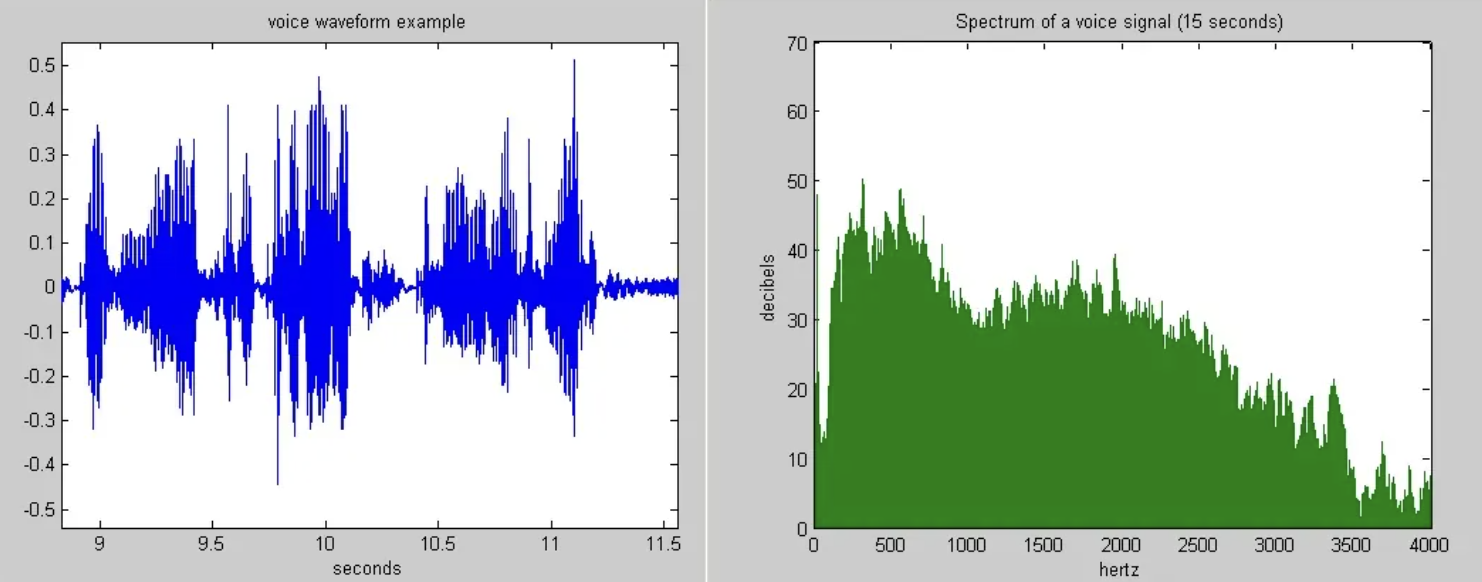
\includegraphics[width=0.7\linewidth]{Photo/4}
	\caption[اسپکتروگرام یک موسیقی]{اسپکتروگرام یک موسیقی}
	\label{fig:4}
\end{figure}\newline
\lr{STFT(Short-time Fourier transform)}:\newline
تبدیل فوریه کوتاه مدت (STFT)، یک تبدیل مرتبط با فوریه است که برای تعیین فرکانس سینوسی و محتوای فاز بخش‌های محلی سیگنال در طول زمان تغییر می‌کند. در عمل، روش محاسبه STFT ها به این صورت است که سیگنال زمان طولانی تری را به بخش های کوتاه تر با طول مساوی تقسیم می کند و سپس تبدیل فوریه را به طور جداگانه در هر بخش کوتاه تر محاسبه می کند. این طیف فوریه را در هر بخش کوتاه تر نشان می دهد. \newline
سپس معمولاً یک طیف متغیر را به عنوان تابعی از زمان رسم می‌کند، که به عنوان طیف‌نگار یا نمودار آبشار شناخته می‌شود، مثلاً ,معمولاً در نمایش‌های طیف مبتنی بر رادیو , نرم‌افزار (SDR) استفاده می‌شود. نمایشگرهای با پهنای باند کامل که کل محدوده یک SDR را پوشش می‌دهند.\newline
\begin{figure}[h]
	\centering
	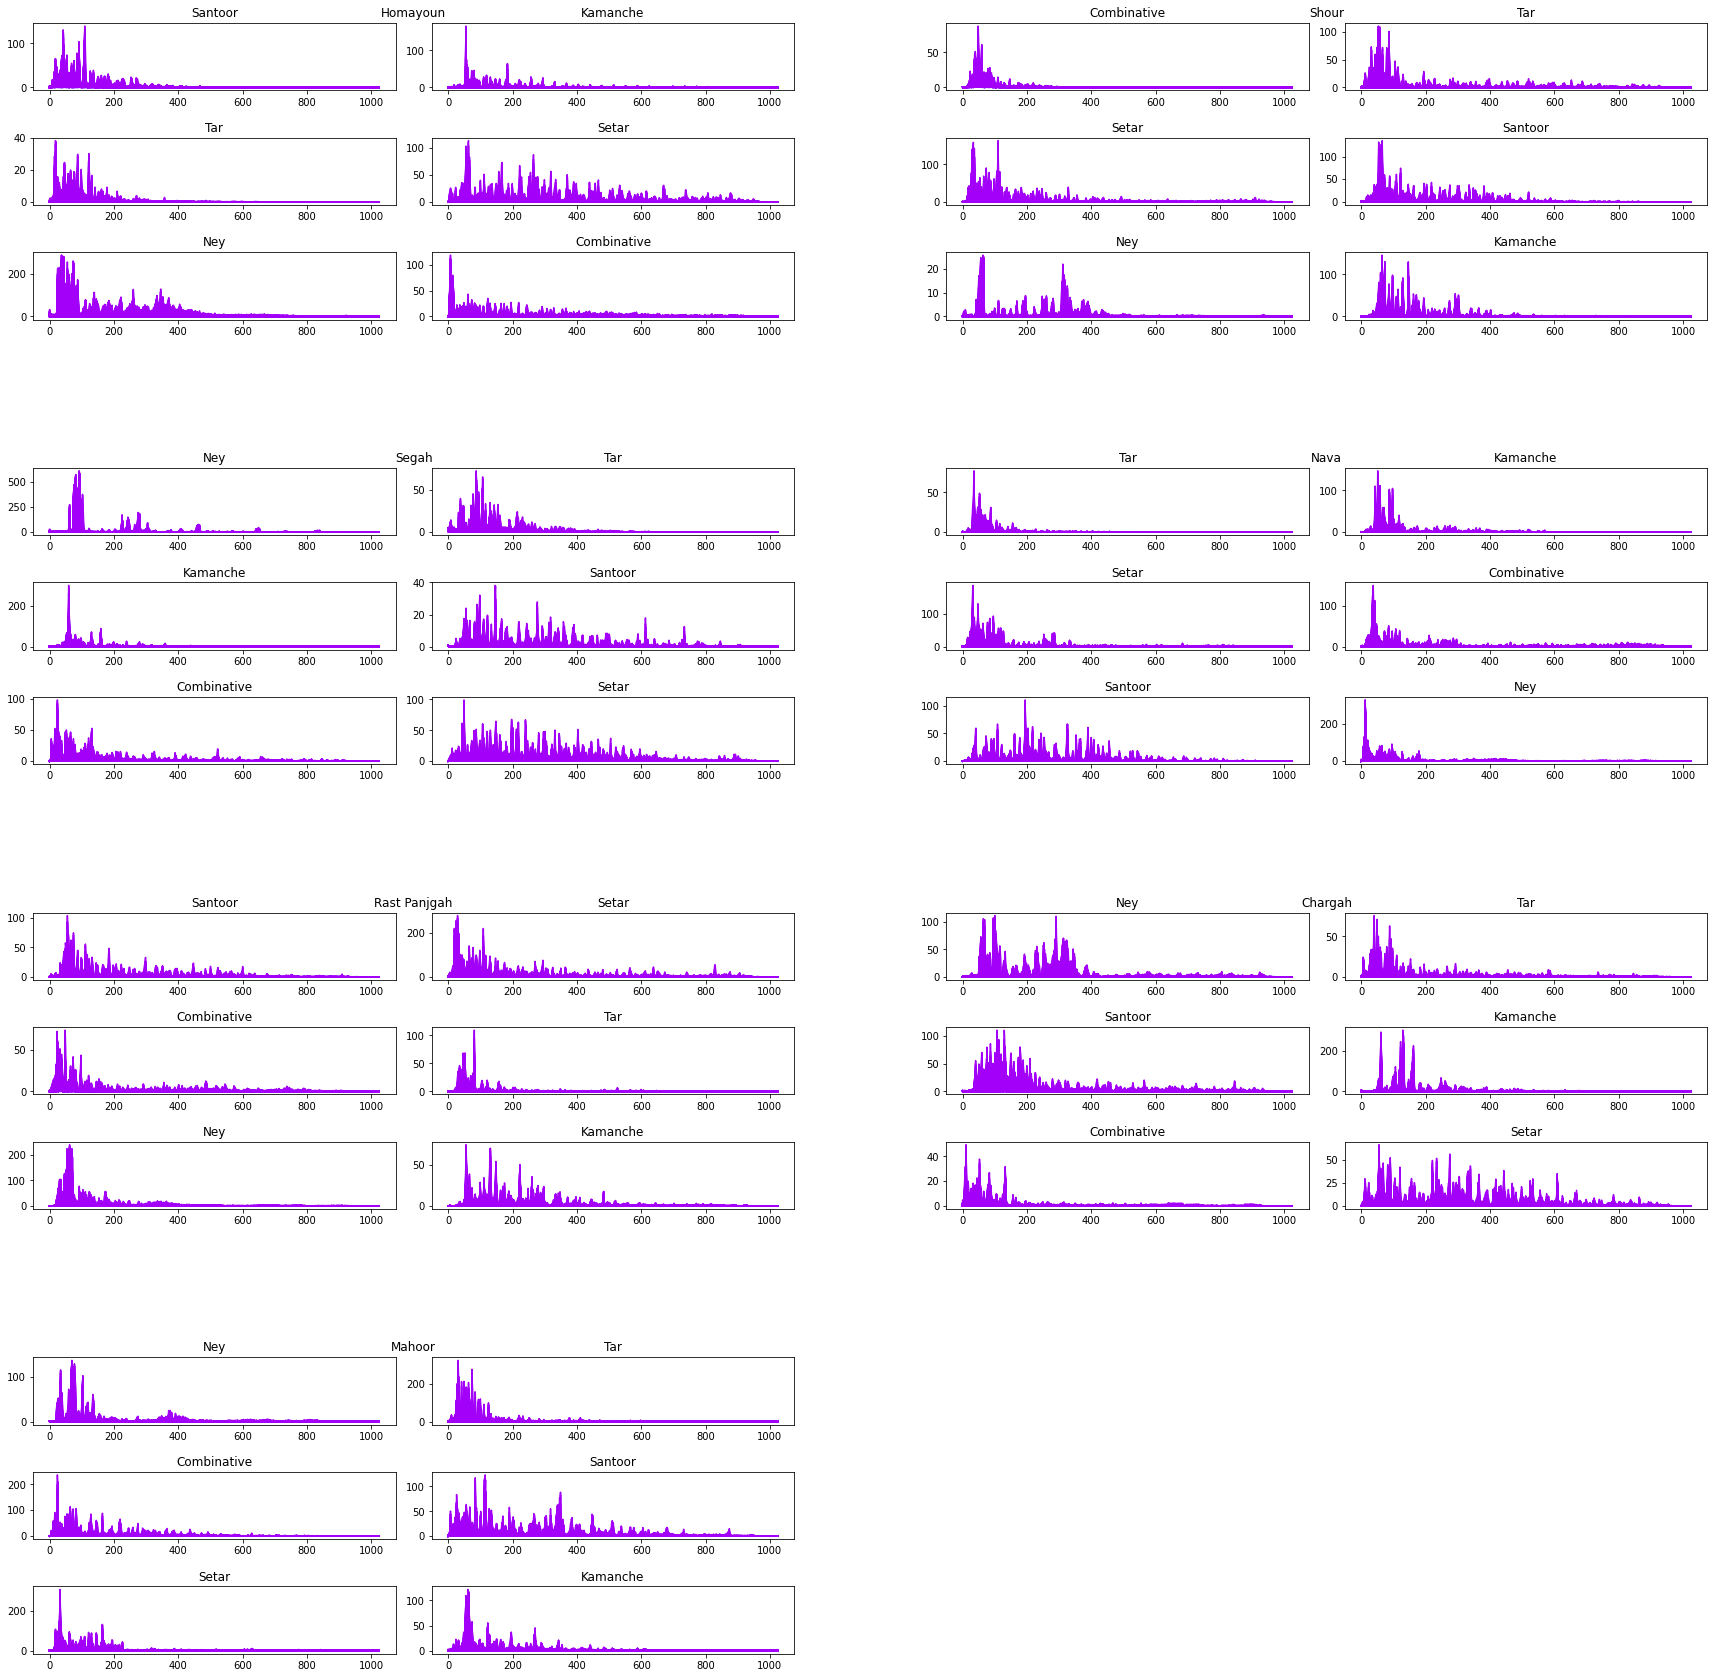
\includegraphics[width=0.5\linewidth]{Photo/25}
	\caption[نمونه ای از \lr{SFTF}]{نمونه ای از \lr{SFTF}}
	\label{fig:25}
\end{figure}

\lr{Continuous-time STFT}:\newline
به سادگی، در حالت زمان پیوسته، تابعی که باید تبدیل شود در یک تابع پنجره که فقط برای مدت کوتاهی غیر صفر است ضرب می شود. تبدیل فوریه (یک تابع یک بعدی) سیگنال حاصل گرفته می‌شود، سپس پنجره در امتداد محور زمان لغزش می‌یابد تا انتها منجر به نمایش دو بعدی سیگنال شود. از نظر ریاضی به صورت زیر نوشته می شود:
\begin{equation}
	STFT{x(t)}(\tau , \omega)=X(\tau , \omega)=\int_{-\infty}^{\infty} x(t)\cdot \omega(t- \tau)\cdot \exp^{-it\omega}\cdot dt
\end{equation}
در معادله بالا $\omega$ تابع پنجره است و همچنین x سیگنال در حال تبدبل است و همان طور که مشخص است X تبدیل فوریه x$\omega$ است.\newline


\lr{Discrete-time STFT}:\newline
در مورد زمان گسسته، داده‌هایی که باید تبدیل شوند را می‌توان به تکه‌ها یا فریم‌هایی تقسیم کرد (که معمولاً روی یکدیگر همپوشانی دارند، تا مصنوعات در مرز کاهش یابد). هر تکه تبدیل فوریه می شود و نتیجه مختلط به ماتریسی اضافه می شود که بزرگی و فاز را برای هر نقطه در زمان و فرکانس ثبت می کند. این را می توان به صورت زیر بیان کرد:
\begin{equation}
		STFT{x[n]}(m , \omega)=X(m , \omega)=\sum_{-\infty}^{\infty} x[n]\cdot \omega[n-m]\cdot \exp^{-in\omega}
\end{equation}
که همانند گذشته تابع $\omega$ تابع پنجره و x سیگنال در حال تبدیل ولی این بار به صورت گسسته است.\newline
حال با توجه به اطلاعاتی که به دست آوردیم به موضوع اولبه خود بر می گردیم.\newline
قدرمطلق مجذور STFT طیف‌گرام چگالی طیفی توان تابع را به دست می‌دهد:
\begin{equation}
	sepectrogram(x(t))(\tau , \omega)=|X(\tau,\omega)|^{2}
\end{equation}
\begin{figure}[h]
	\centering
	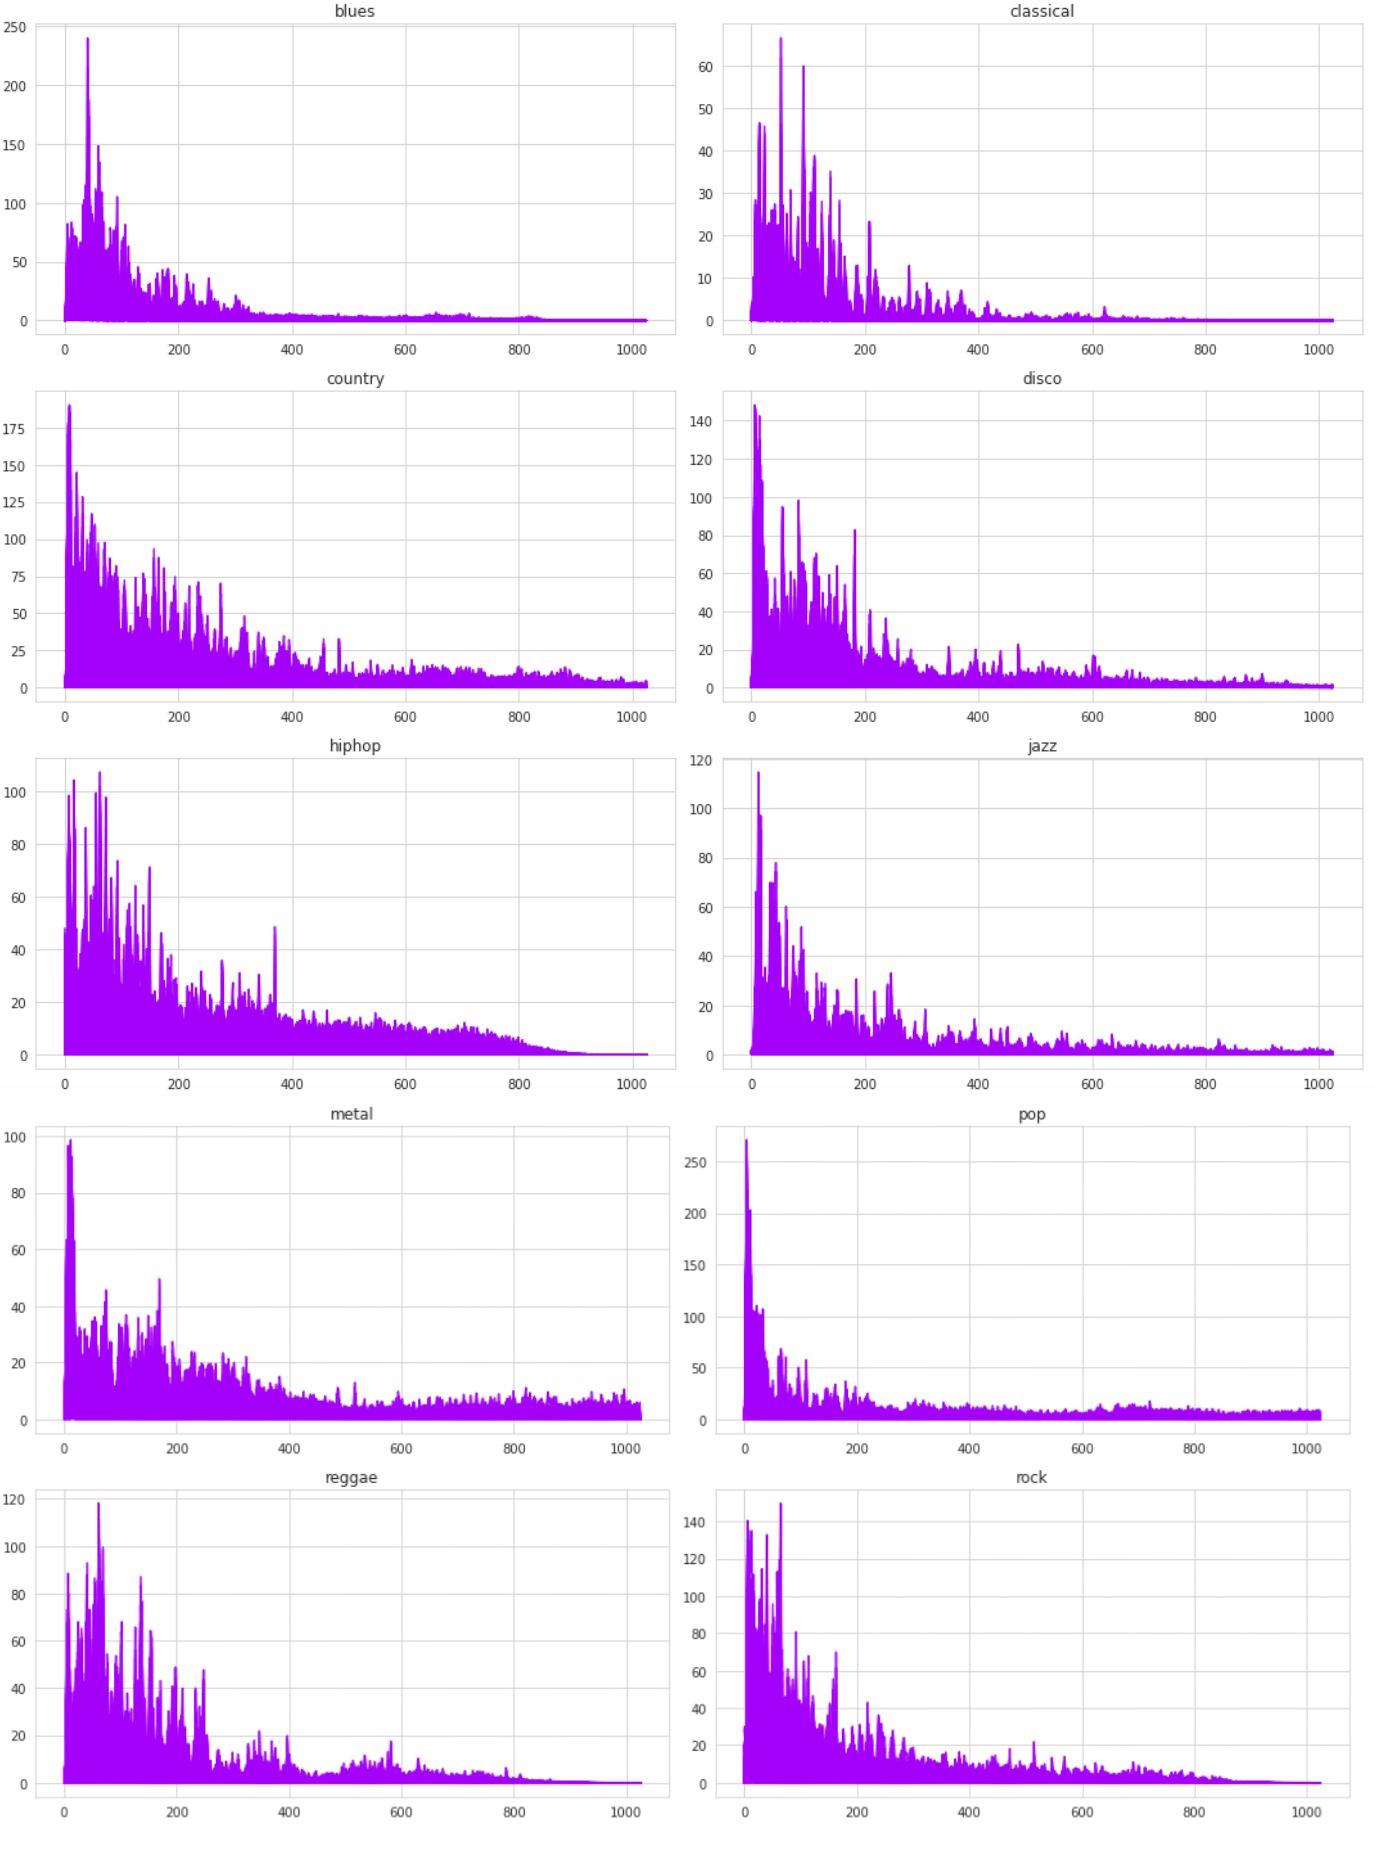
\includegraphics[width=0.5\linewidth]{Photo/5}
	\caption[نمودارهای فرکانس-شدت]{نمودارهای فرکانس-شدت}
	\label{fig:5}
\end{figure}


\lr{Chroma SFTF}: \newline
همان طوز که در شکل زیر نیز قابل مشاهده است, در این بخش از تبدیل فوریه کوتاه مدت که پیشتر به آن اشاره کردیم برای محاسبه ویژگی های chroma استفاده می شود.\newline
در ادمه  STFT اطلاعات مربوط به طبقه بندی پیچ و ساختار سیگنال را نشان می دهد.این نشان را با مقادیر پایین (همانطور که از شبکه نوار رنگ تا نمودار مشخص است) در مقادیر کم (مناطق تاریک) نشان داده می شود.
\begin{figure}[h]
	\centering
	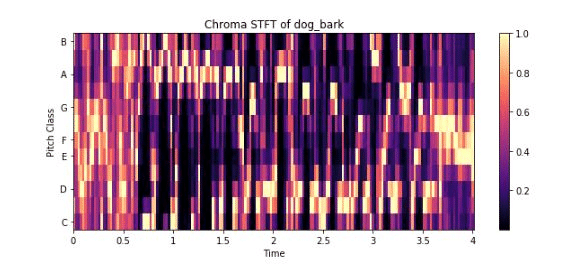
\includegraphics[width=0.7\linewidth]{Photo/7}
	\caption[ویژگی های کروما]{ویژگی های کروما }
	\label{fig:7}
\end{figure}


ویژگی‌های حوزه کپسترال: \newline
یکی از ویژگی هایی که از سیگنال صوتی استخراج می شود و در بسیاری از کاربردها مورد استفاده قرار می گیرد ضرایب کاپسترال می باشند.\newline
آنالیز کپسترال \lr{Capstral Analysis} روشی است متداول در حوزه پردازش سیگنال و پردازش گفتار صوتی به منظور فشرده سازی یا کد کردن گفتار با کیفیت بالا در نرخ بیت \lr{Bit rate} پایین.این روش به طور گسترده ای برای کد نمودن گفتار, سنتز گفتار, شناخت گفتار, شناخت گوینده, احراز هویت گوینده و ذخیره سازی گفتار استفاده می شود.\newline
این ضرایب نه تنها اطلاعات فیلتر مجرای گفتار را در خود دارند, بلکه حاوی اطلاعات سیگنال تحریک نیز هستندو بنابراین مشخصه مناسبی برای گفتار, دسته بندی اصوات و ... می باشند.\newline
از جمله مهمترین انواع آنالیز کپسترال می توان از موارد ذیل نام برد:\newline
\lr{Complex cepstrum} \newline
\lr{Real cepstrum} \newline
\lr{Power cepstrum} \newline
\lr{Phase cepstrum} \newline
اساس کلی آنالیز کپستروم طی کردن روند زیر است:
\begin{figure}[h]
	\centering
	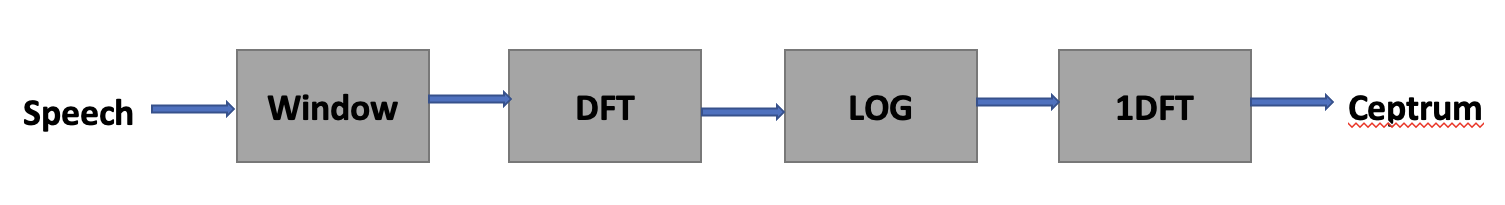
\includegraphics[width=0.7\linewidth]{Photo/6}
	\caption[مراحل آنالیز کپستروم]{مراحل آنالیز کپستروم}
	\label{fig:6}
\end{figure}
اما تفاوت انواع کپستروم در مرحله لگاریتم گیری اتفاق می افتد.به عنوان مثال برای محاسبه \lr{Power ceptrum} از لگاریتم اندازه به توان دو استفاده می کنیم, در محاسبه \lr{Real ceptrum} از اندازه قسمت حقیقی DFT لگاریتم گرفته می شود و ...\newline
تفاوت کپستروم حقیقی و مختلط این است که آنالیز کپستروم مختلط, حاوی اطلاعات فاز سیگنال صحبت نیز هست. اما از آنجا که اطلاعات فاز در شنوایی انسان اهمیت اندکی دارد معمولا از آنالیز کپستروم حقیقی استفاده می شود.\newline

\lr{Harmonics and Perceptrual}:\newline
هارمونیک موج یا سیگنالی است که فرکانس آن مضرب انتگرال (عدد کامل) فرکانس همان سیگنال یا موج مرجع است. به عنوان بخشی از سری هارمونیک، این اصطلاح همچنین می تواند به نسبت فرکانس چنین سیگنال یا موجی به فرکانس سیگنال یا موج مرجع اشاره کند.\newline
در مورد \lr{Perceptrual} می توان گفت که مربوط به احساسات و عاطفه می باشد که به صورت شهودی قابل بیان است.
\begin{figure}[h]
	\centering
	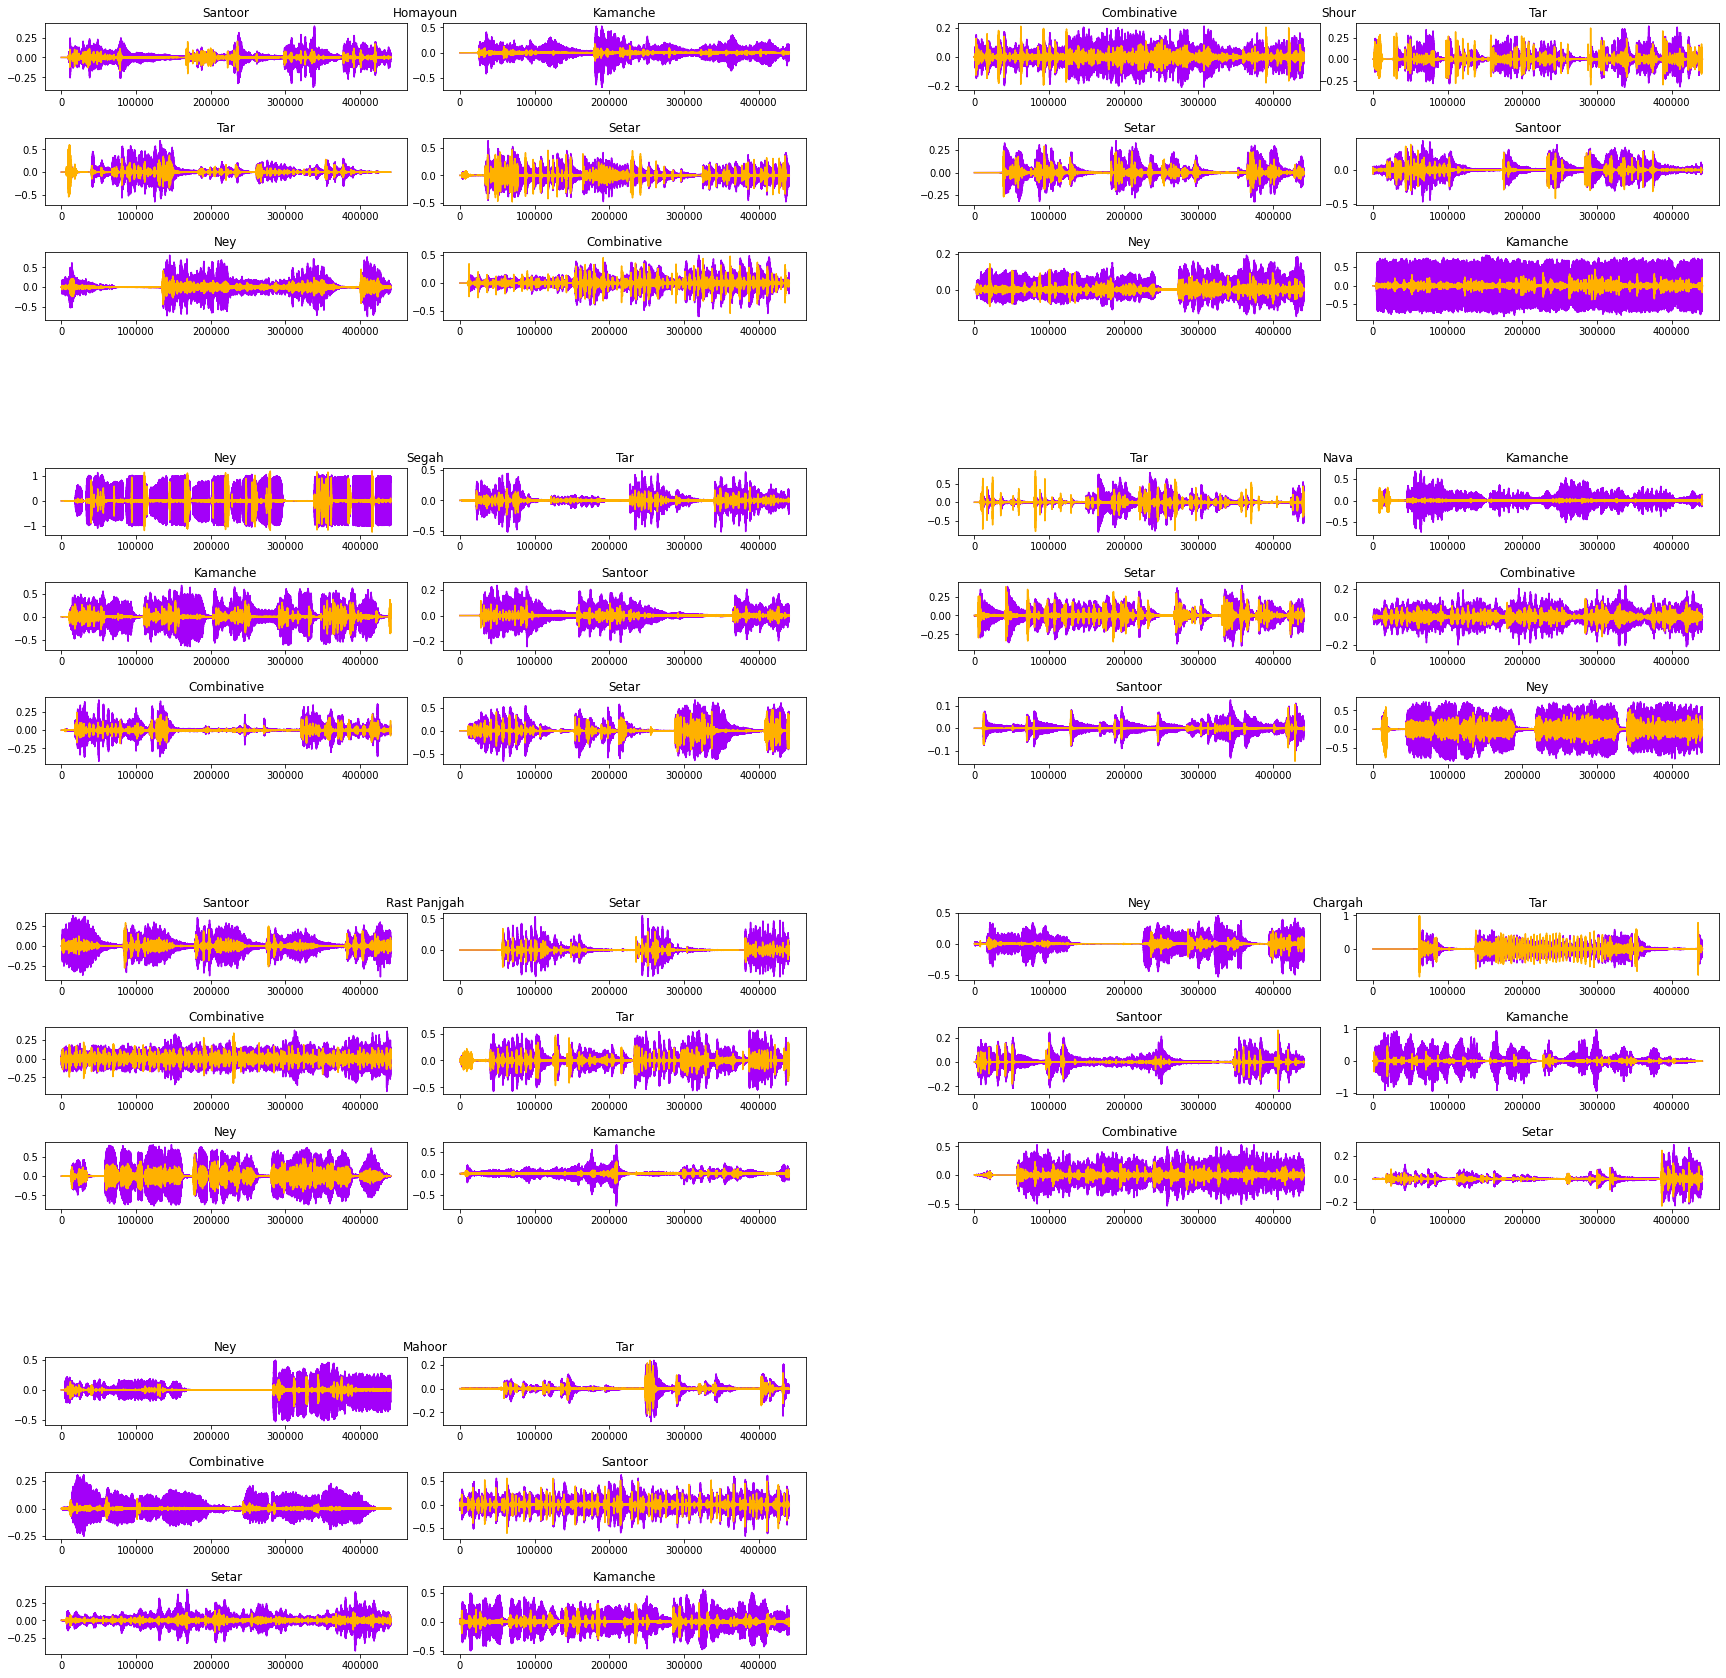
\includegraphics[width=0.5\linewidth]{Photo/27}
	\caption[شمایی از \lr{Harmonics and Perceptrual}]{شمایی از \lr{Harmonics and Perceptrual}}
	\label{fig:27}
\end{figure}


\lr{Tempo BMP (beats per minute)} :\newline
تعداد ضربات در یک دقیقه را نشان می دهد. به عنوان مثال، سرعتی که با 60 BPM مشخص شده است به این معنی است که یک ضرب دقیقاً یک بار در ثانیه به صدا در می آید. سرعت 120 ضربان در دقیقه دو بار سریعتر است، با دو ضربه در ثانیه.
\begin{figure}[h]
	\centering
	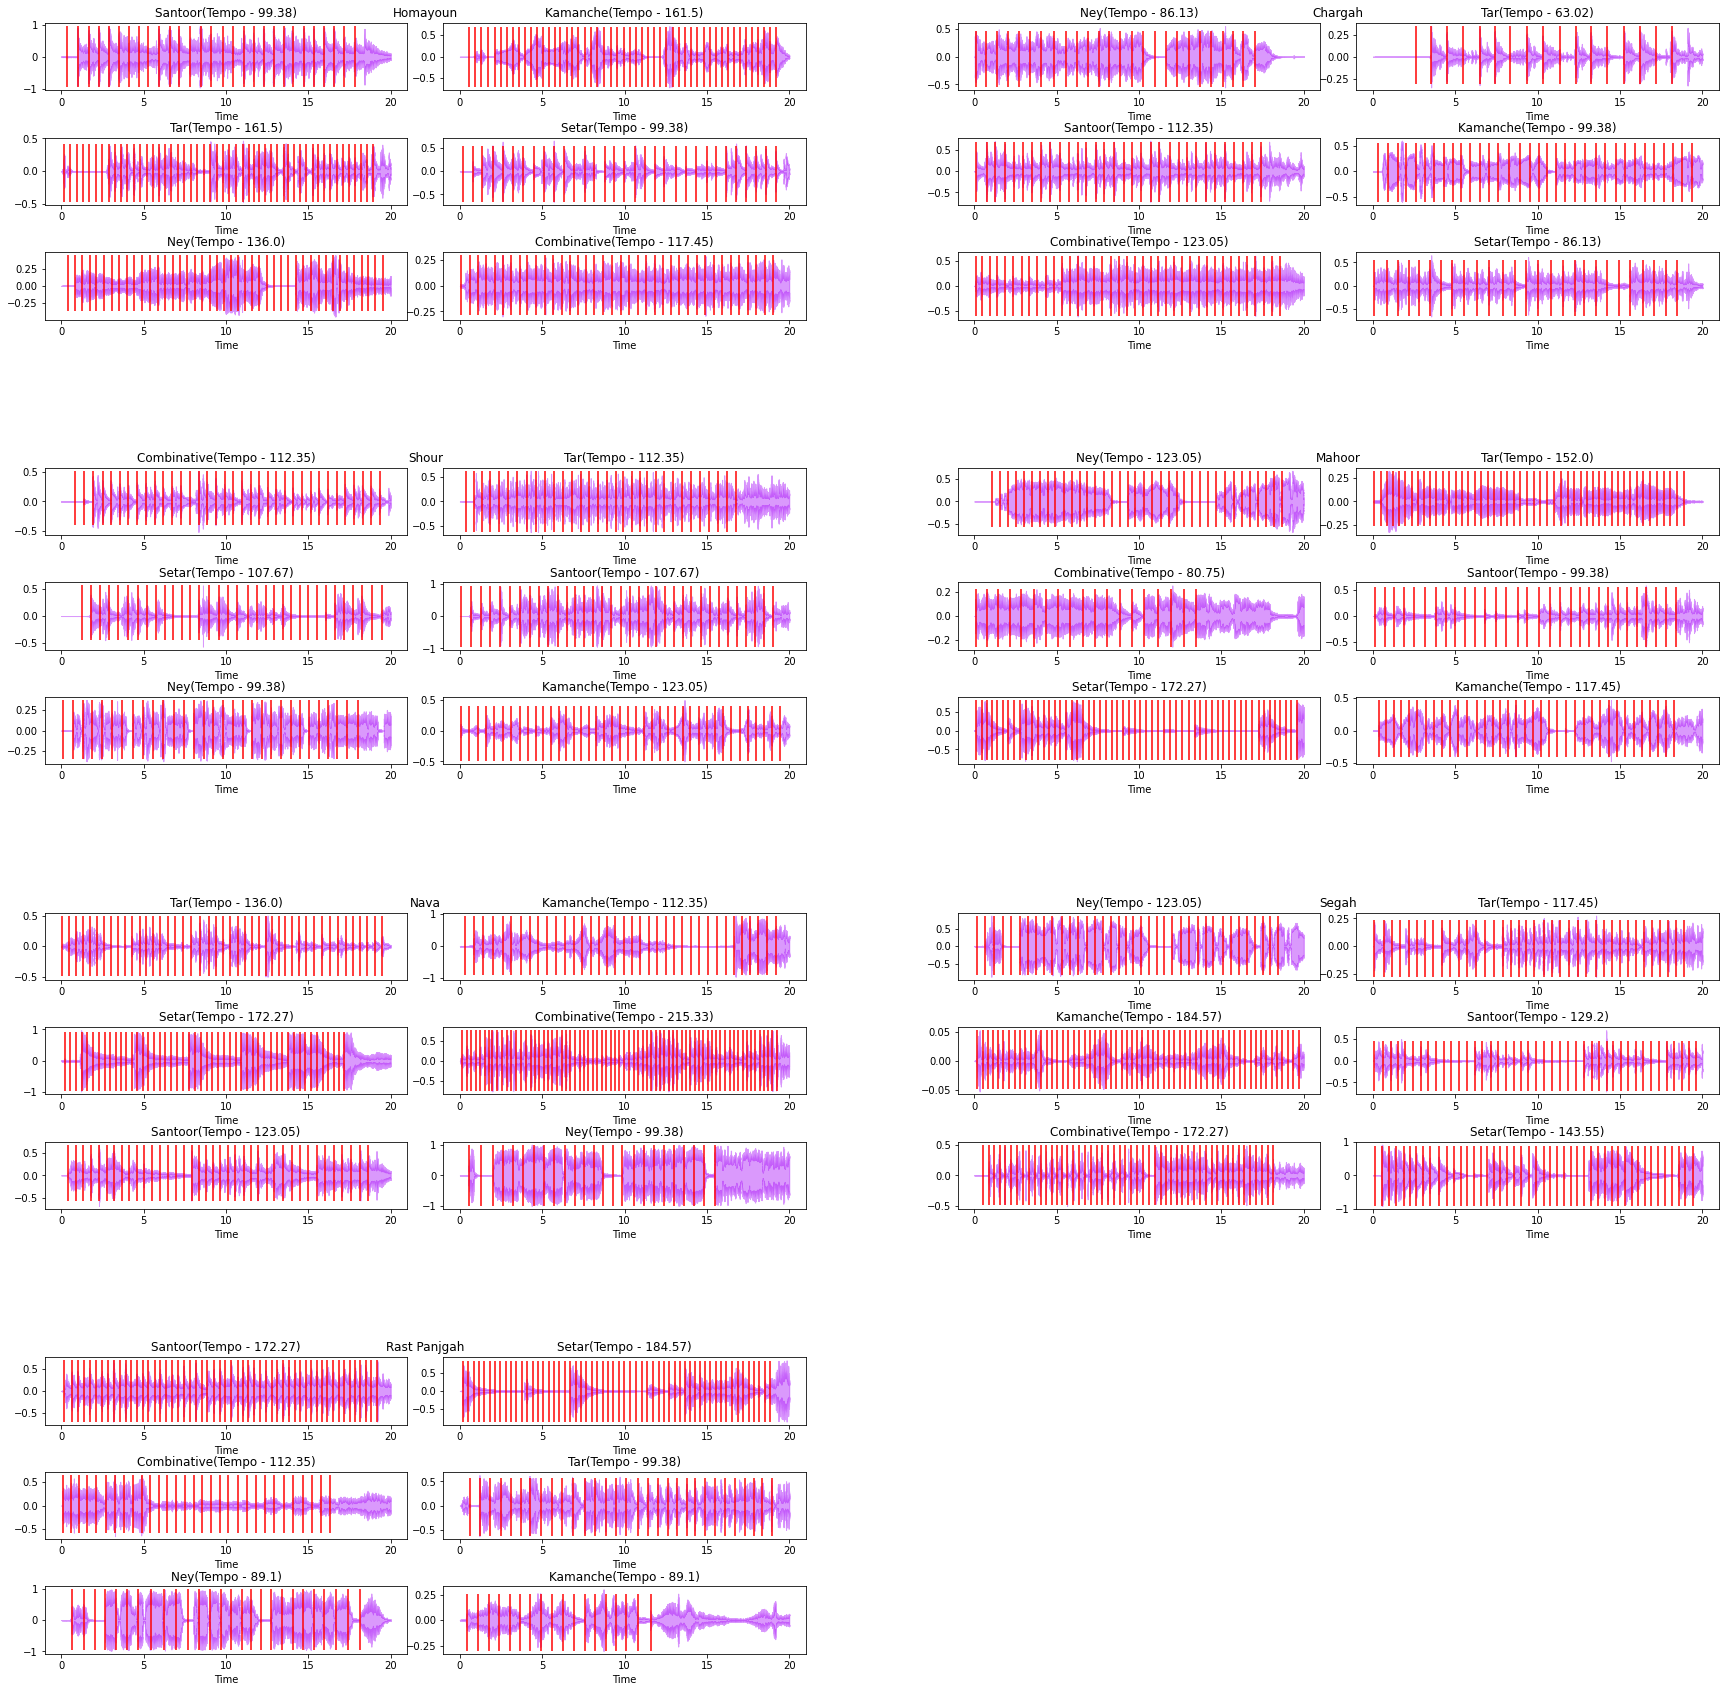
\includegraphics[width=0.5\linewidth]{Photo/28}
	\caption[نمونه از نمایش تعداد ضربات در دقیقه]{نمونه از نمایش تعداد ضربات در دقیقه}
	\label{fig:28}
\end{figure}



\lr{Mel-Frequency Cepstral Coefficients} : \newline
ضرایب مغزی فرکانس mel (MFCCs) یک سیگنال مجموعه کوچکی از ویژگی ها (معمولاً حدود 10-20) هستند که به طور خلاصه شکل کلی یک پوشش طیفی را توصیف می کنند. در MIR، اغلب برای توصیف تایم استفاده می شود.
\begin{figure}[h]
	\centering
	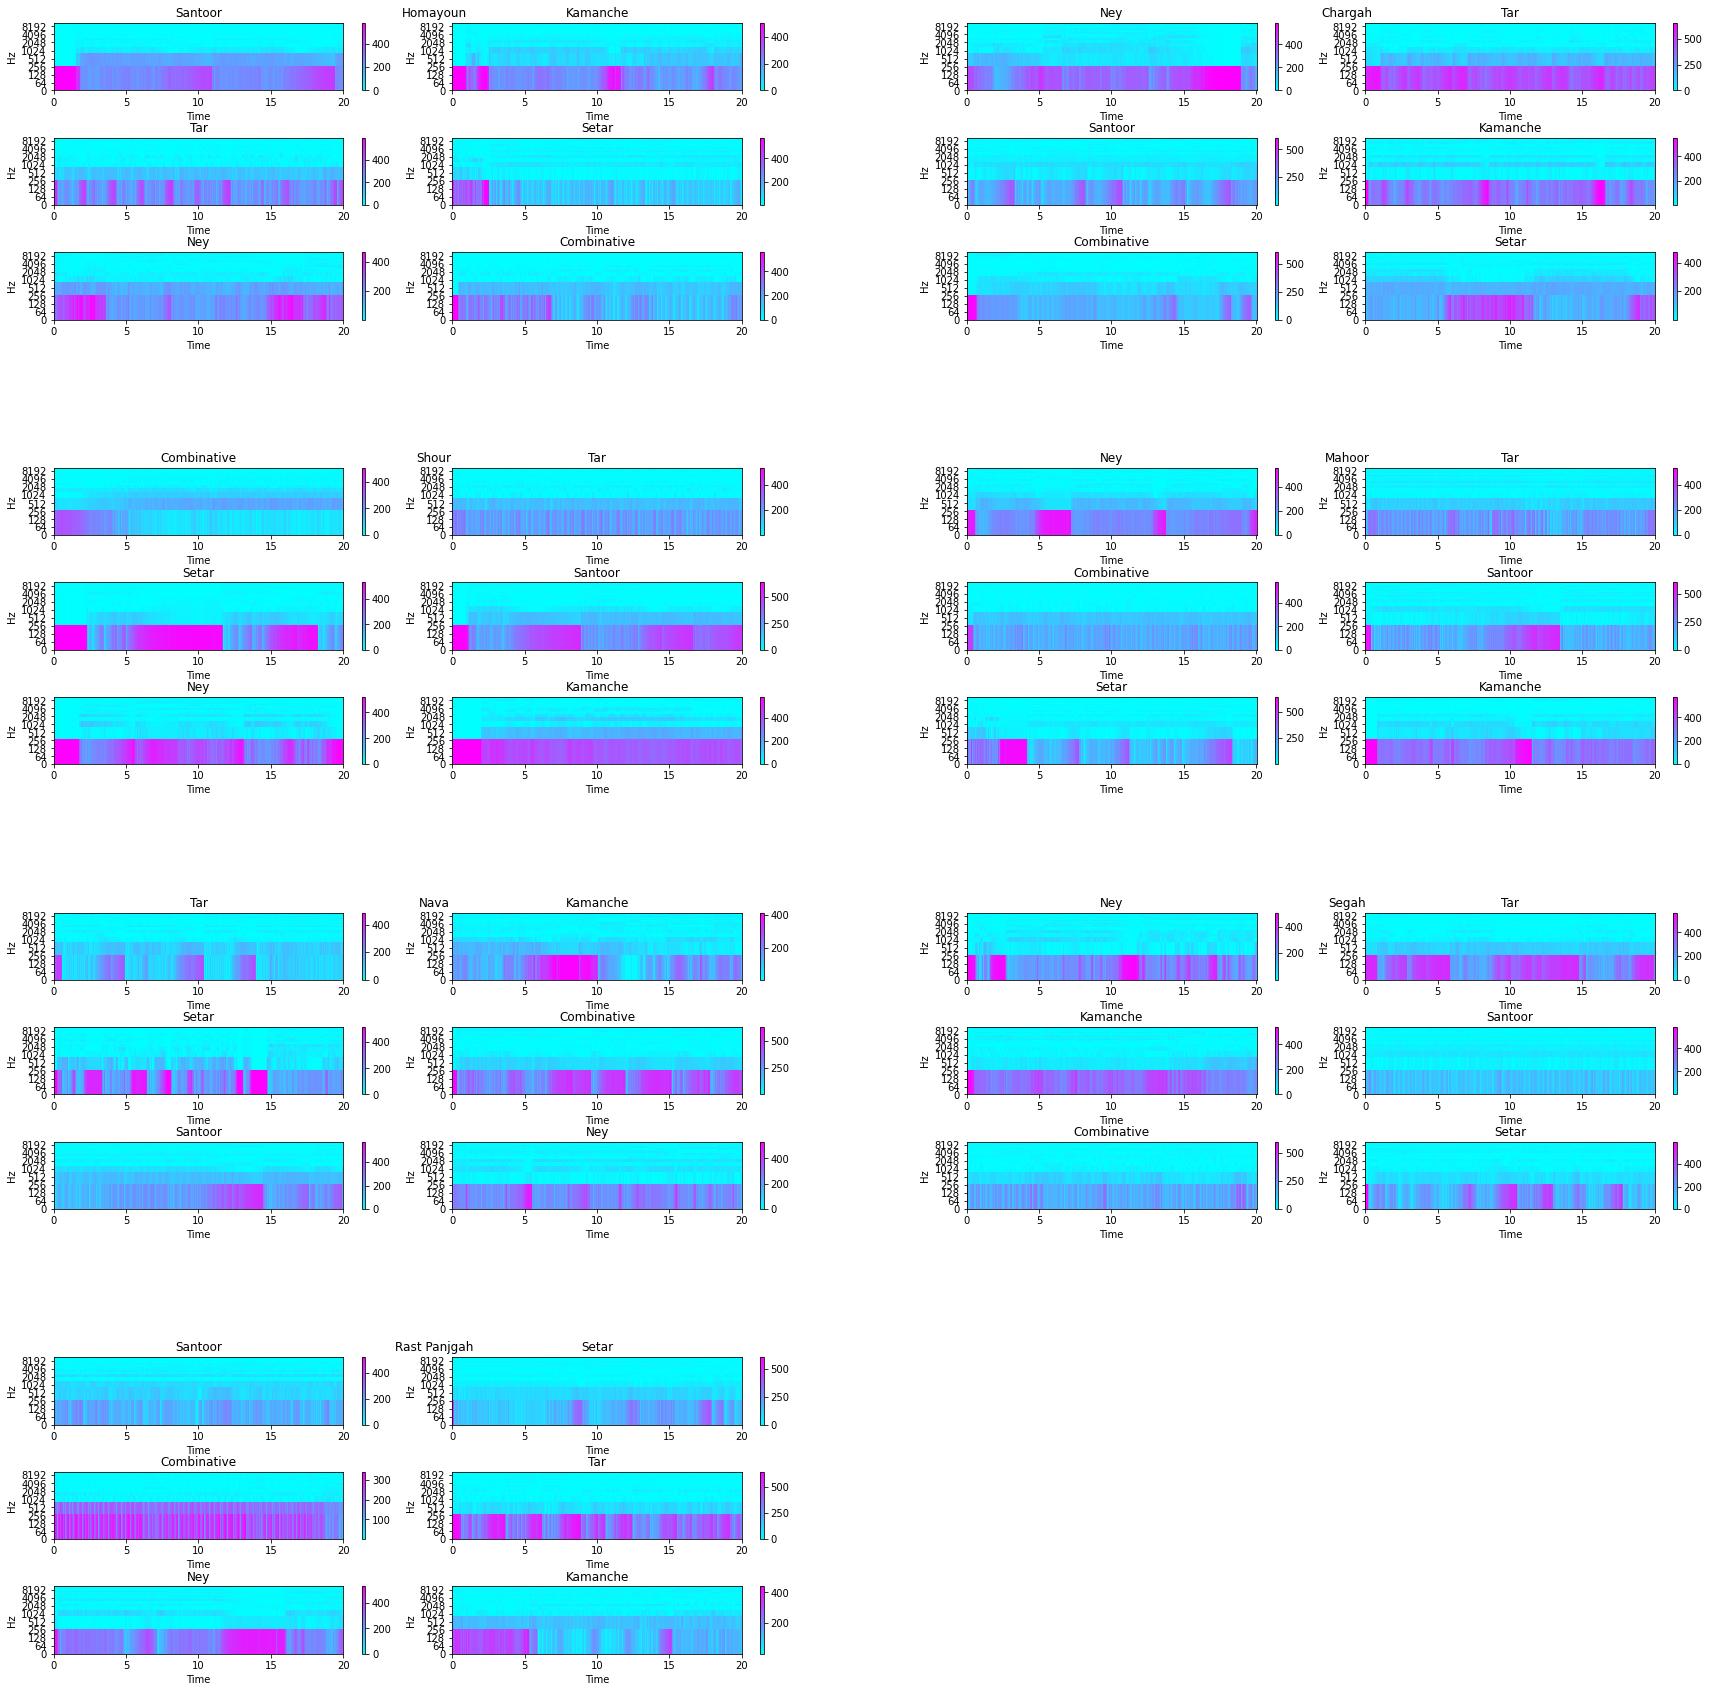
\includegraphics[width=0.5\linewidth]{Photo/32}
	\caption[نمایی از \lr{Mel-Frequency Cepstral}]{نمایی از \lr{Mel-Frequency Cepstral}}
	\label{fig:32}
\end{figure}




\lr{Spectogram} : \newline
طیف‌نگار یک نمایش بصری از طیف فرکانس‌های یک سیگنال است که با زمان تغییر می‌کند. هنگامی که طیف‌نگارها بر روی یک سیگنال صوتی اعمال می‌شوند، گاهی اوقات سونوگرافی، چاپ صوتی یا صوت‌گرام نامیده می‌شوند. هنگامی که داده ها در یک نمودار سه بعدی نمایش داده می شوند، ممکن است نمایش آبشار نامیده شوند.
\begin{figure}[h]
	\centering
	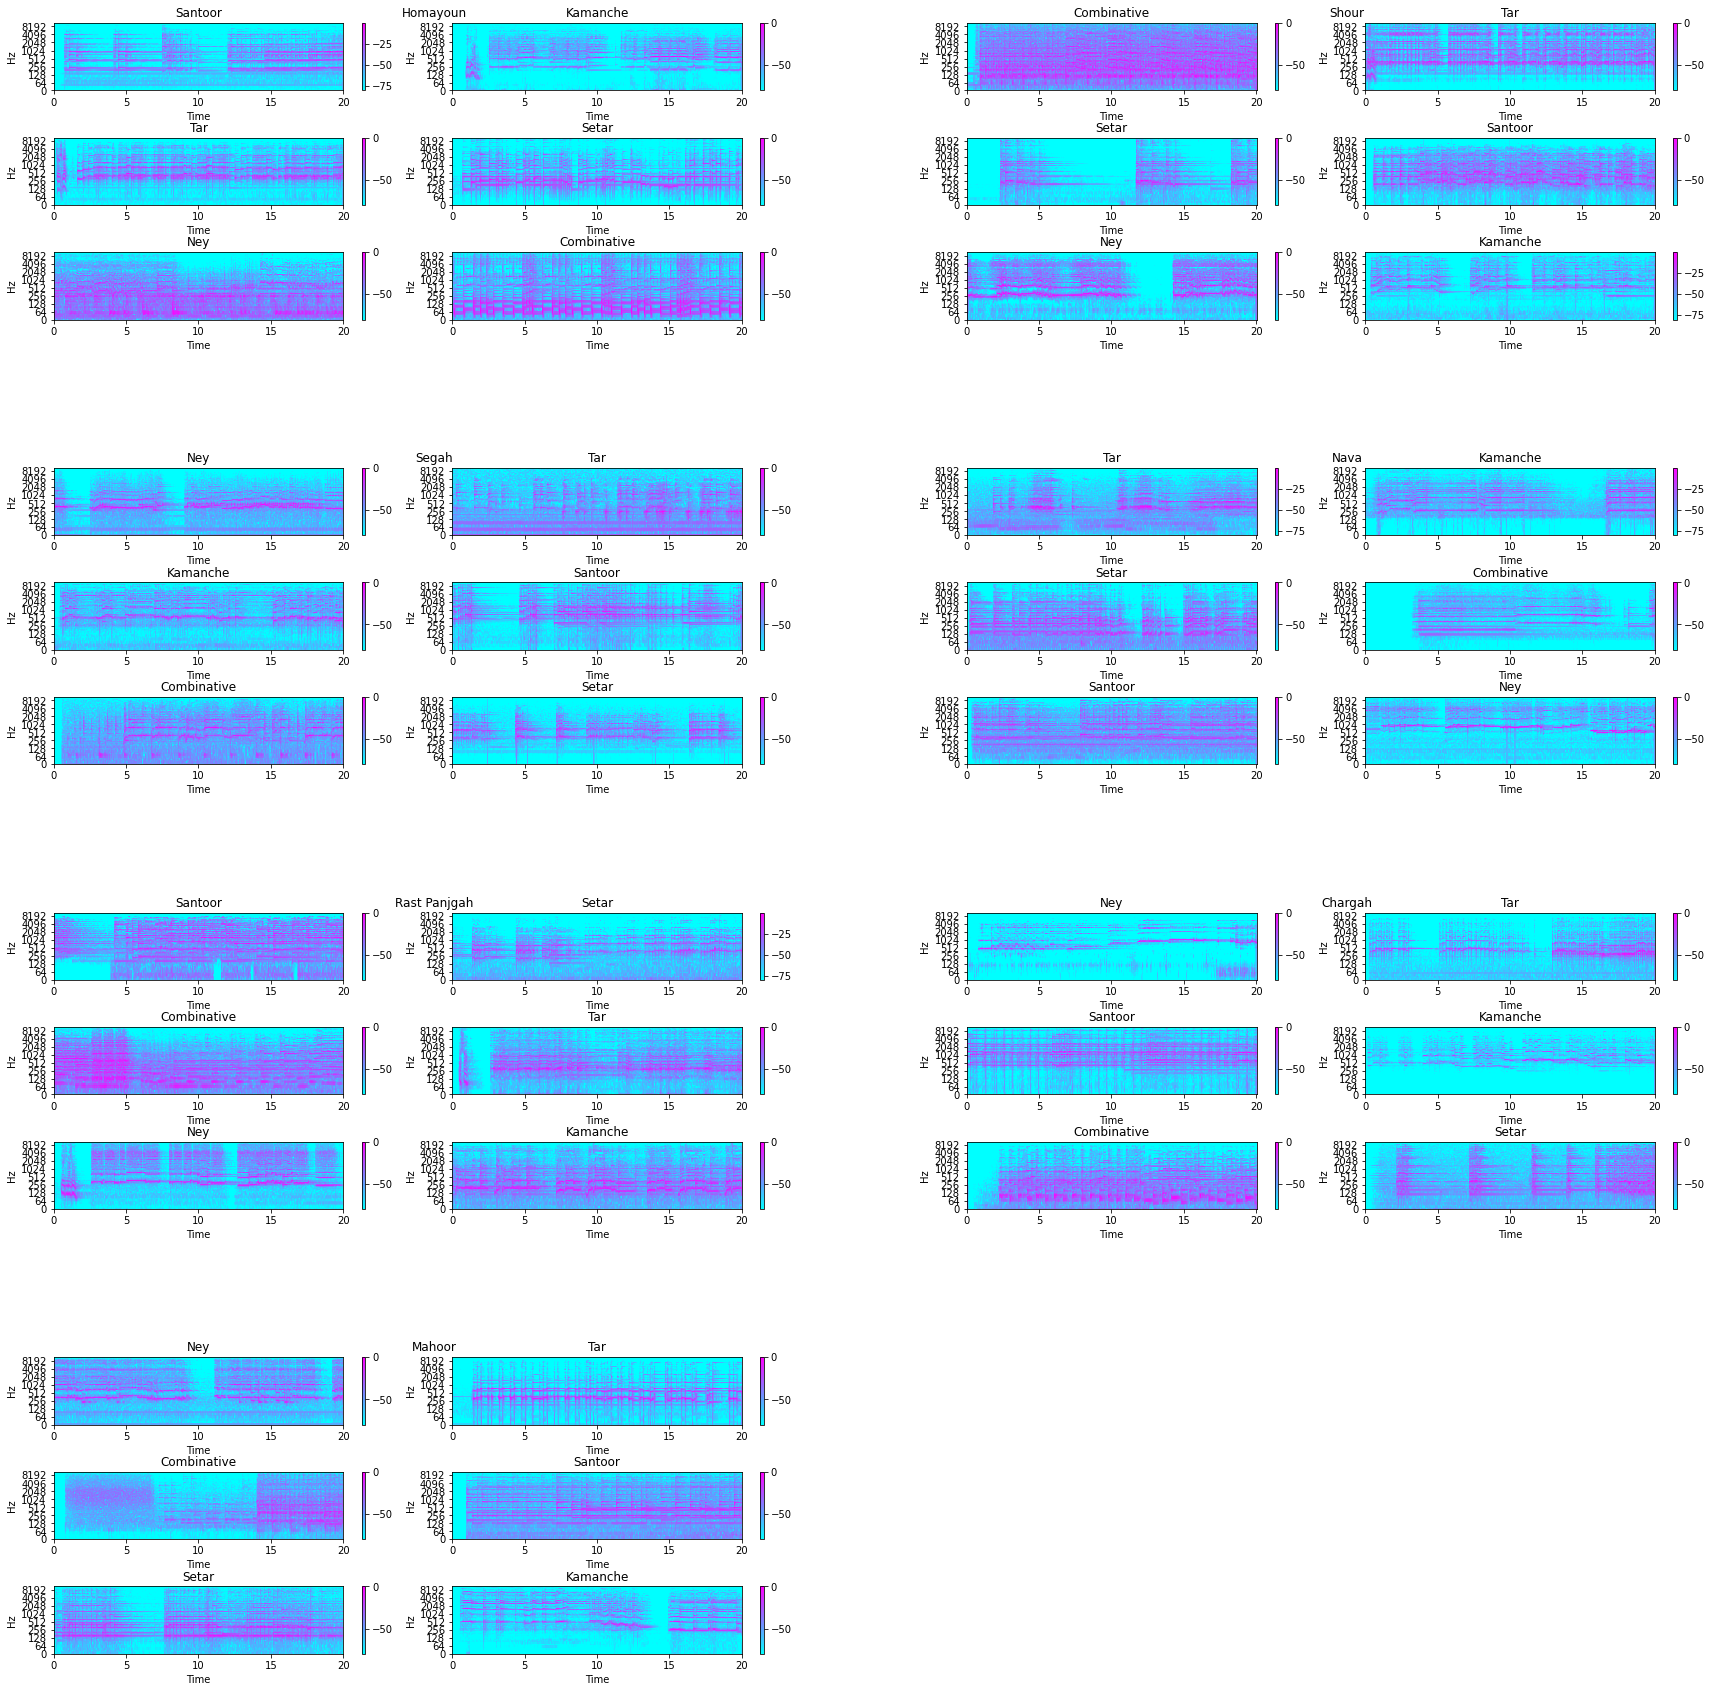
\includegraphics[width=0.5\linewidth]{Photo/34}
	\caption[نمایی از \lr{Spectogram}]{نمایی از \lr{Spectogram}}
	\label{fig:34}
\end{figure}


\lr{Mel Spectogram} : \newline
یک طیف‌نگار mel به صورت لگاریتمی فرکانس‌ها را بالاتر از یک آستانه مشخص (فرکانس گوشه) ارائه می‌کند. به عنوان مثال، در طیف‌نگار با مقیاس خطی، فضای عمودی بین 1000 تا 2000 هرتز نیمی از فضای عمودی بین 2000 هرتز و 4000 هرتز است.
\begin{figure}[h]
	\centering
	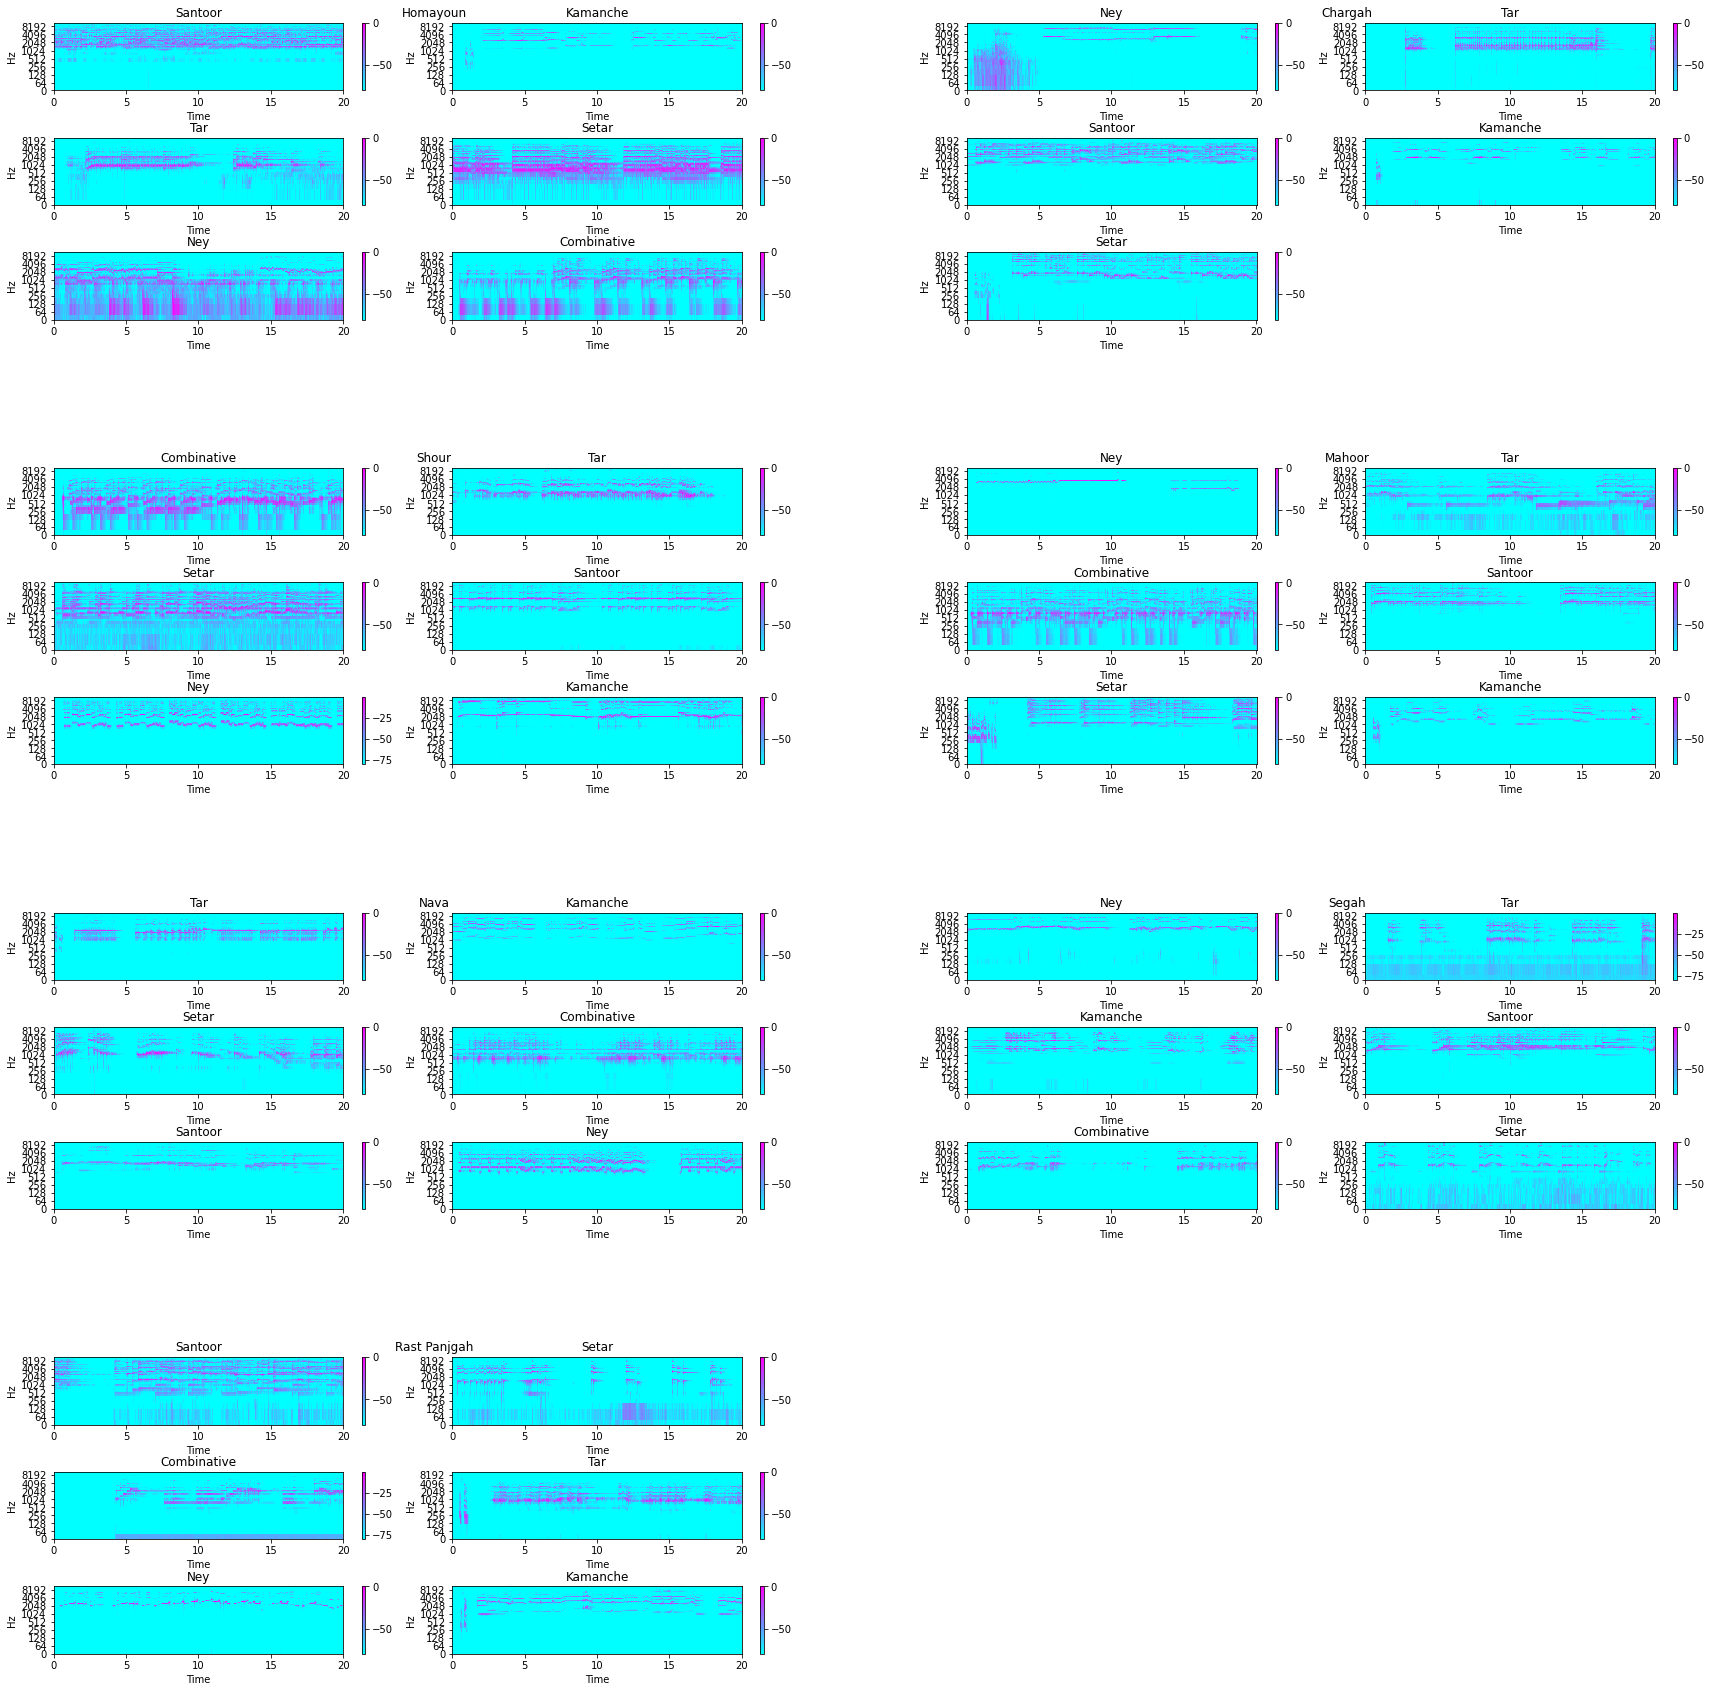
\includegraphics[width=0.5\linewidth]{Photo/33}
	\caption[نمایی از \lr{Mel Spectogram}]{نمایی از \lr{Mel Spectogram}}
	\label{fig:33}
\end{figure}

\newpage
\subsection{۲-۶) ویژگی های طیفی}

برای طبقه بندی، ما از ویژگی های جدید در استفاده خواهیم کرد: گشتاورهای طیفی (مرکز، پهنای باند، چولگی، کشیدگی) و سایر آمارهای طیفی.
\newline
در ادامه \lr{Momens} اصطلاحی است که در فیزیک و آمار استفاده می شود. \lr{Momens} خام و \lr{Momens} محوری وجود دارد.\newline
احتمالاً قبلاً با دو مثال از  \lr{Momens}  آشنا هستید: میانگین و واریانس. اولین  \lr{Momens} خام به عنوان میانگین شناخته می شود. دومین  \lr{Momens} مرکزی به عنوان واریانس شناخته می شود.\newline


مرکز طیفی \lr{Spectral Centroid}: مرکز طیفی نشان می دهد که انرژی یک طیف در کدام فرکانس متمرکز است. این مانند یک میانگین وزنی است:
\begin{figure}[h]
	\centering
	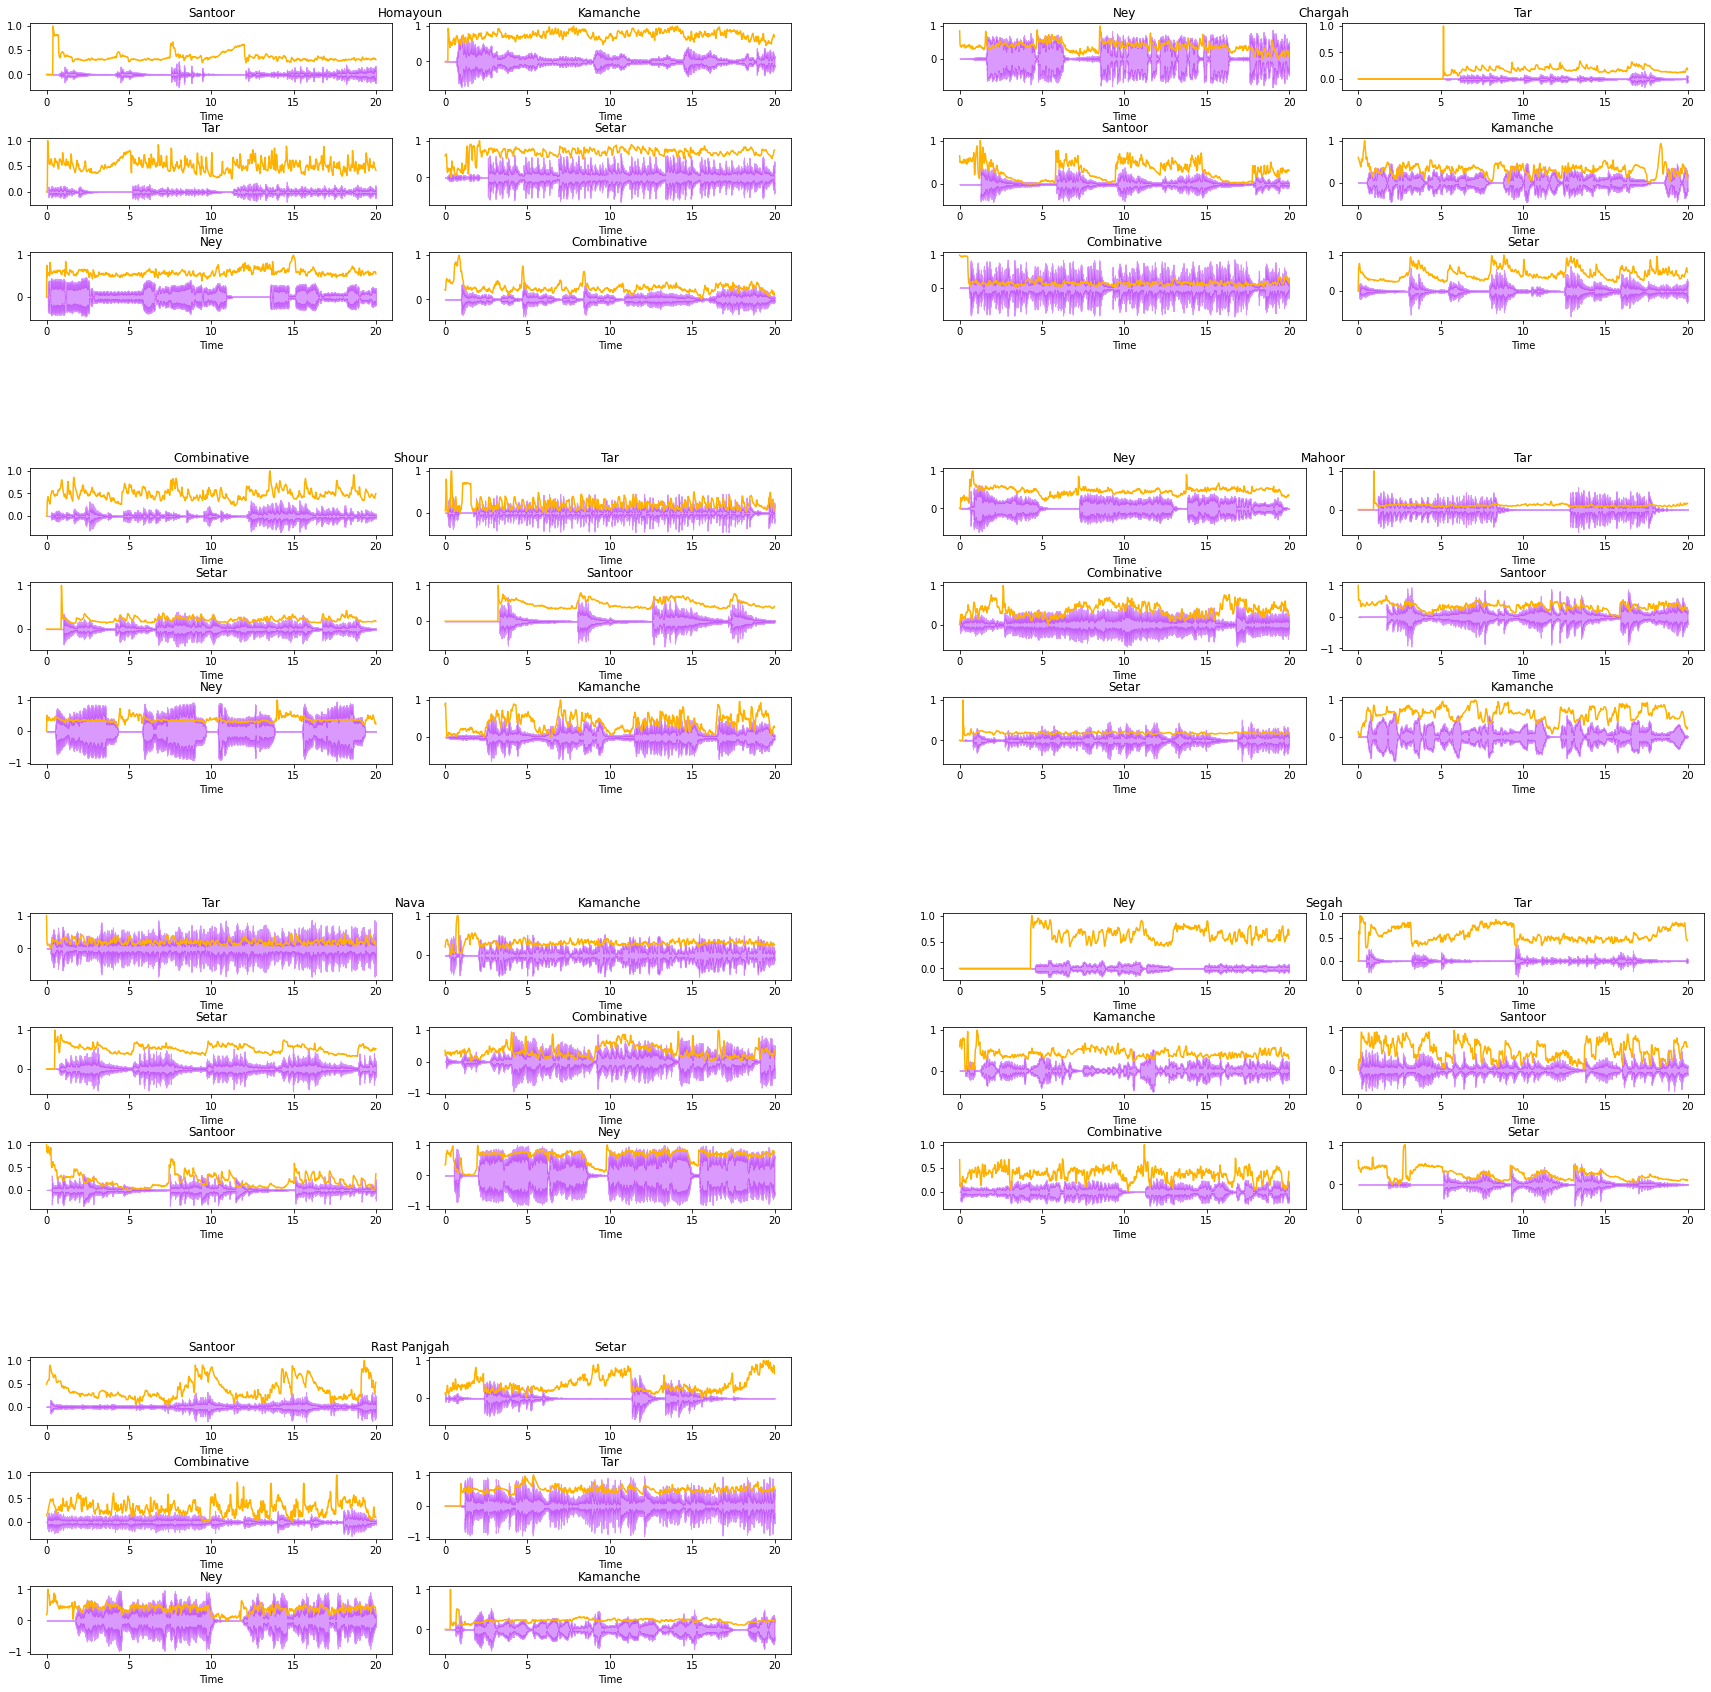
\includegraphics[width=0.5\linewidth]{Photo/29}
	\caption[نمایی از \lr{Spectral Centroid}]{نمایی از \lr{Spectral Centroid}}
	\label{fig:29}
\end{figure}

\begin{equation}
	f_{c}=\dfrac{\sum S(k)\cdot f(k))}{\sum S(k)}
\end{equation}
در معادله بالا S قدر طیفی و f تابع فرکانس است.\newline
پهنای باند طیفی \rl{Spectral Bandwidth} : 
\newline
\begin{figure}
	\centering
	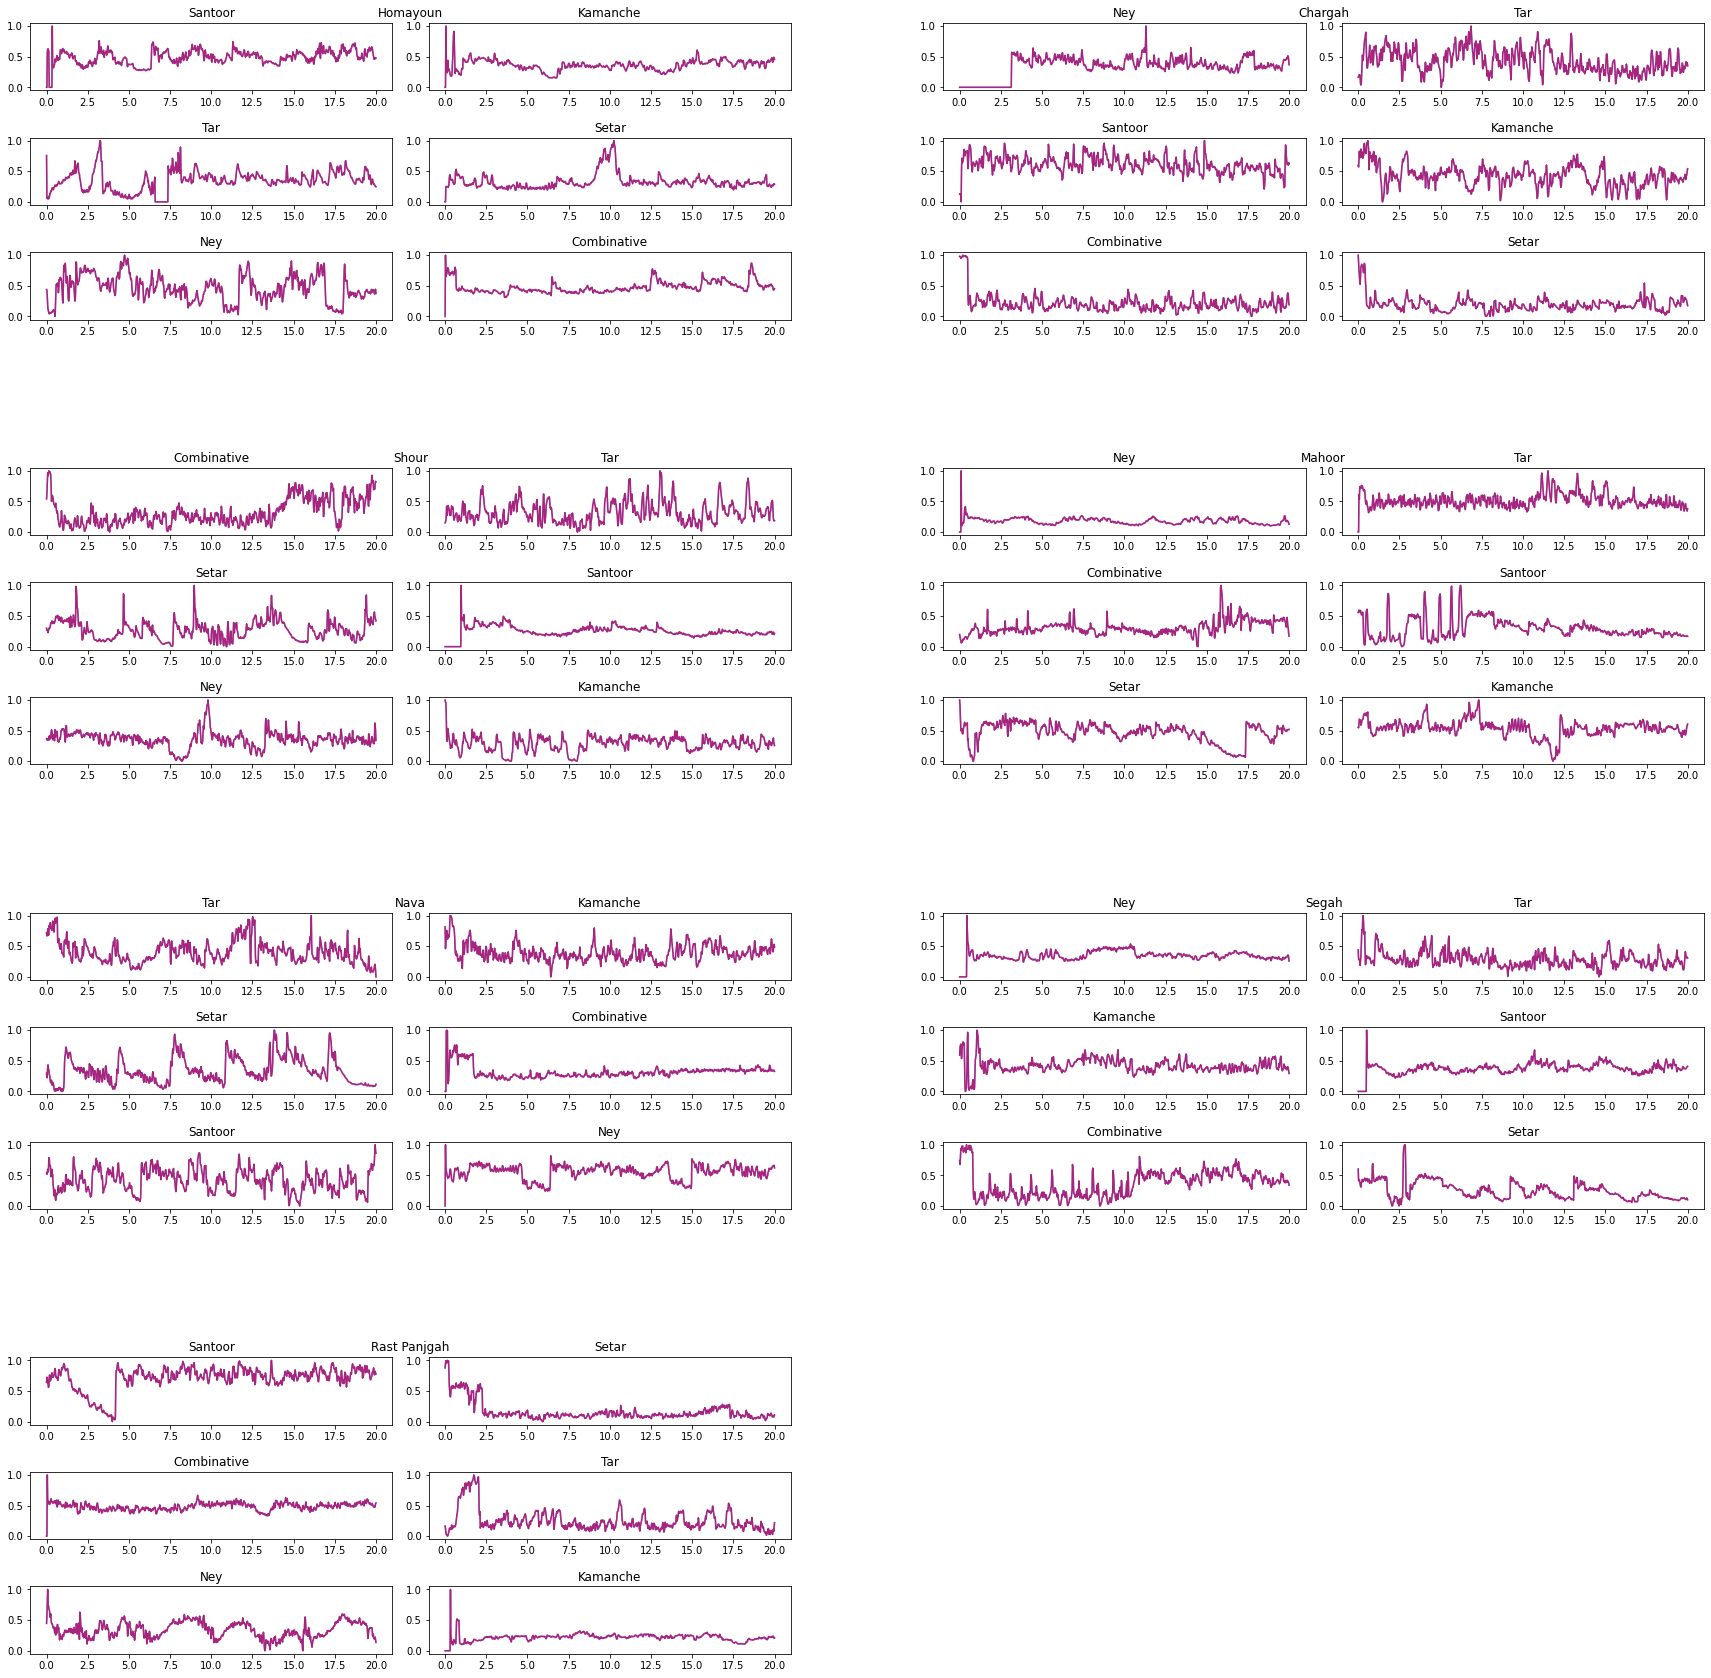
\includegraphics[width=0.5\linewidth]{Photo/31}
	\caption[نمایی از \lr{Spectral Bandwidth}]{نمایی از \lr{Spectral Bandwidth}}
	\label{fig:31}
\end{figure}

پهنای باند طیفی در order دلخواه p به صورت زیر محاسبه می شود:
\begin{equation}
	(\sum S(k)\cdot (f(k)-f_{c})^{p})^{\frac{1}{p}}
\end{equation}
که در معادله بالا S قدر طیفی و f تابع فرکانس است و $f_{c}$ همان مرکز طیفی است.\newline
کنتراست طیفی \lr{Spectral Contrast} :
کنتراست طیفی اوج طیفی، دره طیفی و تفاوت آنها را در هر زیر باند فرکانس در نظر می گیرد.
\begin{figure}[h]
	\centering
	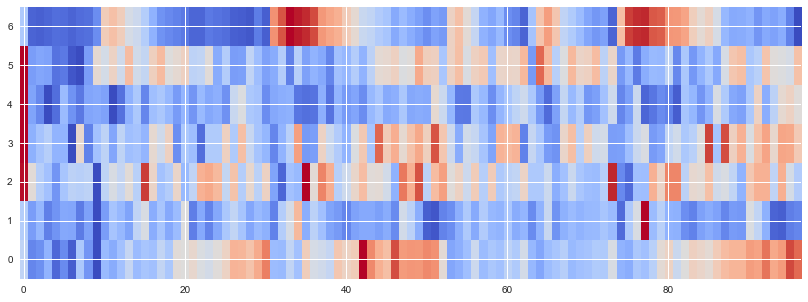
\includegraphics[width=0.7\linewidth]{Photo/8}
	\caption[نمونه ای از کنتراست طیفی]{نمونه ای از کنتراست طیفی}
	\label{fig:8}
\end{figure}
\newpage
طیف رولوف \lr{Spectral Rolloff} :طیفی رولوف فرکانسی را که در زیر آن درصد مشخصی از کل انرژی طیفی قرار دارد را مشخص می کند.\newline

\begin{figure}[h]
	\centering
	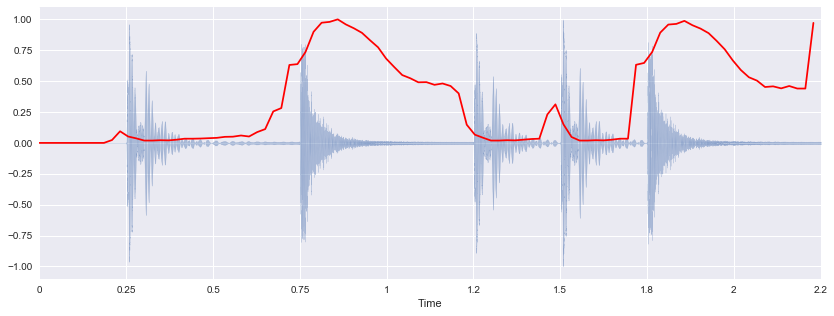
\includegraphics[width=0.7\linewidth]{Photo/9}
	\caption[نمونه ای از طیف رولوف]{نمونه ای از طیف رولوف}
	\label{fig:9}
\end{figure}
همچنین نمونه ی پیاده سازی ما از این طیف به صورت زیر به دست می آيد:
\begin{figure}[h]
	\centering
	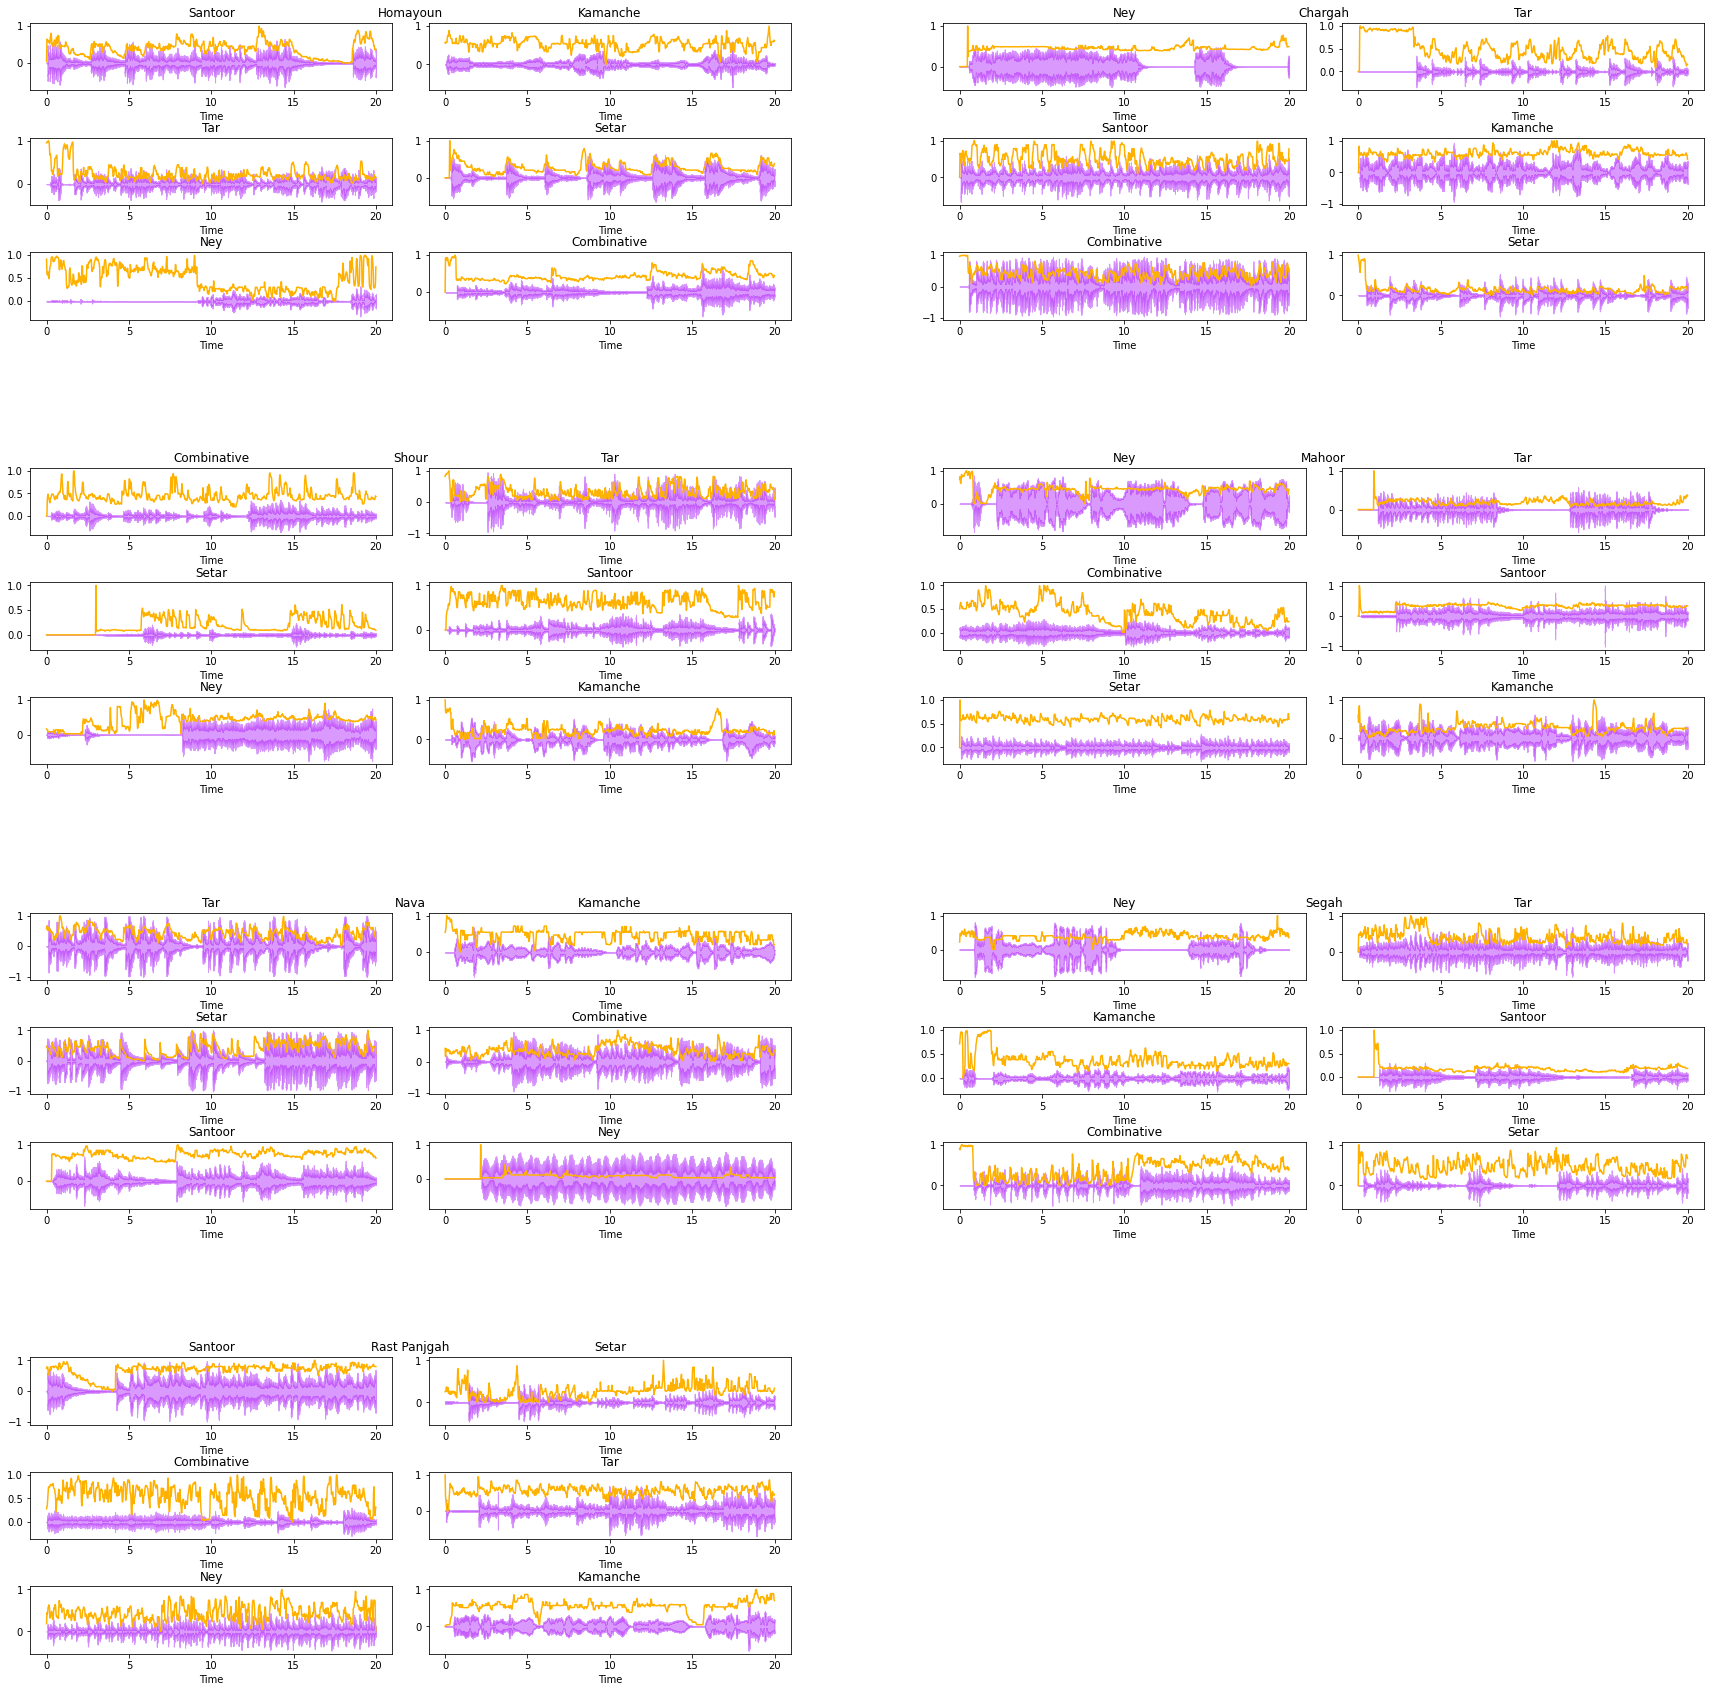
\includegraphics[width=0.7\linewidth]{Photo/30}
	\caption[نمایی از \lr{Spectral Rolloff}]{نمایی از \lr{Spectral Rolloff}}
	\label{fig:30}
\end{figure}

\section{۳) استخراج ویژگی و پیش پردازش داده ها}
بعد از این که توانستیم آشنایی نسبی نسبت به این که یک سیگنال صوتی چیست, چه ویژگی هایی دارد و چگونه می توان به کمک این ویژگی ها آن ها را از هم تشخیص داد و طبقه بندی و خوشه بندی کرد حال باید وارد وادی عملیاتی شده و شروع به پیاده سازی دانش خود بر روی داده ها نماییم.
\subsection{۳-۱) دیتاست}
در این بخش داده های ما شامل ۶۴۸ عدد موسیقی بین ۲۰ ثانیه تا ۱۰ دقیقه است که ترکیبی از دستگاه ها و ساز های مختلف ایرانی است در هم ادقام شده اند و همچنین نوع ساز استفاده شده و دستگاه به کار رفته در موسیقی که درون  دیتاست ما نهادینه شده است به صورت جدول زیر است.\newline
\begin{figure}[h]
	\centering
	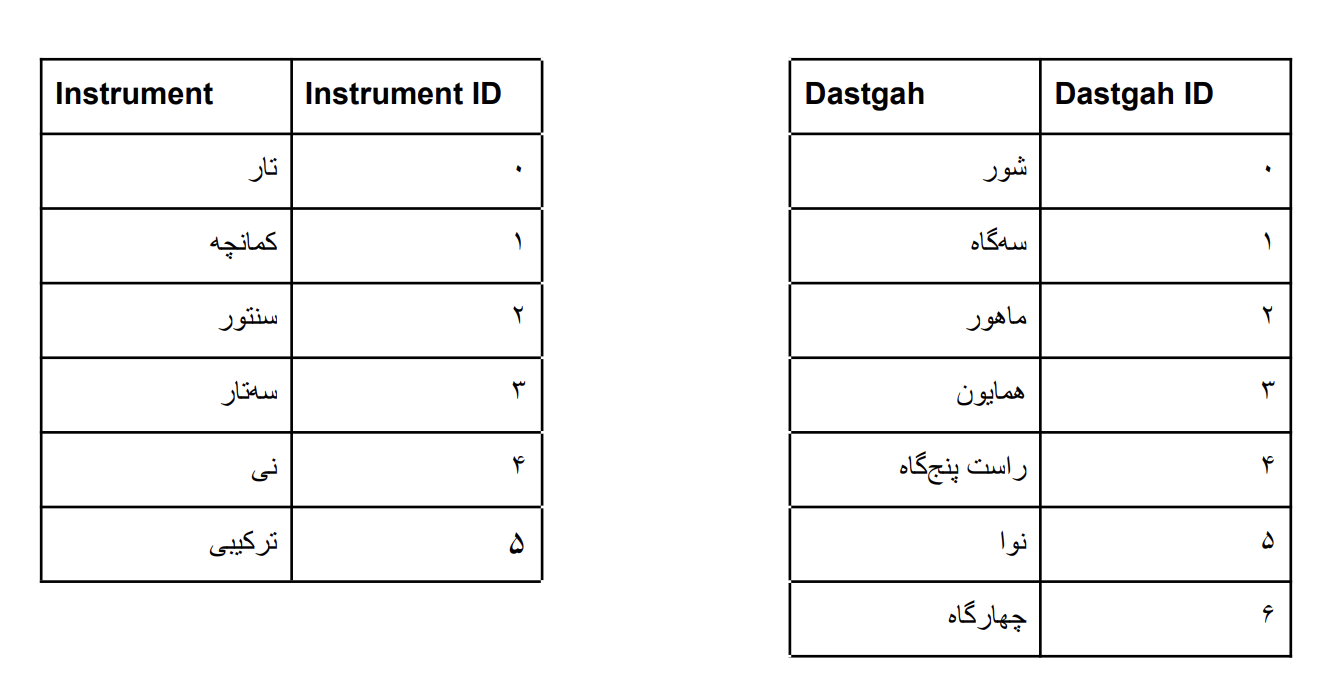
\includegraphics[width=0.7\linewidth]{Photo/10}
	\caption[ویژگی های دیتاست]{ویژگی های دیتاست}
	\label{fig:10}
\end{figure}\newline
همان طور که در شکل بالا مشاهده می شود دستگاه ها و ابزار های موسیقی نام برده شده شاکله کلی دیتاست مار تشکیل می دهند.\newline
در رابطه با این موضوع که هر دستگاه و هر ابزار موسیقی چه ویژگی هایی دارد و چگونه کار می کند به صورت کامل در گزارش اولیه لحاظ شده است و برای جلوگیری از زیاده گویی از تکرار آن صرف نظر می کنیم.\newline
\subsection{۳-۲) استخراج ویژگی}
در ادامه باتوجه به تمامی ویژگی های طیفی که در مورد سیگنال موسیقی بیان کردیم باید برای دیتاست خود که پیش تر اشاره کردیم شامل ۶۴۸ قطعه موسیقی که هر کدام بین ۲۰ ثانیه الی ۱۰ دقیقه هستند, به استخراج ویژگی از این دیتاست برسیم.\newline
به طورکلی در پایتون از دو روش کلی برای استخراج ویژگی ها استفاده می کنیم که مفاهیم بخش دوم را به تصویر می کشند:
۱)\lr{librosa}:یک بسته پایتون برای تجزیه و تحلیل موسیقی و صدا است. بلوک های ساختمانی لازم برای ایجاد سیستم های بازیابی اطلاعات موسیقی را فراهم می کند.\newline
۲)\lr{text}:یک کتابخانه پایتون برای استخراج ویژگی های است. این روش با هدف پرداختن به نقاط ضعف کتابخانه های موجود و تسهیل استفاده مشترک با چارچوب های مدرن یادگیری ماشین نوشته شده است.
\newline
حال بعد از بررسی کامل مراحلی که در بخش ۲ دیدم ویژگی ها مختلفی را از سیستم خود استخراج می کنیم که در ادامه مطلب با بررسی این ویژگی ها می توان از آنها در طبقه بندی و خوشه بندی دیتاست خود استفاده کنیم که در این رابطع در ادامه به تفصیل صحبت خواهیم کرد.\newline
ویژگی ها استخراج شده به شرح زیر خواهند بود:\newline
\begin{latin}
1) chroma-stft-mean-1 $\;\;\;\;\;\;\;\;\;\;$ 2) chroma-stft-mean-3  $\;\;\;\;\;\;\;\;\;\;$ 3) chroma-stft-mean-5  \newline 4) chroma-stft-mean-7 $\;\;\;\;\;\;\;\;\;\;$
5) chroma-stft-mean-9 $\;\;\;\;\;\;\;\;\;\;$ 6) chroma-stft-mean-11 $\;\;\;\;\;\;\;\;\;\;$ \newline         7) chroma-stft-std-1 $\;\;\;\;\;\;\;\;\;\;\;\;\;\;$ 8) chroma-stft-std-3 $\;\;\;\;\;\;\;\;\;\;\;\;\;$ 9) chroma-stft-std-5 \newline
10) chroma-stft-std-7 $\;\;\;\;\;\;\;\;\;\;\;\;$ 11) chroma-stft-std-9 $\;\;\;\;\;\;\;\;\;\;\;$ 12)  chroma-stft-std-11 \newline
13) rms-mean $\;\;\;\;\;\;\;\;\;\;\;\;\;\;\;\;\;\;\;\;\;\;$   14) num-zerocrossing $\;\;\;\;\;\;\;\;\;\;\;$ 15) mfcc-mean-1 \newline
16) mfcc-mean-3 $\;\;\;\;\;\;\;\;\;\;\;\;\;\;\;\;\;$ 17) mfcc-mean-5 $\;\;\;\;\;\;\;\;\;\;\;\;\;\;\;\;\;\;$ 18) mfcc-mean-7 \newline
19) mfcc-mean-11 $\;\;\;\;\;\;\;\;\;\;\;\;\;\;\;\;\;$ 20) mfcc-mean-13 $\;\;\;\;\;\;\;\;\;\;\;\;\;\;\;\;\;$ 21) mfcc-std-2 \newline
22) mfcc-std-4 $\;\;\;\;\;\;\;\;\;\;\;\;\;\;\;\;\;\;\;\;\;\;$ 23) mfcc-std-6 $\;\;\;\;\;\;\;\;\;\;\;\;\;\;\;\;\;\;\;\;\;\;\;$ 24) mfcc-std-8 \newline
25) mfcc-mean-10 $\;\;\;\;\;\;\;\;\;\;\;\;\;\;\;\;\;$ 26) mfcc-mean-12 $\;\;\;\;\;\;\;\;\;\;\;\;\;\;\;\;\;$ 27) mfcc-skewness-1 \newline
28) mfcc-skewness-3 $\;\;\;\;\;\;\;\;\;\;\;\;\;$ 29) mfcc-skewness-5 $\;\;\;\;\;\;\;\;\;\;\;\;\;$ 30) mfcc-skewness-7 \newline
31) mfcc-skewness-9 $\;\;\;\;\;\;\;\;\;\;\;\;\;$ 32) mfcc-skewness-11 $\;\;\;\;\;\;\;\;\;\;\;$ 33) mfcc-skewness-13 \newline
34) mfcc-kurtosis-2 $\;\;\;\;\;\;\;\;\;\;\;\;\;\;\;$ 35) mfcc-kurtosis-4 $\;\;\;\;\;\;\;\;\;\;\;\;\;\;\;$ 36) mfcc-kurtosis-6 \newline
37) mfcc-kurtosis-8 $\;\;\;\;\;\;\;\;\;\;\;\;\;\;\;$ 39) mfcc-kurtosis-10 $\;\;\;\;\;\;\;\;\;\;\;\;\;$ 40) mfcc-kurtosis-12 \newline
\end{latin} 
همان طور که در بالا قابل مشاهده است ۴۰ ویژگی از دیتاست خود با تمامی اطلاعاتی که در بخش قبل به آن اشاره کردیم استخراج می کنیم که شکل و چهار چوب آن از نام آن ها مشخص است.\newline
در ادامه باید به این مسیله بپردازیم که تاثیر این ویژگی ها و ارتباط آن ها با دستگاه ها را مورد بررسی قرار می دهیم به نحوی که ببینیم کدام ویژگی می تواند در ادامه خواست های ما را بهتر برآورد کند و کدام ویژگی ها در برآورده کردن خواست ما توان کمتری دارد.\newline
برای فهمیدن این موضوع از \lr{correlation matrix} مربوط به این ویژگی ها استفاده می کنیم.\newline
همان طور هم که می دانیم  \lr{correlation matrix} یا ماتریس همبستگی جدولی است که ضرایب همبستگی را برای متغیرهای مختلف نشان می دهد. ماتریس همبستگی بین تمام جفت مقادیر ممکن در یک جدول را نشان می دهد. این ابزار قدرتمندی برای خلاصه کردن یک مجموعه داده بزرگ و شناسایی و تجسم الگوها در داده های داده شده است.\newline
باتوجه به آن چه که گفته شد ماتریس همبستگی ما به صورت زیر به دست می آید:
\begin{figure}[h]
	\centering
	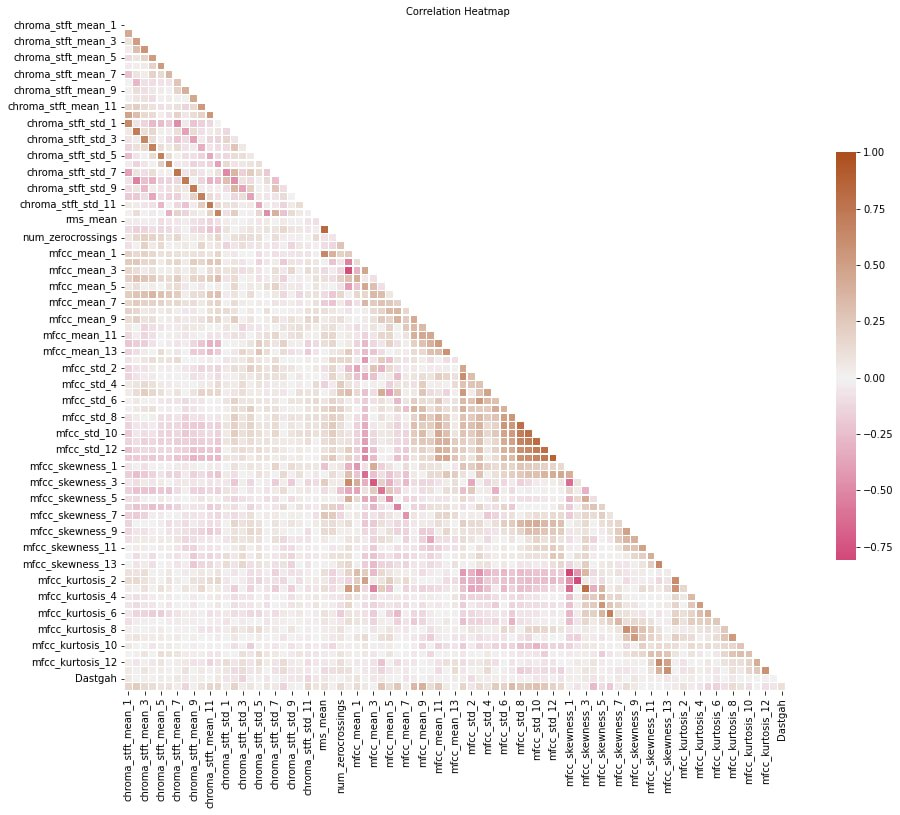
\includegraphics[width=0.5\linewidth]{Photo/11}
	\caption[ماتریس همبستگی]{ماتریس همبستگی}
	\label{fig:11}
\end{figure}
\newpage
همان طورکه از ماتریس همبستگی مشخص است بین ویژگی ها و دستگاه \lr{correlation} زیادی دیده نمی شود پس می توان فهمید برای طبقه بندی داده ها به چیزی بیشتر از یک مدل خطی نیاز داریم که در اداکه بیشتر به آن می پردازیم.
در ادامه نکته مهم دیگری که باید به آن بپردازیم نحوه توزیع داده است زیرا اگر نحوه توزیع داده ها خیلی از هم متفاوت باشد باید از طریق وزن دهی عملیات را پبش ببریم.
باتوجه به این موضوع نحوه توزیع داده ها برای دستگاه ها و ابزار های موسیقی مختلف که پیشتر در رابطه با آن ها صحبت کردیم به صورت زیر به دست می آید:
\begin{figure}[h]
	\centering
	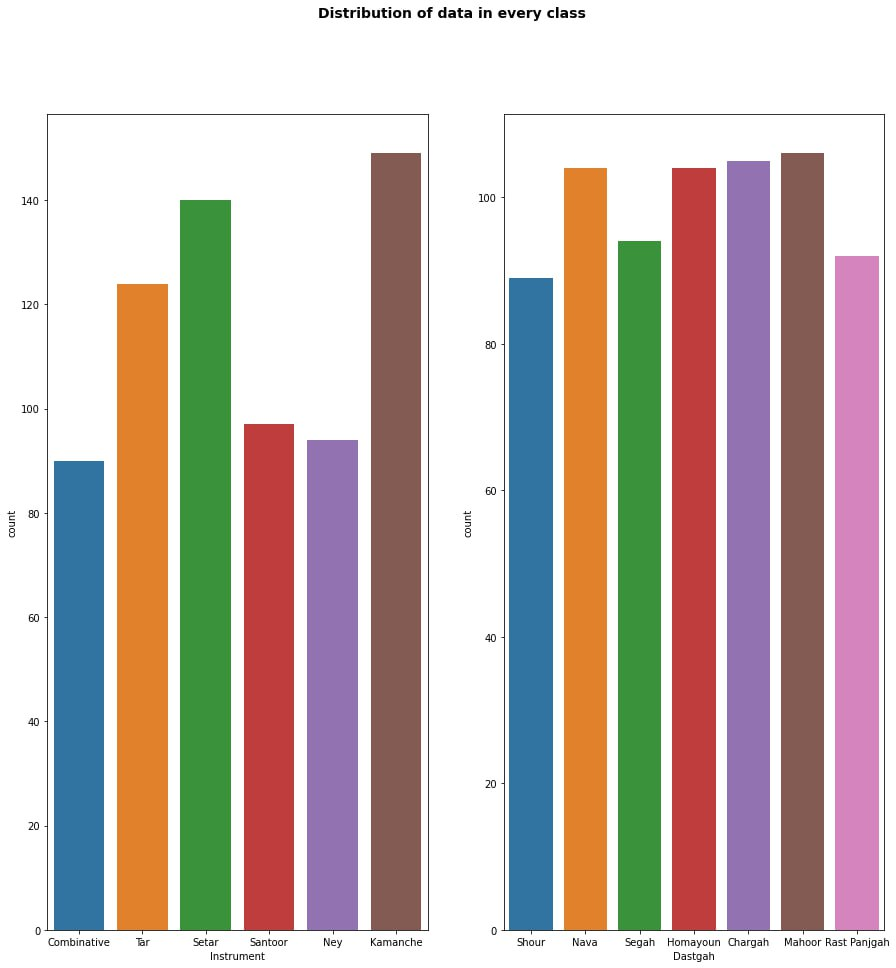
\includegraphics[width=0.41\linewidth]{Photo/12}
	\caption[توزیع داده ها]{توزیع داده ها}
	\label{fig:12}
\end{figure}
\newpage

همان طور که مشخص است از آن جهت که نحوه تقسیم داده ها به نحوی است که خیلی اختلاف ندارند نیاز نیست ضریب خطایی به سیستم بدهیم و از این قسمت به بعد می توان وارد بخش ایجاد مدل برای طبقه بندی داده ها شویم.
\subsection{۳-۳) پیش پردازش داده ها}
در این بخش پیش این که وارد بخش مدل سازی و طبقه بندی داده ها شویم داده های ما نیازمند پردازش اولیه هستند تا بتوان عملیات مدل سازی را بر روی آن ها انجام داد. به عبارت دیگر, پیش پردازش داده فرآیندی است برای تهیه داده های خام و مناسب ساختن آن برای یک مدل یادگیری ماشینی. این اولین و مهم ترین گام در ایجاد یک مدل یادگیری ماشینی است. هنگام ایجاد یک پروژه یادگیری ماشینی، همیشه با داده های تمیز و فرمت شده مواجه نمی شویم.\newline
مراحل پیش پردازش داده ها: حال در ادامه  به مراحل مشخصی بیندازیم که باید طی کنید تا مطمئن شوید داده‌های شما با موفقیت پیش پردازش شده است.\newline
۱)\lr{Data quality assessment}  \newline
۲) \lr{Data cleaning} \newline
۳) \lr{Data transformation} \newline
۴) \lr{Data reduction} \newline


 \lr{Data quality assessment} : داده ‌ها را مورد ببرسی قرار می دهیم و از کیفیت کلی، ارتباط با پروژه خود و سازگاری آن ایده می گیریم. تعدادی از ناهنجاری های داده و مشکلات ذاتی وجود دارد که تقریباً در هر مجموعه داده ای باید به دنبال آنها باشیم..\newline
 
 
 \lr{Data cleaning} : پاکسازی داده ها , فرآیند افزودن داده های از دست رفته و تصحیح، تعمیر یا حذف داده های نادرست یا نامربوط از یک مجموعه داده است. پاکسازی داده ها مهمترین مرحله پیش پردازش است زیرا اطمینان حاصل می کند که داده های ما برای نیازهای پایین آماده است. \newline
 
 
  \lr{Data transformation} :با پاکسازی داده‌ها، ما قبلاً شروع به اصلاح داده‌های خود کرده‌ایم، اما فرآیند تبدیل داده‌ها به قالب(های) مناسبی که برای تجزیه و تحلیل و سایر فرآیندهای پایین دستی نیاز داریم، آغاز می‌کنیم. \newline
  
  
  \lr{Data reduction} : هرچه باداده های بیشتری کار کنیم، حتی پس از تمیز کردن و تبدیل آن ها، تجزیه و تحلیل آن سخت تر خواهد بود. بسته به وظیفه ای که در دست داریم، ممکن است در واقع داده های بیشتری از آنچه نیاز داریم داشته باشیم. به خصوص هنگام کار با تجزیه و تحلیل متن، بسیاری از گفتار منظم انسان اضافی یا بی ربط به نیازهای محقق است. کاهش داده ها نه تنها تجزیه و تحلیل را آسان تر و دقیق تر می کند، بلکه ذخیره سازی داده ها را کاهش می دهد.\newline
 \newpage
 \begin{figure}[h]
 	\centering
 	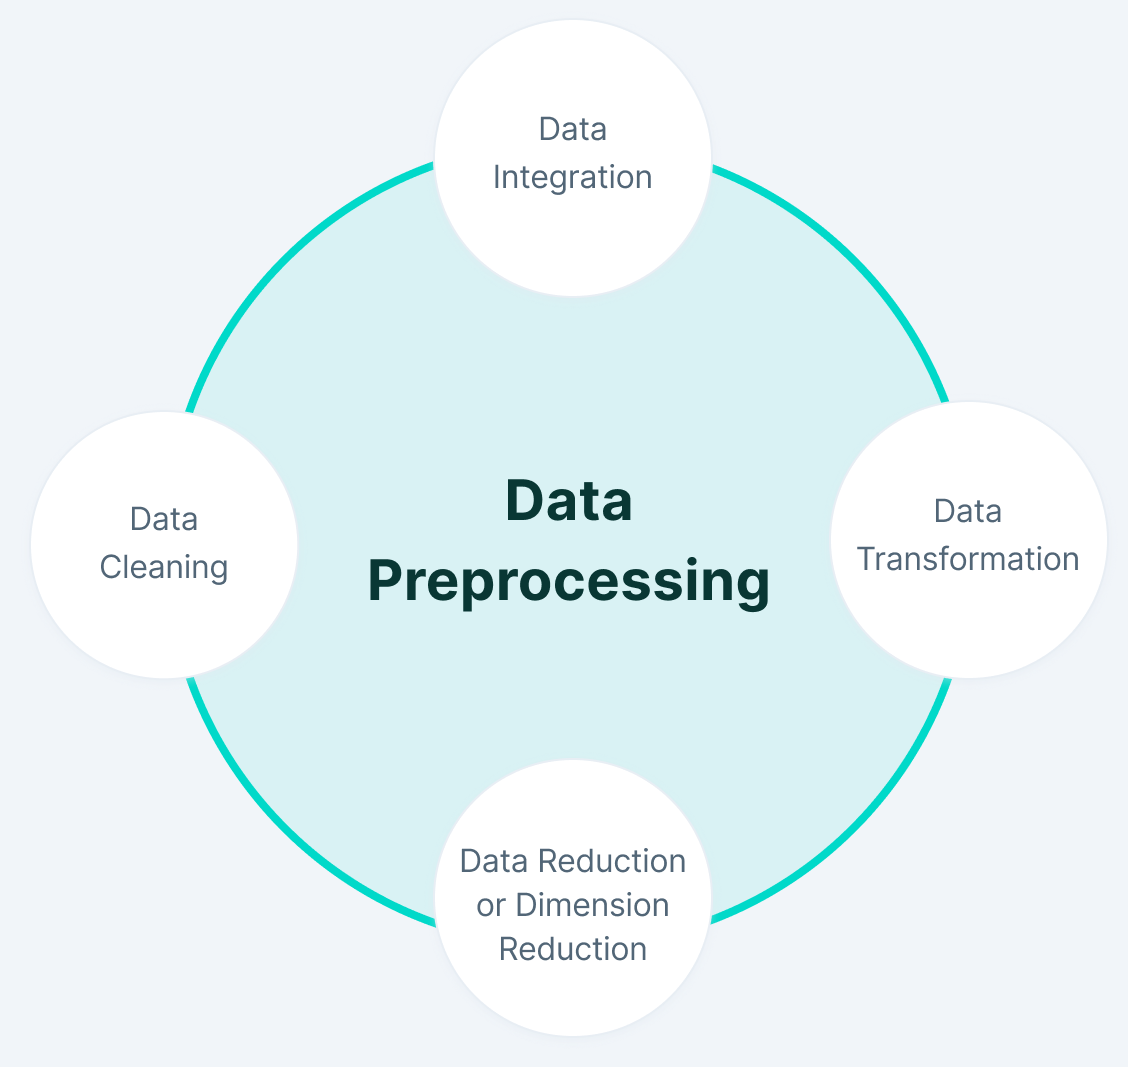
\includegraphics[width=0.5\linewidth]{Photo/13}
 	\caption[پیش پردازش داده]{پیش پردازش داده}
 	\label{fig:13}
 \end{figure}
در این جا ما یک استانداردسازی جایگزین و مقیاس‌بندی ویژگی‌ها برای قرار گرفتن بین حداقل و حداکثر مقدار معین، اغلب بین صفر و یک، قرار می دهیم که به گونه‌ای است که حداکثر مقدار مطلق هر ویژگی به اندازه واحد مقیاس شود.
\newline
انگیزه استفاده از این مقیاس‌بندی شامل استحکام تا انحرافات استاندارد بسیار کوچک ویژگی‌ها و حفظ صفر ورودی در داده‌های پراکنده است.
\subsection{۳-۴) کاهش بعد}
پس از استخراج ویژگی‌ها, از آنجایی که تعداد زیادی ویژگی برای هر صوت داریم، با مشکل پیچیده شدن مدل و سخت شدن طبقه‌بندی مواجه هستیم. برای حل این مشکل روش‌هایی همچون کاهش بعد برای کم کردن تعداد ویژگی‌هایی داریم.
در این پروژه از روش‌های زیر برای کاهش ابعاد داده‌ها استفاده کرده‌ایم:
\begin{itemize}
	\item PCA \newline
 روشی بدون نظارت است که قصد دارد با کمتر کردن تعداد ابعاد داده, کار طبقه‌بندی را ساده تر کند. به عبارت دیگر این روش داده‌ها را به ابعادی دیگر تصویر می‌کند که واریانس آن بعد بیشترین حد باشد.
	با توجه به دو نمودار زیر می‌توان ایده‌ای از تعداد PCAهای مورد نیاز برای مجموعه داده خودم بگیریم.
	 با توجه به این شکل متوجه می‌شویم که ۳۰ عدد از ویژگی‌های انتخاب شده ۹۰ درصد واریانس داده‌ها را در بر می‌گیرند. همچنین با توجه به مقدار ویژه‌های بدست آمده مشخص است که شیب اطلاعات از حدود ۳۰ ویژگی به بعد تقریبا کم شده و در نتیجه ویژگی‌ها ممکن است اطلاعات زیادی برای طبقه‌بند ما فراهم نکنند.
	 \begin{figure}[h]
	 	\centering
	 	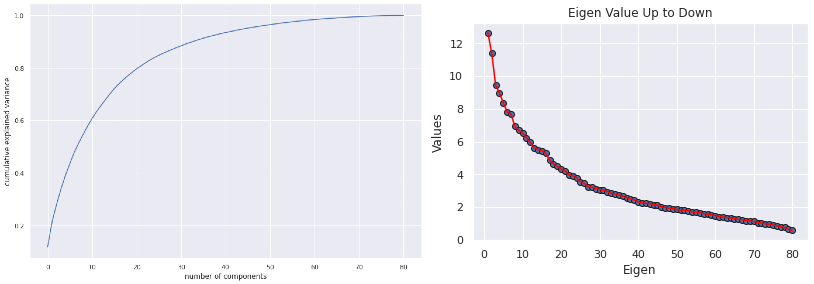
\includegraphics[width=0.7\linewidth]{Photo/36}
	 	\caption[PCA]{PCA}
	 	\label{fig:36}
	 \end{figure}
 
	 
	\item LDA \newline
	این روش با نظارت است که با توجه به کلاس داده‌ها سعی می‌کند ویژگی‌هایی را انتخاب کند که بیشترین جدایی‌پذیری بین کلاسی و بیشترین شباهت درون کلاسی را ایجاد کند. 
	با توجه به نمودار زیر ‌می‌توان ایده‌ای از تعداد LDAهای مورد نیاز برای مجموعه داده خود بگیریم.
	با توجه به این شکل متوجه می‌شویم که حدود ۵ تا از ويژگی‌ها ۹۰ درصد واریانس داده‌ها را در بر می‌گیرند. 
	 \begin{figure}[h]
		\centering
		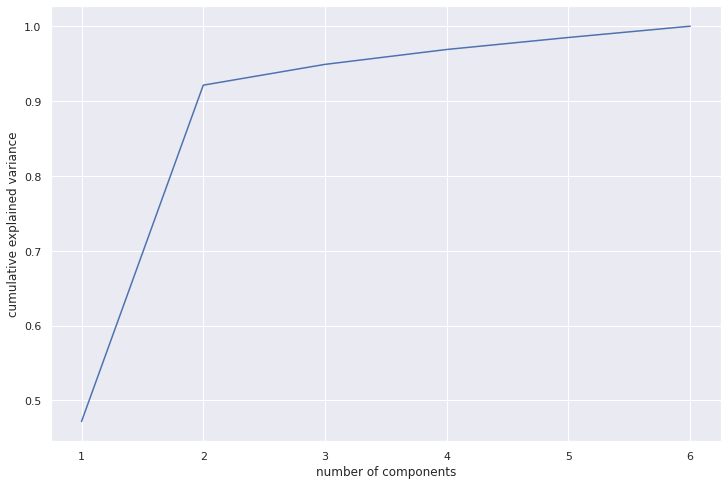
\includegraphics[width=0.7\linewidth]{Photo/LDA}
		\caption[LDA]{LDA}
		\label{fig:lda}
	\end{figure}
	\item \lr{Sequential feature selection} \newline
روش forward selection (SFS) Sequential قصد دارد زیرمجموعه‌ای از ویژگی‌ها پیدا کند. این روش به صورت حریصانه در هر مرحله بهترین ویژگی را انتخاب می‌کند. به عبارتی در هر مرحله با استفاده از تخمین زنی (مدل) تک تک همه ویژگی‌ها را امتحان کرده و ویژگی که بهترین عملکرد را می‌دهد انتخاب می‌کنیم و به زیرمجموعه‌ی خود اضافه می‌کنیم و اینکار را تا جای لازم انجام می‌دهیم. نمودار زیر اثر تعداد ویژگی‌ها و افزایش آن‌ها در خطا و دقت مدل را نشان می‌دهد.\newline
حال در قسمت کدنویسی بعد از پیاده سازی این روش برای کاهش ویژگی ها به ۱۰ عدد نتیجه به دست آمده به صورت زیر خواهد بود:
۱) \lr{chroma-stft-mean-1} $\;\;\;\;\;\;\;\;\;$ ۲) \lr{chroma-stft-mean-2} $\;\;\;\;\;\;\;\;$ ۳) \lr{chroma-stft-mean-5} \newline
۴) \lr{chroma-stft-mean-8} $\;\;\;\;\;\;\;\;\;$ ۵) \lr{chroma-stft-std-3} $\;\;\;\;\;\;\;\;\;\;\;$ ۶) \lr{chroma-stft-std-۴} \newline
۷) \lr{chroma-stft-mean-6} $\;\;\;\;\;\;\;\;\;$ ۸) \lr{chroma-stft-std-9} $\;\;\;\;\;\;\;\;\;\;\;$ ۹) \lr{chroma-stft-std-11} \newline
۱۰) \lr{mfcc-mean-1} 
همان طور که مشاهده می شود بعد کاهش ویژگی ها به روش \lr{Feature Selection} ویژگی های انتخابی به صورت بالا خواهند بود.\newline
 حال در قسمت کدنویسی بعد از پیاده سازی این روش برای کاهش ویژگی ها به ۱۰ عدد نتیجه به دست آمده به صورت زیر خواهد بود:
۱) \lr{chroma-stft-mean-1} $\;\;\;\;\;\;\;\;\;$ ۲) \lr{chroma-stft-mean-2} $\;\;\;\;\;\;\;\;$ ۳) \lr{chroma-stft-mean-5} \newline
۴) \lr{chroma-stft-mean-8} $\;\;\;\;\;\;\;\;\;$ ۵) \lr{chroma-stft-std-3} $\;\;\;\;\;\;\;\;\;\;\;$ ۶) \lr{chroma-stft-std-۴} \newline
۷) \lr{chroma-stft-mean-6} $\;\;\;\;\;\;\;\;\;$ ۸) \lr{chroma-stft-std-9} $\;\;\;\;\;\;\;\;\;\;\;$ ۹) \lr{chroma-stft-std-11} \newline
۱۰) \lr{mfcc-mean-1} 
همان طور که مشاهده می شود بعد کاهش ویژگی ها به روش \lr{Feature Selection} ویژگی های انتخابی به صورت بالا خواهند بود.\newline
	\item \lr{Backward feature elimination} \newline
	روش BFE قصد دارد زیرمجموعه‌ای از ویژگی‌ها پیدا کند. این روش ابتدا تخمین‌گری با استفاده از تمام ویژگی‌ها آموزش داده و در هر مرحله  به صورت حریصانه در هر مرحله ویژگی که کمترین کاربرد را دارد حذف می‌کند. نمودار زیر اثر تعداد ویژگی‌ها و کاهش آن‌ها در خطا و دقت مدل را نشان می‌دهد.\newline
	ه از این روش یا به عبارتی \lr{Backward Elimination} با هدف رسیدن به ۱۰ ویژگی به نتایج زیر دست پیدا می کنیم:\newline
	۱) \lr{chroma-stft-mean-3} $\;\;\;\;\;\;\;\;\;$ ۲) \lr{chroma-stft-std-2} $\;\;\;\;\;\;\;\;\;\;\;\;\;$ ۳) \lr{chroma-stft-std-3} \newline
	۴) \lr{chroma-stft-std-4} $\;\;\;\;\;\;\;\;\;\;\;\;\;$ ۵) \lr{chroma-stft-std-7} $\;\;\;\;\;\;\;\;\;\;\;\;\;$ ۶) \lr{chroma-stft-std-9} \newline
	۷) \lr{chroma-stft-std-11} $\;\;\;\;\;\;\;\;\;\;\;$ ۸) \lr{chroma-stft-std-12} $\;\;\;\;\;\;\;\;\;\;\;$ ۹) \lr{mfcc-mean-2} \newline
	۱۰) \lr{mfcc-mean-7} \newline
همان طورکه مشاهده می شود با توجه به روش \lr{Backward Elimination} به نتایج متفاوتی می رسیم که در بالا مشاهده شود.
\end{itemize}
\subsection{۳-۵) انتخاب ویژگی}
 انتخاب ویژگی روشی برای کاهش متغیر ورودی به مدل شما با استفاده از داده های مربوطه و خلاص شدن از شر نویز در داده ها است. این فرآیند انتخاب خودکار ویژگی‌های مرتبط برای مدل یادگیری ماشین شما بر اساس نوع مشکلی است که می‌خواهید حل کنید.\newline
 
 \section{۴) طبقه‌بندی کننده‌ها}
 طبقه‌بندها مدل‌های یادگیری ماشین نظارت شده‌ای هستند که بر اساس داده‌ها و کلاس‌هایشان آموزش می‌بینند. در این بخش چند طبقه‌کننده از جمله شبکه عصبی چند لایه, SVM, Logistic Regression و KNN آموزش داده شده‌اند. و نتایج در هر قسمت مقایسه و توضیح داده شده است.
 شایان ذکر است که قبل از شروع عملیات طبقه‌بندی مجموعه داده خود را به دو بخش آموزش\footnote{Train} و تست\footnote{Test} تقسیم می‌کنیم تا بتوانیم با آموزش دادن مدل خود بر روی داده‌های آموزش و  بررسی نتایج بر روی داده‌های تست, تعمیم‌پذیری مدل‌ها را نیز بررسی می‌کنیم.\newline
 
 
 
\subsection{۴-۱) شبکه عصبی چندلایه}

در این قسمت شبکه‌ی عصبی به منظور طبقه‌بندی این داده‌ها آموزش می‌دهیم. معماری این شبکه عصبی توسط \cite{Hello} پیشنهاد شده است. این شبکه عصبی با استفاده از کتابخانه Tensorflow پیاده‌سازی شده است.
لازم یه ذکر است که علاوه بر داده‌های آموزش و تست در این بخش نیز ۱۰ درصد از داده‌های آموزش برای ارزیابی \footnote{Validation} مشخص کردن هایپرپارامترها در نظر گرفته شده است. در طی روند آموزش با استفاده از Callback در مدلی که بهترین نتیجه را روی داده ارزیابی دارد نگه می‌داریم. 
این شبکه عصبی دارای ۶ لایه می‌باشد که لایه اول ۵۱۲ نورون دارد و لایه آخر ۷ نورون (به تعداد کلاس‌ها) همچنین لایه‌ی dropout به منظور جلوگیری از overfit شدن استفاده شده است. 
توابع فعال‌ساز در لایه‌های اول Relu و در لایه آخر Softmax در نظر گرفته شده است. همچنین با توجه به اینکه در حال طبقه‌بندی چند کلاسه هستیم cross entropy انجام می‌دهیم. علاوه بر این تابع بهینه‌ساز برای خطا نیز adams با نرخ یادگیری ۰.۰۰۱ در نظر گرفته‌ایم. معماری شبکه به شکل زیر می‌باشد.

 \begin{table}[h]
 	\centering
 	\begin{tabular}{l|ll} 
 		\hline
 		\multicolumn{1}{|l|}{\lr{Layer}} & \multicolumn{1}{l|}{\lr{Shape}} & \multicolumn{1}{l|}{\lr{Params}}  \\ 
 		\hline
 		\lr{Flatten}                     & 81                         & 0                            \\ 
 		\cline{1-1}
 		\lr{Dense}                       & 512                        & 41984                        \\ 
 		\cline{1-1}
 		\lr{Dense}                       & 256                        & 131328                       \\ 
 		\cline{1-1}
 		\lr{Dense}                       & 512                        & 131584                       \\ 
 		\cline{1-1}
 		\lr{Dense}                     & 7                          & 3591                         \\
 		\cline{1-1}
 	\end{tabular}
\caption{مدل MLP} \label{foo}
 \end{table}
و همچنین ساختار لایه ای آن به صورت زیر قابل مشاهده است:
\newpage
\begin{figure}[h]
	\centering
	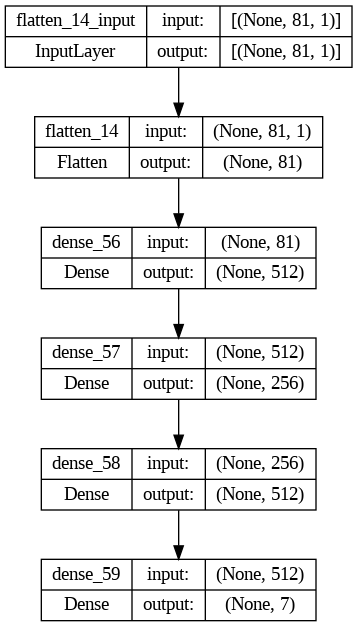
\includegraphics[width=0.3\linewidth]{Photo/15}
	\caption[مدل MLP]{مدل MLP}
	\label{fig:15}
\end{figure}
بعد از پیاده سازی این مدل نتایج به دست آمده در رابطه با این مدل MLP و همچنین با طی کردن ۱۰۰ تعداد دفعات صورت زیر خواهد بود:
\newline
 \begin{table}[h]
	\centering
	\begin{tabular}{l|ll} 
		\hline
		\multicolumn{1}{|l|}{\lr{Model}} & \multicolumn{1}{l|}{\lr{Accuracy}} & \multicolumn{1}{l|}{\lr{Loss}}  \\ 
		\hline
		\lr{MLP}                     & \multicolumn{1}{l|}{$0.9904305934906006$}                         & $0.08047939091920853 $                        \\ 
	\end{tabular}
	\caption{نتایج MLP} \label{foo2}
\end{table}
\newline
مدل شبکه عصبی چندلایه, نسبتا به دقت خوبی دست می‌یابد. این موضوع با توجه به ماهیت شبکه‌های عصبی قابل پیشبینی بود. این مدل‌ها با تصویر کردن داده‌ها به بعد‌های مختلف می‌توانند بهترین ناحیه جداپذیری برای داده‌ها را پیدا کنند و این وظیفه را بهترین حالت انجام دهند.
البته اگر به ماهیت داده‌ها توجه کنیم, برای سیگنال‌های صوتی بهتر از شبکه‌های عصبی حافظه‌دار همچون LSTM استفاده کنیم.
نمودار آموزش شبکه‌ی عصبی به شکل زیر می‌باشد:‌
حال در ادامه ماتریس پراکندگی مربوط به داده‌های تست و آموزش را رسم می‌کنیم نمای کلی از عملکرد سیستم بر روی داده ها را به نمایش بگذارد.\newline
ماتریس پراکندگی بر روی داده های آموزش و تست به صورت زیر به دست می آید:
\newpage
\begin{figure}[h]
	\centering
	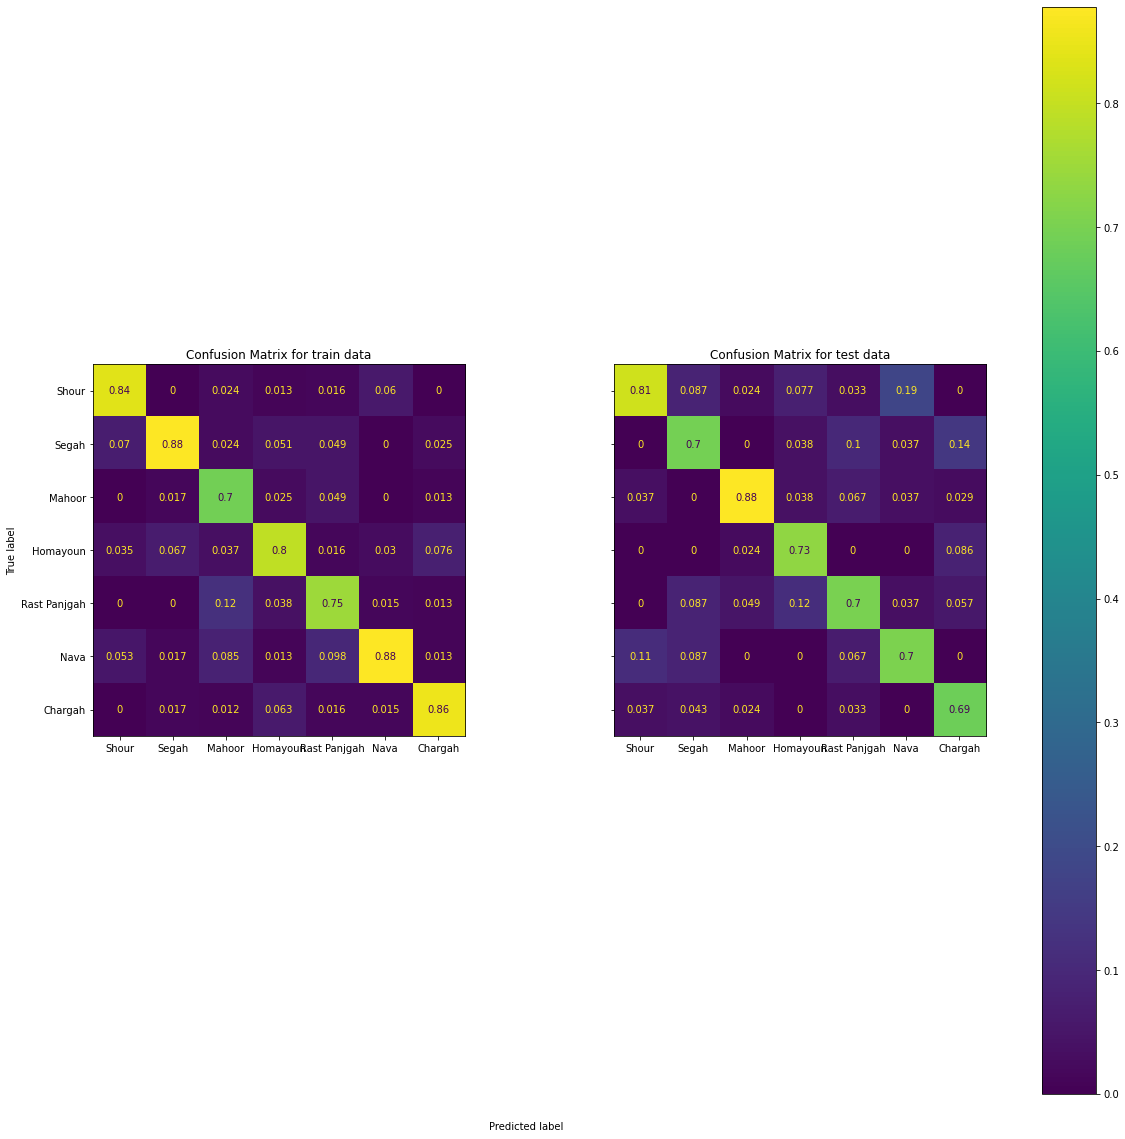
\includegraphics[width=0.7\linewidth]{Photo/111}
	\caption[ماتریس پراکندگی MLP]{ماتریس پراکندگی MLP}
	\label{fig:111}
\end{figure}
ماتریس پراکندگی بهتر نحوه‌ی تقسیم‌بندی کلاس‌ها را نشان می‌دهد. برای مثال در بعضی از کلاس‌ها که تا حدی شبیه هم هستند شبکه اشتباهات بیشتری نسبت به سایر کلاس‌ها انجام می‌دهد.

\subsection{۴-۲) SVM}
به طورکلی \lr{Support vector machines(SVM)} مجموعه‌ای از روش‌های یادگیری تحت نظارت (\lr{supervised}) هستند که برای طبقه‌بندی، رگرسیون استفاده می‌شوند. همه اینها وظایف رایج در یادگیری ماشین هستند.\newline
انواع خاصی از SVM ها وجود دارد که می توانید برای مشکلات خاص یادگیری ماشین استفاده کنید، مانند \lr{support vector regression} (SVR) که توسعه \rl{support vector classification } (SVC) است.\newline
در SVM ها با سایر الگوریتم‌های طبقه‌بندی متفاوت هستند، زیرا آنها مرز تصمیم را انتخاب می‌کنند که فاصله از نزدیک‌ترین نقاط داده همه کلاس‌ها را به حداکثر می‌رساند. \newline
نحوه‌ی عملکرد کلی SVM به این صورت است که با استفاده از کرنل‌هایی داده‌ها را به بعدهای دیگری منتقل می‌کند و در این نواحی جدید تقسیم‌بندی را انجام می‌دهد. البته باید توجه داشت که با استفاده از کرنل‌های مختلف نتایج ما فرق خواهد کرد, برای مثال با توجه به نحوه‌ی توزیع داده‌ها مشخص است که برای داده‌های ما به صورت خطی قابل جداسازی نخواهد بود لذا بهتر است از کرنل‌هایی مانند RBF و Poly استفاده کنیم.

\begin{figure}[h]
	\centering
	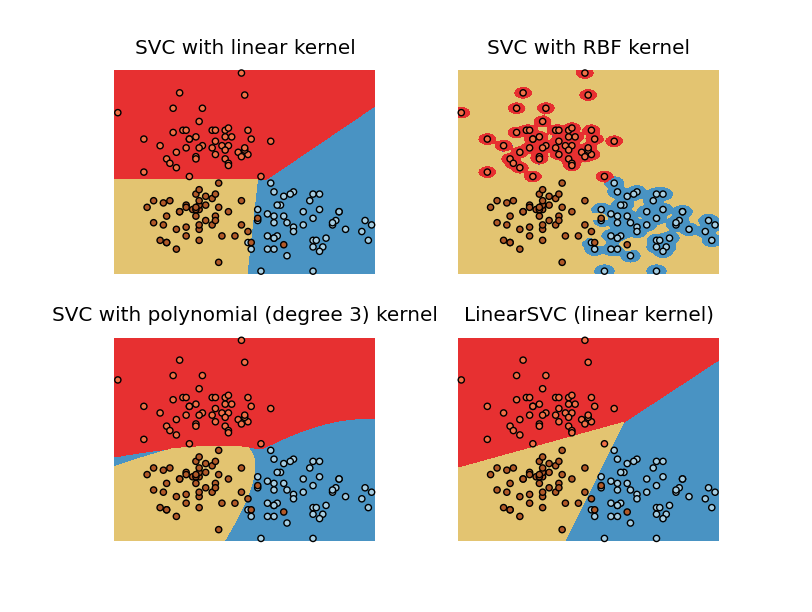
\includegraphics[width=1\linewidth]{Photo/19}
	\caption[کرنل های مختلف \lr{SVM}]{کرنل های مختلف \lr{SVM}}
	\label{fig:16}
\end{figure}
پیش از آن که در مورد مدل پیاده سازی شده صحبت کنیم باید اشنایی نسبی در مورد دو روش \lr{One-VS-One} و \lr{One-VS-All} داشته باشیم که به صورت خلاصه در مورد آن صحبت می کنیم.\newline


۱)\lr{\textbf{One-VS-All}} :می‌توانیم One-Vs-Rest (OvR) یا One-Vs-All (OvA) را به عنوان رویکردی برای ساختن الگوریتم‌های طبقه‌بندی باینری که قادر به کار به عنوان الگوریتم‌های طبقه‌بندی چند کلاسه هستند، در نظر بگیریم. این رویکرد عمدتاً داده های چند کلاسه را به عنوان داده های طبقه بندی باینری تقسیم می کند تا الگوریتم های طبقه بندی باینری را بتوان برای تبدیل داده های طبقه بندی باینری اعمال کرد.\newline


۲)\lr{\textbf{One-VS-One}} :این روش همچنین می تواند به عنوان رویکردی برای ساخت الگوریتم های طبقه بندی باینری با قابلیت کار به عنوان الگوریتم های طبقه بندی چند کلاسه در نظر گرفته شود. این روش مشابه روش One-Vs-Rest است زیرا بر اساس تقسیم داده ها نیز کار می کند، اما رفتار تقسیم این روش به این صورت است. متفاوت از روش One-Vs-Rest. این روش شامل تقسیم داده ها برای هر کلاس است که در آن هر کلاس هر کلاس دیگری را به عنوان حریف خود دارد. ما دوباره می توانیم از مجموعه داده های عنبیه برای درک رفتار تقسیم داده های این روش استفاده کنیم.\newline

در این بخش شکل های مختلفی از SVM را پیده سازی می کنیم و نتایج مربوط به هر کدام را به صورت جداگانه مورد بررسی قرار می دهیم:\newline
۱)\lr{Linear SVM One-Vs-Rest}\newline
۲)\lr{Linear SVM One-Vs-One}\newline
۳)\lr{rbf SVM (gamma=0.7)}\newline
۴)\lr{poly SVM (dgree=3)}\newline


حال نتایج هر کدام از این مدل ها را به صورت جداگانه بر روی دیتاست خود یا به عبارتی بر روی داده های test و train به صورت جداگانه مورد بررسی قرار می دهیم مورد بررسی قرار می دهیم که به صورت زیر تعریف می شوند.\newline

نتایج \lr{Linear SVM One-Vs-Rest} بر روی دیتای train


\begin{table}[h]
	\centering
	\scalebox{0.9}{
	\begin{tabular}{l|l|l|l|l|}
		& \lr{precision} & \lr{recall} & \lr{f1-score} & \lr{support}  \\ 
		\hline
		شور          &$ 0.95$      & $0.83$   & $0.88$     &$ 69$       \\ 
		\hline
		سه گاه       & $1.00  $    &$ 0.97 $  & $0.98   $  &$ 61 $      \\ 
		\hline
		ماهور        &$ 0.94  $    & $0.88 $  &$ 0.91 $    &$ 83 $      \\ 
		\hline
		همایون       &$ 0.85 $     &$ 0.84$   &$ 0.84 $    &$ 81 $      \\ 
		\hline
		راست پنج گاه &$ 0.84  $    &$ 0.96$   &$ 0.9 $     &$ 56 $      \\ 
		\hline
		نوا          &$ 0.81 $     &$ 0.88 $  &$ 0.84 $    & $67 $      \\ 
		\hline
		چهار گاه     &$ 0.9 $      &$ 0.94$   & $0.92 $    &$ 68  $     \\ 
		\hline
		&           &        &          &          \\
		\lr{Accuracy}     &           &        &$ 0.89$     & $485$      \\ 
		\hline
		\lr{macro avg}    &$ 0.9    $   &$ 0.9 $   &$ 0.9  $    &$ 485  $    \\ 
		\hline
		\lr{weighted avg} & $0.9   $    & $0.89 $  & $0.9  $    & $485   $   \\
		\hline
	\end{tabular}}
	\caption{ نتایج \lr{Linear SVM One-Vs-Rest} بر روی دیتای train} \label{foo3}
\end{table}

نتایج \lr{Linear SVM One-Vs-Rest} بر روی دیتای test
\newpage
\begin{table}[h]
	\centering
	\scalebox{0.9}{
	\begin{tabular}{l|l|l|l|l|}
		& \lr{precision} & \lr{recall} & \lr{f1-score} & \lr{support}  \\ 
		\hline
		شور          &$0.41$    & $0.29$   & $0.34$     &$ 41$       \\ 
		\hline
		سه گاه       & $0.26 $    &$ 0.35$  & $0.30   $  &$26 $      \\ 
		\hline
		ماهور        &$ 0.32 $    & $0.23$  &$ 0.26$    &$ 40 $      \\ 
		\hline
		همایون       &$ 0.17$     &$ 0.15$   &$ 0.16 $    &$ 27 $      \\ 
		\hline
		راست پنج گاه &$ 0.14 $   &$ 0.19$   &$ 0.16$     &$ 21$      \\ 
		\hline
		نوا          &$ 0.23$     &$ 0.23 $  &$ 0.23 $    & $30 $      \\ 
		\hline
		چهار گاه     &$ 0.35$      &$ 0.5$   & $0.41 $    &$ 24  $     \\ 
		\hline
		&           &        &          &          \\
		\lr{Accuracy}     &           &        &$ 0.27$     & $209$      \\ 
		\hline
		\lr{macro avg}    &$ 0.27    $   &$ 0.28 $   &$ 0.27 $    &$ 209  $    \\ 
		\hline
		\lr{weighted avg} & $0.28   $    & $0.27 $  & $0.27  $    & $209   $   \\
		\hline
	\end{tabular}}
	\caption{ نتایج \lr{Linear SVM One-Vs-Rest} بر روی دیتای test} \label{foo4}
\end{table}
نتایج \lr{Linear SVM One-Vs-One} بر روی دیتای train

\begin{table}[h]
	\centering
	\scalebox{0.9}{
	\begin{tabular}{l|l|l|l|l|}
		& \lr{precision} & \lr{recall} & \lr{f1-score} & \lr{support}  \\ 
		\hline
		شور          &$0.47$    & $0.51$   & $0.49$     &$55$       \\ 
		\hline
		سه گاه       & $0.81 $    &$ 0.66$  & $0.73   $  &$73$      \\ 
		\hline
		ماهور        &$ 0.69 $    & $0.67$  &$ 0.68$    &$ 81$      \\ 
		\hline
		همایون       &$ 0.55$     &$ 0.63$   &$ 0.59$    &$ 70 $      \\ 
		\hline
		راست پنج گاه &$ 0.55$   &$ 0.60$   &$ 0.67$     &$ 58$      \\ 
		\hline
		نوا          &$ 0.60$     &$ 0.62 $  &$ 0.61 $    & $71 $      \\ 
		\hline
		چهار گاه     &$ 0.73$      &$ 0.68$   & $0.70 $    &$ 77 $     \\ 
		\hline
		&           &        &          &          \\
		\lr{Accuracy}     &           &        &$ 0.63$     & $485$      \\ 
		\hline
		\lr{macro avg}    &$ 0.63    $   &$ 0.62 $   &$ 0.62 $    &$ 485  $    \\ 
		\hline
		\lr{weighted avg} & $0.64   $    & $0.63 $  & $0.63  $    & $485   $   \\
		\hline
	\end{tabular}}
	\caption{ نتایج \lr{Linear SVM One-Vs-One} بر روی دیتای train} \label{foo5}
\end{table}


نتایج \lr{Linear SVM One-Vs-One} بر روی دیتای test
\newpage


\begin{table}[h]
	\centering
	\scalebox{0.9}{
		\begin{tabular}{l|l|l|l|l|}
			& \lr{precision} & \lr{recall} & \lr{f1-score} & \lr{support}  \\ 
			\hline
			شور          &$0.24$    & $0.27$   & $0.25$     &$26$       \\ 
			\hline
			سه گاه       & $0.31 $    &$ 0.33$  & $0.32   $  &$33$      \\ 
			\hline
			ماهور        &$ 0.29 $    & $0.21$  &$ 0.24$    &$ 38$      \\ 
			\hline
			همایون       &$ 0.17$     &$ 0.17$   &$ 0.17$    &$ 24 $      \\ 
			\hline
			راست پنج گاه &$ 0.18$   &$ 0.19$   &$ 0.19$     &$ 26$      \\ 
			\hline
			نوا          &$ 0.26$     &$ 0.26 $  &$ 0.26 $    & $31 $      \\ 
			\hline
			چهار گاه     &$ 0.38$      &$ 0.42$   & $0.40 $    &$ 31 $     \\ 
			\hline
			&           &        &          &          \\
			\lr{Accuracy}     &           &        &$ 0.27$     & $209$      \\ 
			\hline
			\lr{macro avg}    &$ 0.26    $   &$ 0.26 $   &$ 0.26 $    &$ 209  $    \\ 
			\hline
			\lr{weighted avg} & $0.27   $    & $0.27 $  & $0.27  $    & $209   $   \\
			\hline
	\end{tabular}}
	\caption{ نتایج \lr{Linear SVM One-Vs-One} بر روی دیتای test} \label{foo6}
\end{table}

نتایج \lr{rbf SVM } بر روی دیتای train


\begin{table}[h]
	\centering
	\scalebox{0.9}{
		\begin{tabular}{l|l|l|l|l|}
			& \lr{precision} & \lr{recall} & \lr{f1-score} & \lr{support}  \\ 
			\hline
			شور          &$1$    & $1$   & $1$     &$65$       \\ 
			\hline
			سه گاه       & $1 $    &$ 1$  & $1   $  &$59$      \\ 
			\hline
			ماهور        &$ 1 $    & $1$  &$ 1$    &$ 78$      \\ 
			\hline
			همایون       &$ 1$     &$ 1$   &$ 1$    &$ 80 $      \\ 
			\hline
			راست پنج گاه &$ 1$   &$ 1$   &$ 1$     &$ 64$      \\ 
			\hline
			نوا          &$ 1$     &$ 1 $  &$ 1 $    & $73 $      \\ 
			\hline
			چهار گاه     &$ 1$      &$ 1$   & $1 $    &$ 71 $     \\ 
			\hline
			&           &        &          &          \\
			\lr{Accuracy}     &           &        &$ 1$     & $485$      \\ 
			\hline
			\lr{macro avg}    &$ 1    $   &$ 1 $   &$ 1 $    &$ 485  $    \\ 
			\hline
			\lr{weighted avg} & $1   $    & $1 $  & $1  $    & $485   $   \\
			\hline
	\end{tabular}}
	\caption{ نتایج \lr{rbf SVM } بر روی دیتای train} \label{foo7}
\end{table}


نتایج \lr{rbf SVM } بر روی دیتای test
\newpage
\begin{table}[h]
	\centering
	\scalebox{0.9}{
		\begin{tabular}{l|l|l|l|l|}
			& \lr{precision} & \lr{recall} & \lr{f1-score} & \lr{support}  \\ 
			\hline
			شور          &$0.03$    & $1$   & $0.07$     &$1$       \\ 
			\hline
			سه گاه       & $0.03 $    &$1$  & $0.06   $  &$1$      \\ 
			\hline
			ماهور        &$ 0.04 $    & $0.50$  &$ 0.07$    &$ 2$      \\ 
			\hline
			همایون       &$ 0.96$     &$ 0.11$   &$ 0.20$    &$ 203 $      \\ 
			\hline
			راست پنج گاه &$ 0.07$   &$1$   &$ 0.13$     &$ 2$      \\ 
			\hline
			نوا          &$ 0.00$     &$ 0.00 $  &$ 0.00 $    & $0 $      \\ 
			\hline
			چهار گاه     &$ 0.00$      &$ 0.00$   & $0.00 $    &$ 0 $     \\ 
			\hline
			&           &        &          &          \\
			\lr{Accuracy}     &           &        &$ 0.13$     & $209$      \\ 
			\hline
			\lr{macro avg}    &$ 0.16    $   &$ 0.52 $   &$ 0.07 $    &$ 209  $    \\ 
			\hline
			\lr{weighted avg} & $0.93   $    & $0.13 $  & $0.20  $    & $209   $   \\
			\hline
	\end{tabular}}
	\caption{نتایج \lr{rbf SVM } بر روی دیتای test} \label{foo8}
\end{table}


نتایج \lr{poly SVM } بر روی دیتای train
\begin{table}[h]
	\centering
	\scalebox{0.9}{
		\begin{tabular}{l|l|l|l|l|}
			& \lr{precision} & \lr{recall} & \lr{f1-score} & \lr{support}  \\ 
			\hline
			شور          &$0.58$    & $1$   & $0.74$     &$35$       \\ 
			\hline
			سه گاه       & $0.56 $    &$ 1$  & $0.72   $  &$33$      \\ 
			\hline
			ماهور        &$ 0.95 $    & $0.93$  &$ 0.94$    &$ 80$      \\ 
			\hline
			همایون       &$ 0.93$     &$ 0.95$   &$ 0.94$    &$ 78 $      \\ 
			\hline
			راست پنج گاه &$ 0.75$   &$ 1$   &$ 0.86$     &$ 48$      \\ 
			\hline
			نوا          &$ 1$     &$ 0.47 $  &$ 0.64 $    & $155 $      \\ 
			\hline
			چهار گاه     &$ 0.79$      &$1$   & $0.88 $    &$ 56 $     \\ 
			\hline
			&           &        &          &          \\
			\lr{Accuracy}     &           &        &$ 0.81$     & $485$      \\ 
			\hline
			\lr{macro avg}    &$ 0.79    $   &$ 0.91 $   &$ 0.82 $    &$ 485  $    \\ 
			\hline
			\lr{weighted avg} & $0.87   $    & $0.81 $  & $0.80  $    & $485   $   \\
			\hline
	\end{tabular}}
	\caption{ نتایج \lr{poly SVM } بر روی دیتای train} \label{foo9}
\end{table}


نتایج \lr{poly SVM } بر روی دیتای test
\newpage
\begin{table}[h]
	\centering
	\scalebox{0.9}{
		\begin{tabular}{l|l|l|l|l|}
			& \lr{precision} & \lr{recall} & \lr{f1-score} & \lr{support}  \\ 
			\hline
			شور          &$0.17$    & $0.71$   & $0.28$     &$7$       \\ 
			\hline
			سه گاه       & $0.03 $    &$ 0.33$  & $0.05   $  &$3$      \\ 
			\hline
			ماهور        &$ 0.43 $    & $0.30$  &$ 0.35$    &$ 40$      \\ 
			\hline
			همایون       &$ 0.12$     &$ 0.15$   &$ 0.14$    &$ 20 $      \\ 
			\hline
			راست پنج گاه &$ 0.14$   &$ 0.44$   &$ 0.22$     &$ 9$      \\ 
			\hline
			نوا          &$ 0.81$     &$ 0.22 $  &$ 0.35 $    & $113 $      \\ 
			\hline
			چهار گاه     &$ 0.35$      &$ 0.71$   & $0.47 $    &$ 17 $     \\ 
			\hline
			&           &        &          &          \\
			\lr{Accuracy}     &           &        &$ 0.30$     & $209$      \\ 
			\hline
			\lr{macro avg}    &$ 0.29    $   &$ 0.41 $   &$ 0.26 $    &$ 209  $    \\ 
			\hline
			\lr{weighted avg} & $0.57   $    & $0.30 $  & $0.33  $    & $209   $   \\
			\hline
	\end{tabular}}
	\caption{نتایج \lr{poly SVM } بر روی دیتای test} \label{foo10}
\end{table}

همان طور که مشاهده می‌شود نتایج برای تقریبا همه SVM‌ها روی train  قابل قبول است ولی به همان ترتیب بر روی داده‌های تست نتایج بهترین حالت نیست. اگر بخواهیم نتایج هر یک از چهار مدل را به صورت جداگانه بر روی داده‌های آموزش مورد بررسی قرار دهیم باید اشاره کرد, همان طور که از قبل پیشبینی نیز می‌شد بدترین نتیجه را svm خطی OvO برای ما به دست می آورد زیرا توانای لازم برای طبقه بنده داده‌های ما با توجه به ویژگی هایی که پیشتر لحاظ کردیم را ندارد و در محاسبات خود برای طبقه بندی از ساختار ساده تری استفاده می کند در ادامه البته باید اشاره کرد که svm خطی OvR بر روی داده‌های آموزش نتیجه به مراتب بهتری به ما ارایه می دهد.\newline
 در ادامه شایان ذکر است که \lr{poly svm} بر روی داده های train عملکردی مشابه svm خطی OvR دارد و تفاوت چندانی با هم پیدا نمی کند و تفاوتی که دارند در قالب مقایسه قبل اغماض است ولی \lr{rbf svm} بر روی داده های train ما overfit می کند و دقت ۱۰۰ درصد را به ما ارایه می دهد که بهترین دقت در میان چهار مدل train شده است.\newline
حال که هر چهار مدل را بر روی داده های train بررسی کردیم باید دست آورد هر کدام را بر روی داده های test مورد بررسی قرار دهیم تا ببنیم میزان اعتمادی که به هر مدل می توان کرد در چه اندازه ای خواهد بود.برای شروع می توان گفت که نسبت به بخش قبل به طورکلی svm نتایج به مراتب ضعیف تری در اختیار ما قرار خواهد داد.\newline
بدترین نتیجه همان طور که در بند قبل گفتیم با مشاهده overfit در مدل \lr{rbf svm} به این مدل اختصاص پیدا می کند و دقت بسار پایینی بر روی داده های test در اختیار ما قرار می دهد.\newline
از بین سه مدل باقی مانده می توان گفت که هر سه تای آن ها یعنی \lr{poly svm} , svm خطی OvO و svm خطی OvR دقت تقریبا برابری بر روی داده های تست از خود نشان می دهند نسبت به یکدیگر برتری نشان نمی دهند هر چند که کماکان دقت خوبی در اختیار ما قرار نمی دهند و در یک نتیجه گیری کلی تمامی مدل های train شده svm در این گزارش از MLP عملکرد بدتری بر روی داده های تست به نمایش در می آورند.



حال برای فهم بهتر از خروجی چهار مدل خود می توانیم از ماتریس پراکندگی استقاده کنیم که نتایج بهتر را برای فهم قضیه در اختیار ما قرار می دهد.\newline
\begin{figure}[h]
	\centering
	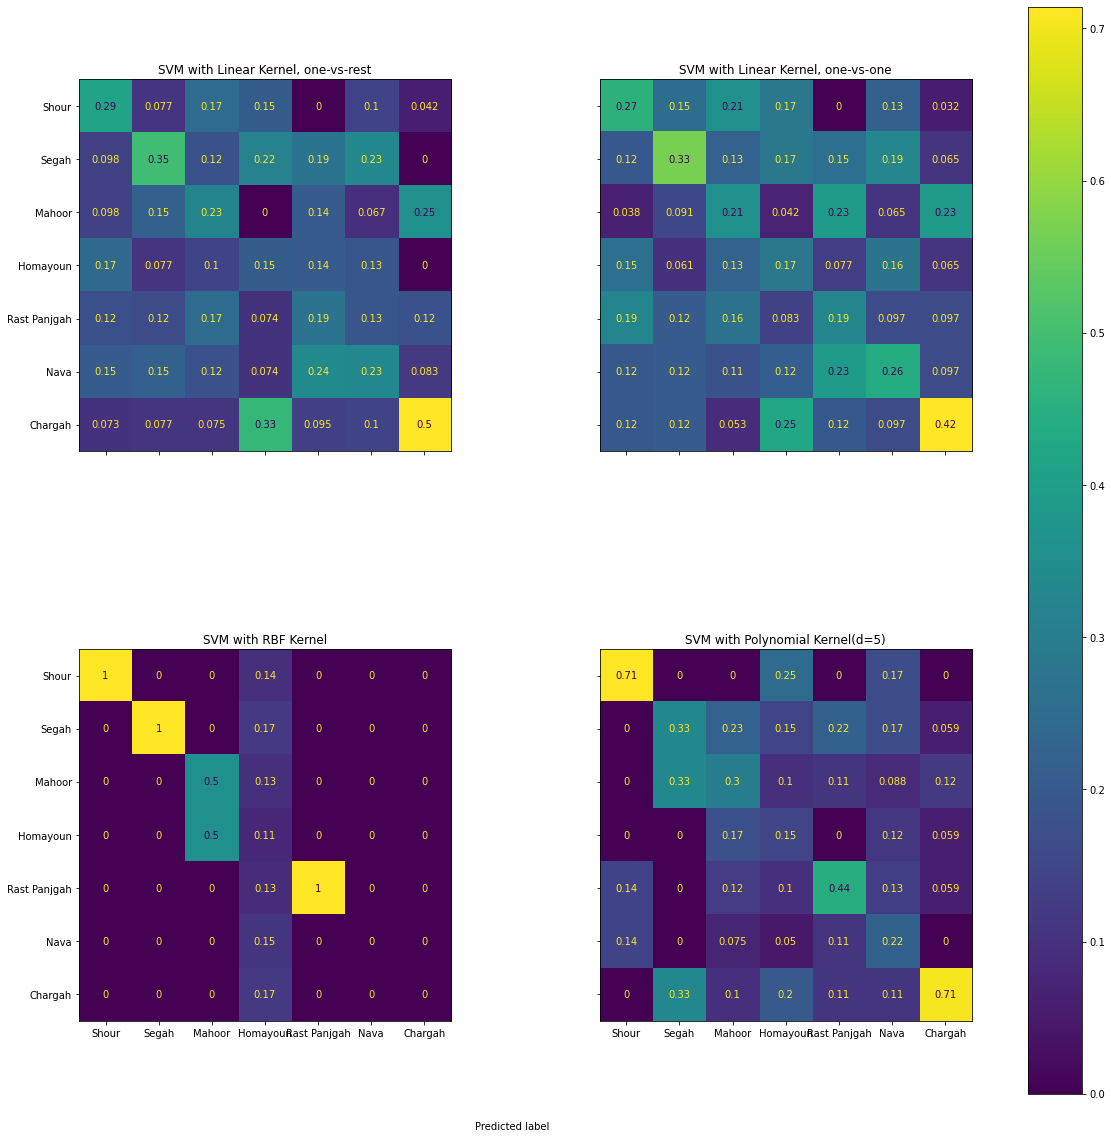
\includegraphics[width=0.7\linewidth]{Photo/20}
	\caption[ماتریس پراکندگی \lr{svm} ها]{ماتریس پراکندگی \lr{svm} ها}
	\label{fig:20}
\end{figure}


\subsection{۴-۳) Knn}
الگوریتم \lr{ K-Nearest Neighbors} همچنین به عنوان KNN یا k-NN شناخته می شود، یک طبقه بندی کننده یادگیری \lr{non-parametric} و \lr{supervised} است که از تقریب نزدیکی نقاط برای انجام طبقه بندی یا پیش بینی در مورد گروه بندی یک نقطه داده فردی استفاده می کند.\newline
در حالی که می‌توان از آن برای مسائل رگرسیون یا طبقه‌بندی استفاده کرد، معمولاً به عنوان یک الگوریتم طبقه‌بندی استفاده می‌شود، با این فرض که نقاط مشابه را می‌توان در نزدیکی یکدیگر یافت.\newline
برای مسایل طبقه بندی، یک label کلاس بر اساس رای اکثریت اختصاص داده می شود به عبارتی برچسبی (label) که بیشتر از بقیه در اطراف یک نقطه داده شده معین نشان داده می شود مورد استفاده قرار می گیرد. در حالی که این از نظر فنی "رای گیری کثرت" در نظر گرفته می شود، اصطلاح "رای اکثریت" بیشتر در ادبیات استفاده می شود.
\newpage
\begin{figure}[h]
	\centering
	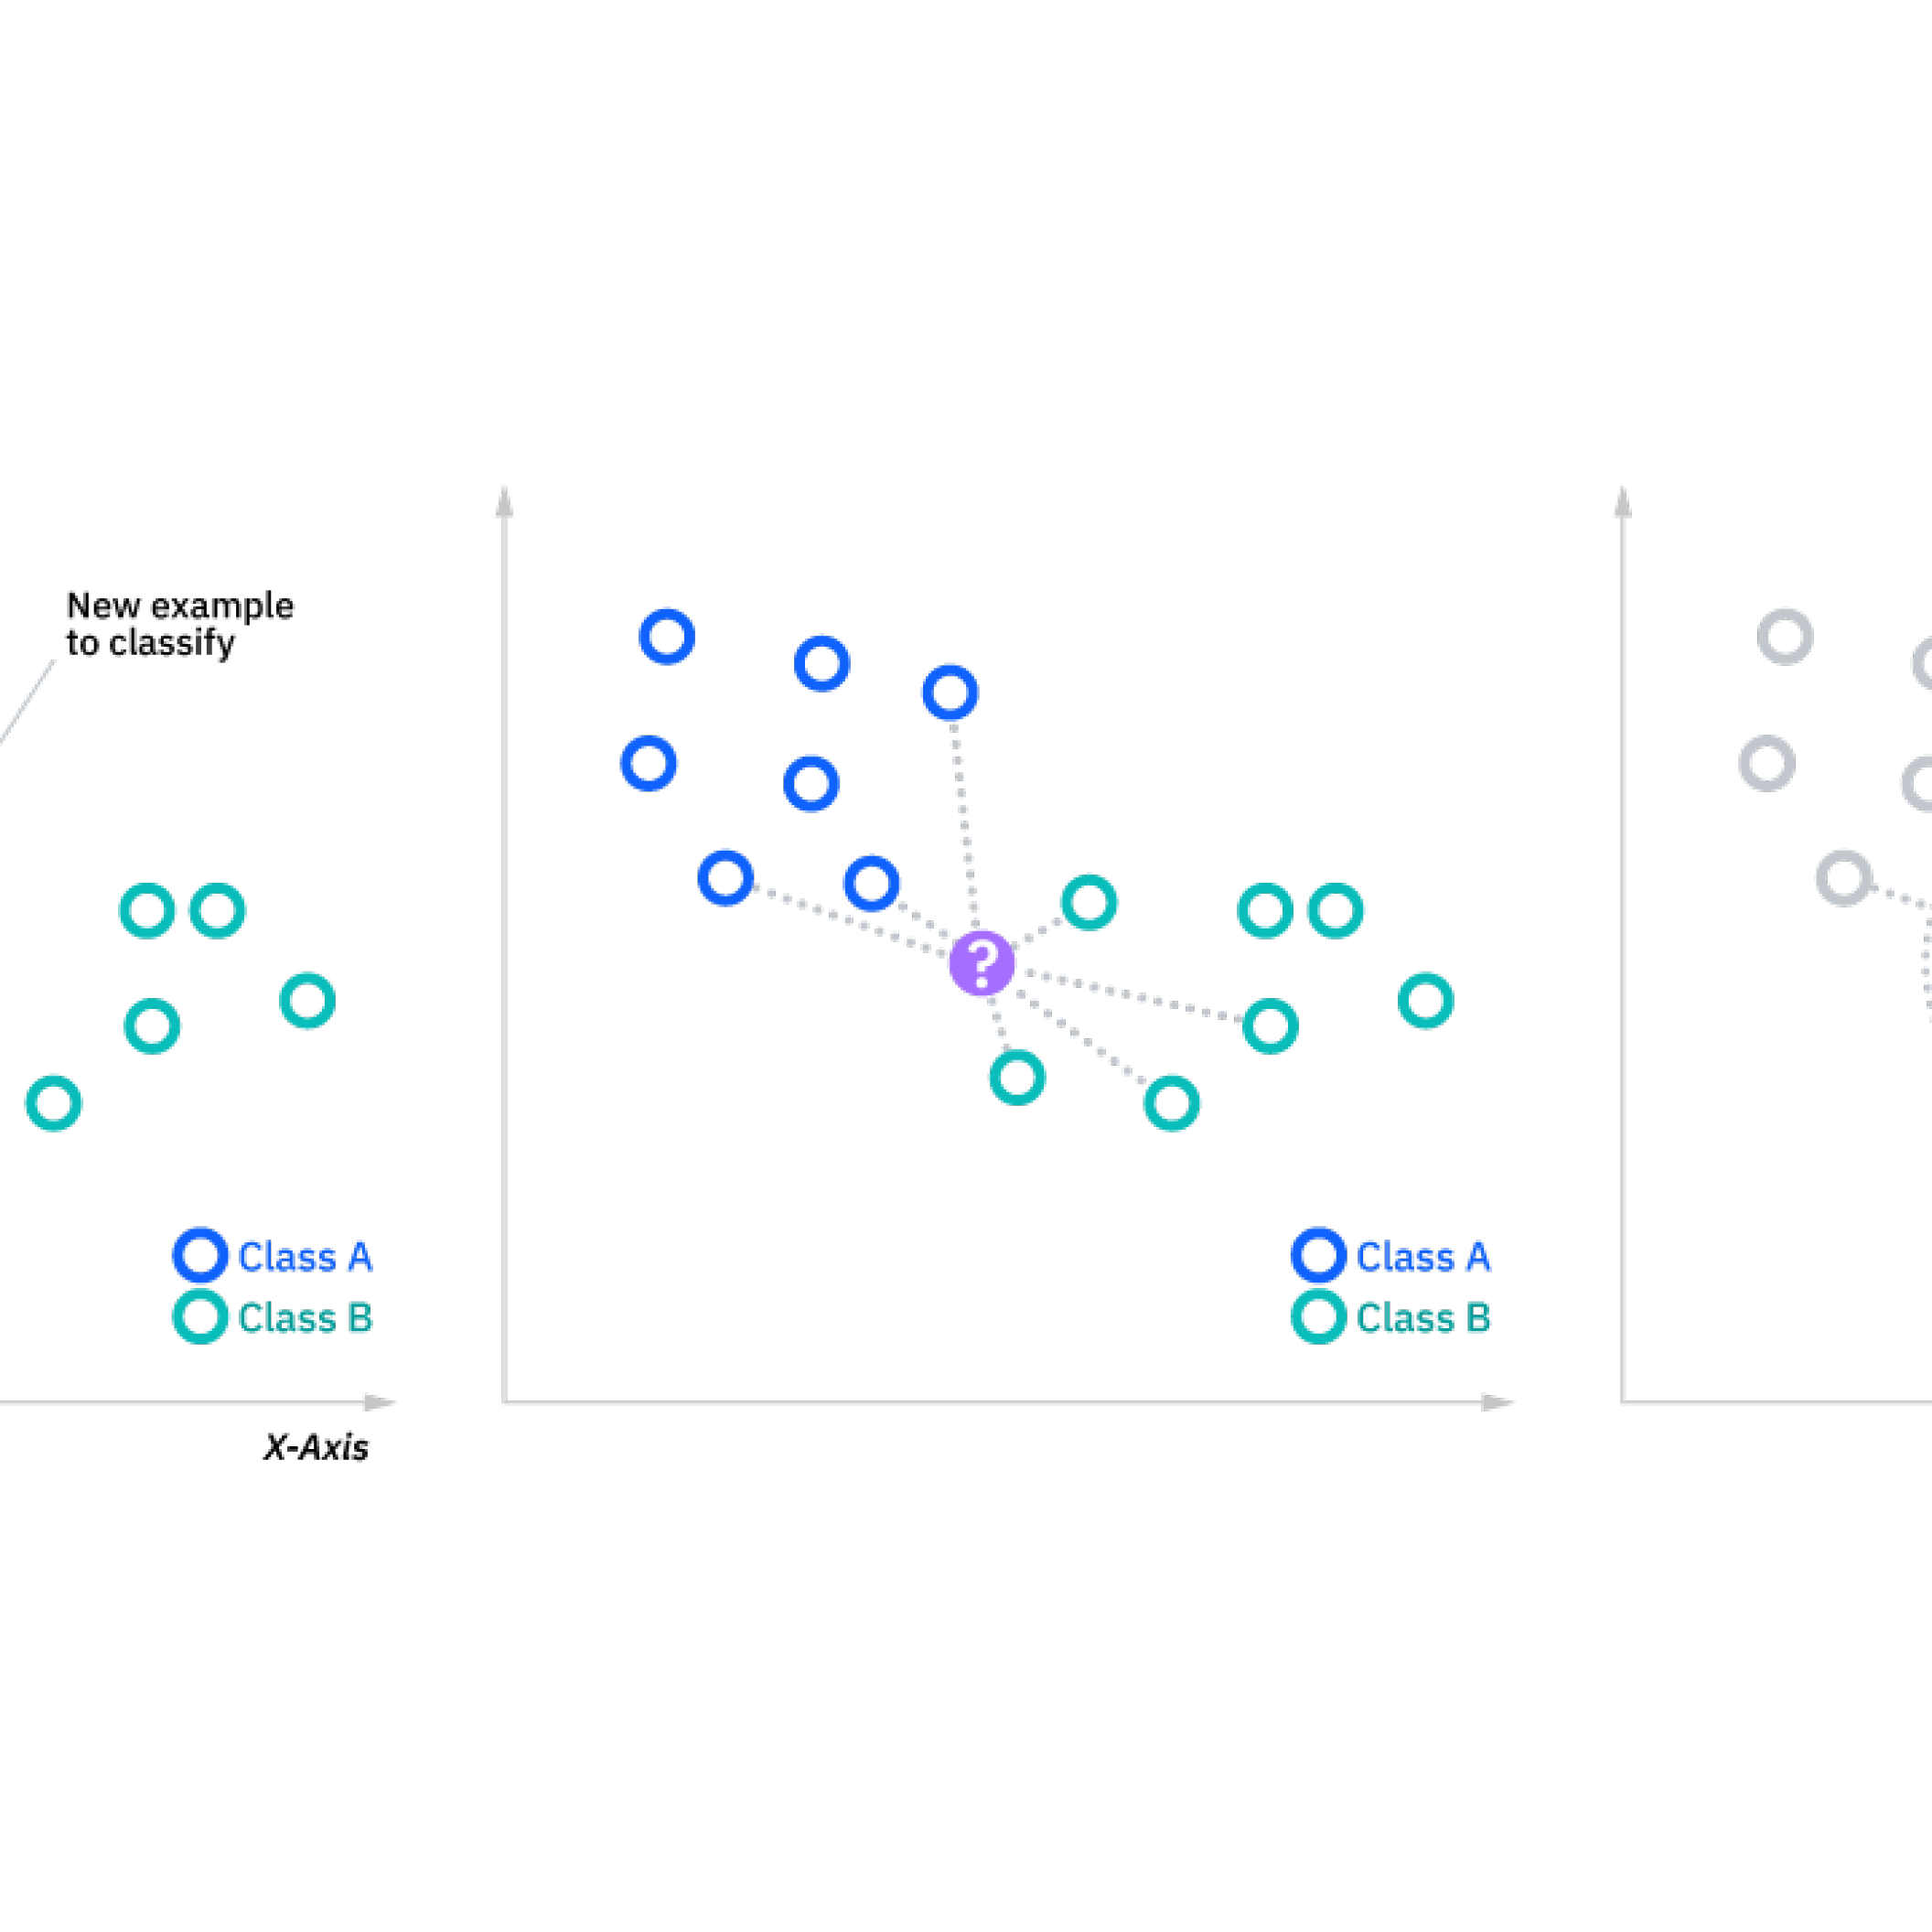
\includegraphics[width=0.5\linewidth]{Photo/21}
	\caption[روش محاسباتی \lr{knn}]{روش محاسباتی \lr{knn}}
	\label{fig:21}
\end{figure}
حال ما مدل knn خود را با تعداد همسایگی های ۵ پیاده سازی می کنیم.\newline
دقت مدل knn ما بر روی داده های train به صورت جدول زیر به دست می آید:\newline
\begin{table}[h]
	\centering
	\scalebox{0.8}{
		\begin{tabular}{l|l|l|l|l|}
			& \lr{precision} & \lr{recall} & \lr{f1-score} & \lr{support}  \\ 
			\hline
			شور          &$0.67$    & $0.44$   & $0.53$     &$86$       \\ 
			\hline
			سه گاه       & $0.65 $    &$ 0.54$  & $0.59   $  &$74$      \\ 
			\hline
			ماهور        &$ 0.63 $    & $0.58$  &$ 0.61$    &$ 74$      \\ 
			\hline
			همایون       &$ 0.50$     &$ 0.66$   &$ 0.57$    &$ 59 $      \\ 
			\hline
			راست پنج گاه &$ 0.57$   &$ 0.67$   &$ 0.62$     &$60$      \\ 
			\hline
			نوا          &$ 0.61$     &$ 0.61 $  &$ 0.61 $    & $76 $      \\ 
			\hline
			چهار گاه     &$ 0.57$      &$ 0.77$   & $0.66 $    &$ 56 $     \\ 
			\hline
			&           &        &          &          \\
			\lr{Accuracy}     &           &        &$ 0.60$     & $485$      \\ 
			\hline
			\lr{macro avg}    &$ 0.60    $   &$ 0.61 $   &$ 0.60 $    &$ 485  $    \\ 
			\hline
			\lr{weighted avg} & $0.61   $    & $0.60 $  & $0.59  $    & $485   $   \\
			\hline
	\end{tabular}}
	\caption{نتایج \lr{Knn} بر روی دیتای train} \label{foo11}
\end{table}
همچنین دقت مدل knn ما بر روی داده های test به صورتی زیر به دست می آید:
\newline
\newpage
\begin{table}[h]
	\centering
	\scalebox{0.8}{
		\begin{tabular}{l|l|l|l|l|}
			& \lr{precision} & \lr{recall} & \lr{f1-score} & \lr{support}  \\ 
			\hline
			شور          &$0.16$    & $0.15$   & $0.15$     &$34$       \\ 
			\hline
			سه گاه       & $0.31 $    &$ 0.33$  & $0.32   $  &$30$      \\ 
			\hline
			ماهور        &$ 0.50 $    & $0.50$  &$ 0.50$    &$ 38$      \\ 
			\hline
			همایون       &$ 0.19$     &$ 0.17$   &$ 0.18$    &$ 29 $      \\ 
			\hline
			راست پنج گاه &$ 0.32$   &$ 0.35$   &$ 0.33$     &$20$      \\ 
			\hline
			نوا          &$ 0.38$     &$ 0.35 $  &$ 0.37 $    & $31 $      \\ 
			\hline
			چهار گاه     &$ 0.50$      &$ 0.56$   & $0.53 $    &$ 27 $     \\ 
			\hline
			&           &        &          &          \\
			\lr{Accuracy}     &           &        &$ 0.34$     & $209$      \\ 
			\hline
			\lr{macro avg}    &$ 0.34    $   &$ 0.34 $   &$ 0.34 $    &$ 209  $    \\ 
			\hline
			\lr{weighted avg} & $0.34   $    & $0.34 $  & $0.34  $    & $209   $   \\
			\hline
	\end{tabular}}
	\caption{نتایج \lr{Knn} بر روی دیتای test} \label{foo12}
\end{table}
همان طور که مشاهده می شود دقت نهایی این مدل knn نسبت به svm ها بهتر است و در حدود ۳۴ درصد قرار می گیرد ون نتایج بهتری را در رابطه با طبقه بندی در اختیار ما قرار می دهد که در جدول بالا کاملا قبل مشاهده است.همچنین برای درک بهتر این مدل ماتریس پراکندگی آن به صورت زیر به دست می آید.
\begin{figure}[h]
	\centering
	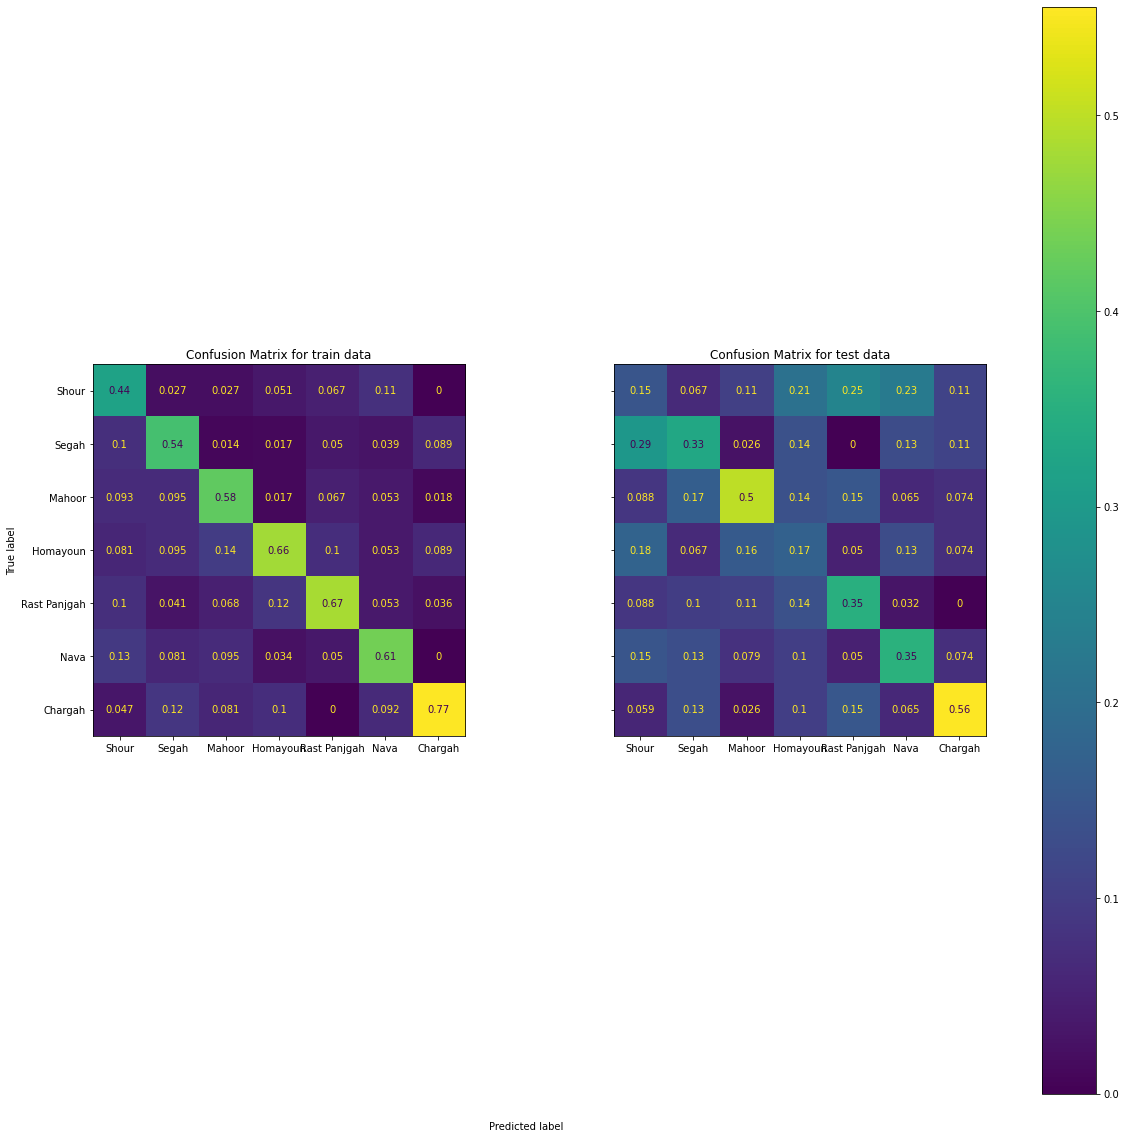
\includegraphics[width=0.5\linewidth]{Photo/22}
	\caption[ماتریس پراکندگی مدل \lr{knn}]{ماتریس پراکندگی مدل \lr{knn}}
	\label{fig:22}
\end{figure}
\newpage

\subsection{۴-۴) \lr{Logistic Regression}}
به طور کلی \lr{Logistic Regression} یک روش تحلیل آماری برای پیش‌بینی یک نتیجه باینری، مانند بله یا خیر، بر اساس مشاهدات قبلی یک مجموعه داده است.
یک مدل \lr{Logistic Regression} با تجزیه و تحلیل رابطه بین یک یا چند متغیر مستقل موجود، یک متغیر داده وابسته را پیش‌بینی می‌کند.
در عمل ر\lr{Logistic Regression} به یک ابزار مهم در رشته یادگیری ماشین تبدیل شده است. \lr{Logistic Regression} به الگوریتم‌های مورد استفاده در برنامه‌های یادگیری ماشین اجازه می‌دهد تا داده‌های دریافتی را بر اساس داده‌های قبلی طبقه‌بندی کنند. با ورود داده های مرتبط اضافی، الگوریتم ها در پیش بینی طبقه بندی در مجموعه داده ها بهتر می شوند.
مانند طبقه بندی کننده های قبل اینبار مدل \lr{Logistic Regression} بر روی داده های خود پیاده سازی می کنیم.\newline
بعد از پیاده سازی مدل نتایج آن بر روی داده های train به صورت زیر گزارش می شود:\newline
\begin{table}[h]
	\centering
	\scalebox{0.8}{
		\begin{tabular}{l|l|l|l|l|}
			& \lr{precision} & \lr{recall} & \lr{f1-score} & \lr{support}  \\ 
			\hline
			شور          &$0.32$    & $0.43$   & $0.36$     &$42$       \\ 
			\hline
			سه گاه       & $0.52 $    &$ 0.49$  & $0.50   $  &$65$      \\ 
			\hline
			ماهور        &$ 0.44 $    & $0.46$  &$ 0.45$    &$ 65$      \\ 
			\hline
			همایون       &$ 0.56$     &$ 0.50$   &$ 0.53$    &$ 88 $      \\ 
			\hline
			راست پنج گاه &$ 0.37$   &$ 0.47$   &$ 0.42$     &$55$      \\ 
			\hline
			نوا          &$ 0.57$     &$ 0.51 $  &$ 0.54 $    & $85 $      \\ 
			\hline
			چهار گاه     &$ 0.57$      &$ 0.51$   & $0.54 $    &$ 85 $     \\ 
			\hline
			&           &        &          &          \\
			\lr{Accuracy}     &           &        &$ 0.49$     & $485$      \\ 
			\hline
			\lr{macro avg}    &$ 0.48    $   &$ 0.48 $   &$ 0.48 $    &$ 485  $    \\ 
			\hline
			\lr{weighted avg} & $0.50   $    & $0.49 $  & $0.49  $    & $485   $   \\
			\hline
	\end{tabular}}
	\caption{نتایج \lr{Logistic Regression} بر روی دیتای train} \label{foo13}
\end{table}


در ادامه همانند قبل مدل را بر روی داده های test پیاده سازی می کنیم نتیجه محکم تری از مدل طراحی شده خود به دست آوریم:
\begin{table}[h]
	\centering
	\scalebox{0.8}{
		\begin{tabular}{l|l|l|l|l|}
			& \lr{precision} & \lr{recall} & \lr{f1-score} & \lr{support}  \\ 
			\hline
			شور          &$0.06$    & $0.14$   & $0.09$     &$14$       \\ 
			\hline
			سه گاه       & $0.34 $    &$ 0.39$  & $0.37   $  &$28$      \\ 
			\hline
			ماهور        &$ 0.26 $    & $0.33$  &$ 0.29$    &$ 30$      \\ 
			\hline
			همایون       &$ 0.27$     &$ 0.20$   &$ 0.23$    &$ 35 $      \\ 
			\hline
			راست پنج گاه &$ 0.18$   &$ 0.15$   &$ 0.17$     &$26$      \\ 
			\hline
			نوا          &$ 0.41$     &$ 0.27 $  &$ 0.33 $    & $44 $      \\ 
			\hline
			چهار گاه     &$ 0.37$      &$ 0.34$   & $0.35 $    &$ 32 $     \\ 
			\hline
			&           &        &          &          \\
			\lr{Accuracy}     &           &        &$ 0.27$     & $209$      \\ 
			\hline
			\lr{macro avg}    &$ 0.27    $   &$ 0.26 $   &$ 0.26 $    &$ 209  $    \\ 
			\hline
			\lr{weighted avg} & $0.30   $    & $0.27 $  & $0.28  $    & $209   $   \\
			\hline
	\end{tabular}}
	\caption{نتایج \lr{Logistic Regression} بر روی دیتای train} \label{foo14}
\end{table}


همان طور که از جدول بالا مشاهده می شود دقت مدل \lr{Logistic Regression} بر روی داده های test در مقایسه با دو طبقه بندی کننده قبلی پایین تر است.\newline
حال برای درک بهتر مدل به دست آمده \lr{Logistic Regression} ماتریس پراکندگی آن را به صورت زیر به دست می آوریم:
\begin{figure}[h]
	\centering
	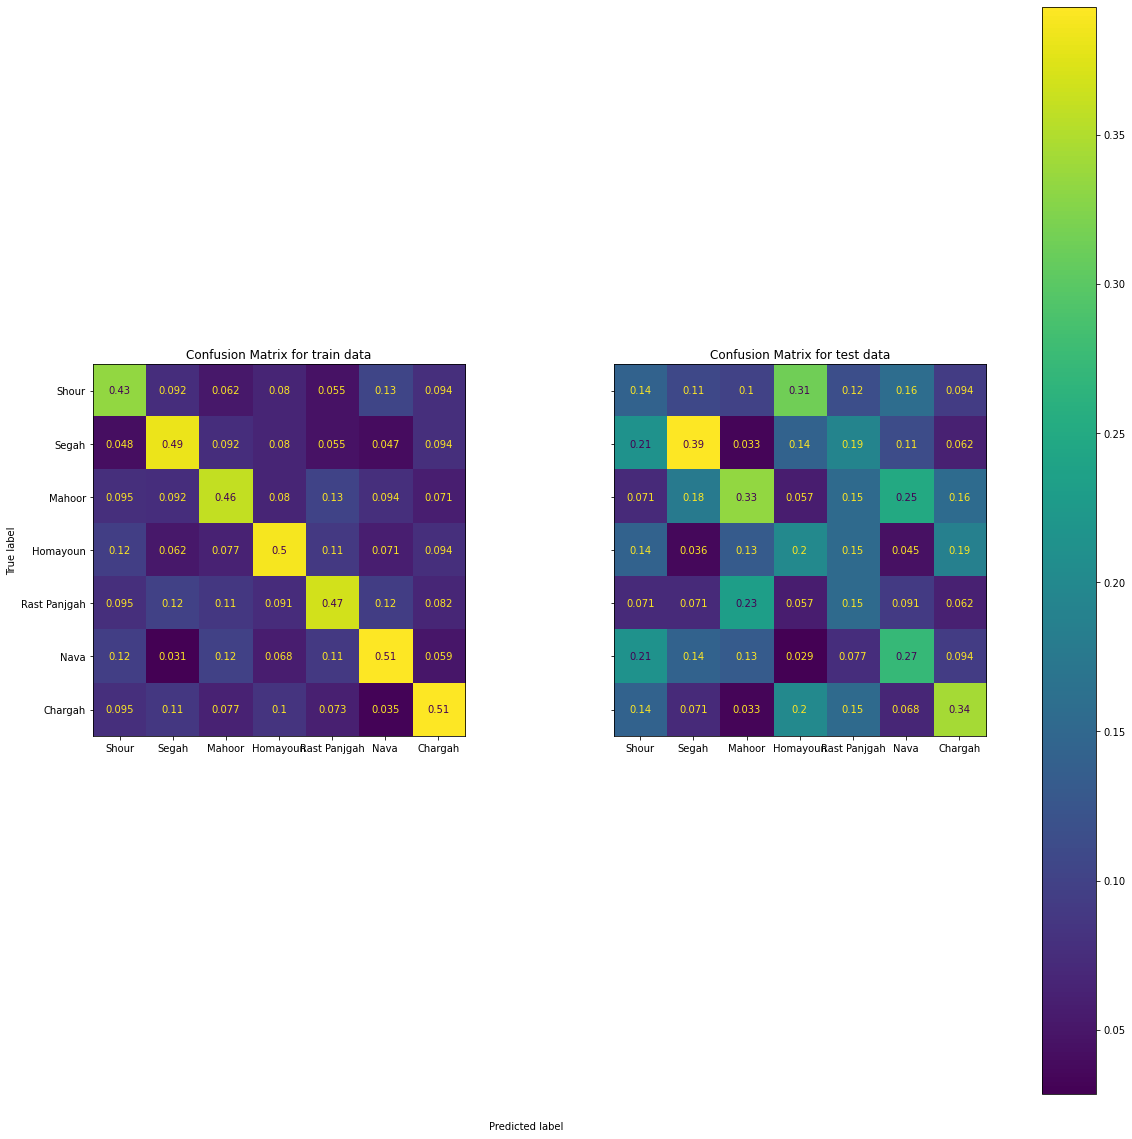
\includegraphics[width=0.7\linewidth]{Photo/23}
	\caption[ماتریس پراکندگی \lr{Logistic Regression} ]{ماتریس پراکندگی \lr{Logistic Regression} }
	\label{fig:23}
\end{figure}

\subsection{۴-۵) \lr{Ensemble Learning}}
یادگیری گروهی \lr{Ensemble Learning} یک رویکرد خوب برای یادگیری ماشینی است که با ترکیب پیش‌بینی‌های چند مدل به دنبال عملکرد پیش‌بینی بهتری است.\newline
اگرچه تعداد به ظاهر نامحدودی از مجموعه‌ها وجود دارد که می‌توانید برای مشکل مدل‌سازی پیش‌بینی‌کننده خود ایجاد کنید، سه روش وجود دارد که بر حوزه یادگیری گروهی \lr{Ensemble Learning} تسلط دارند. به حدی که به جای الگوریتم‌ها فی نفسه، هر یک رشته‌ای هستند که روش‌های تخصصی‌تری را ایجاد کرده‌اند.\newline
او چهار کلاس اصلی از روش‌های یادگیری گروهی عبارتند از: \lr{boosting}, \lr{stacking}, \lr{voting},\lr{bagging} و مهم است که هم درک دقیقی از هر روش داشته باشید و هم آنها را در پروژه مدل‌سازی پیش‌بینی خود در نظر بگیرید.\newline


اما، قبل از لایه‌بندی روی ریاضیات و کد، نیاز به مقدمه‌ای مختصر با این رویکردها و ایده‌های کلیدی پشت هر روش دارید.
\lr{bagging} شامل برازش بسیاری از درختان تصمیم بر روی نمونه های مختلف از یک مجموعه داده و میانگین گیری پیش بینی ها است. \newline
\lr{stacking} شامل برازش انواع مدل‌های مختلف بر روی داده‌های مشابه و استفاده از مدل دیگری برای یادگیری نحوه ترکیب بهترین پیش‌بینی‌ها است. \newline
\lr{boosting} شامل افزودن متوالی اعضای گروه است که پیش‌بینی‌های مدل‌های قبلی را تصحیح می‌کنند و میانگین وزنی پیش‌بینی‌ها را به دست می‌آورند.
\lr{voting} شامل جمع کردن پیش بینی های انجام شده توسط مدل های طبقه بندی یا میانگین گیری پیش بینی های انجام شده توسط مدل های رگرسیون است.
حال بعد از پیاده سازی مدل خود نتایج به صورت زیر تعریف می شود. \newline
نتایج مدل ما بر داده ها نرم train به صورت زیر به دست می آید:\newline
\begin{figure}[h]
	\centering
	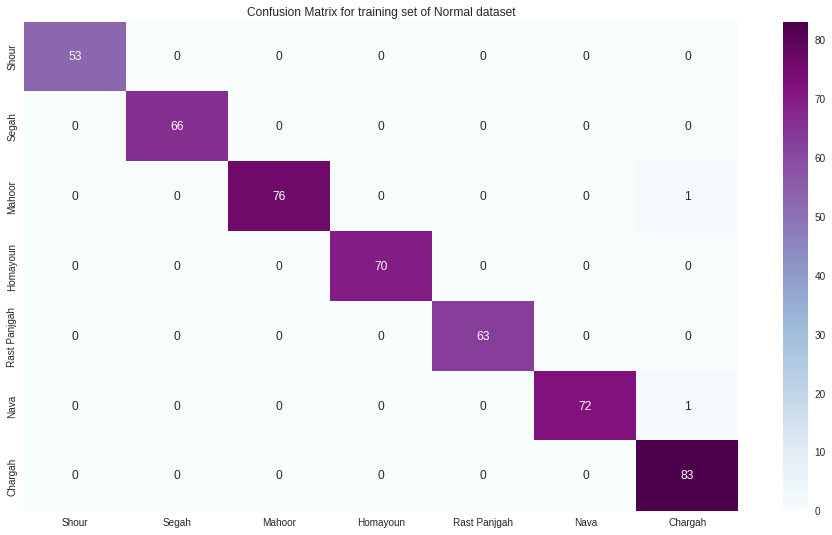
\includegraphics[width=0.7\linewidth]{Photo/40}
	\caption[نتایج \lr{Ensemble Learning} بر روی داده های train]{نتایج \lr{Ensemble Learning} بر روی داده های train}
	\label{fig:40}
\end{figure}
حال جدول نتایج به صورت زیر به دست می آید:\newline
\begin{table}[h]
	\centering
	\scalebox{0.8}{
		\begin{tabular}{l|l|l|l|l|}
			& \lr{precision} & \lr{recall} & \lr{f1-score} & \lr{support}  \\ 
			\hline
			شور          &$1$    & $1$   & $1$     &$53$       \\ 
			\hline
			سه گاه       & $1 $    &$1$  & $1   $  &$66$      \\ 
			\hline
			ماهور        &$ 1 $    & $0.987$  &$ 0.993$    &$ 77$      \\ 
			\hline
			همایون       &$1$     &$ 1$   &$1$    &$ 70 $      \\ 
			\hline
			راست پنج گاه &$1$   &$ 1$   &$ 1$     &$63$      \\ 
			\hline
			نوا          &$1$     &$ 0.986 $  &$ 0.993 $    & $73 $      \\ 
			\hline
			چهار گاه     &$ 0.976$      &$1$   & $0.988 $    &$ 83 $     \\ 
			\hline
			&           &        &          &          \\
			\lr{Accuracy}     &           &        &$ 0.996$     & $485$      \\ 
			\hline
			\lr{macro avg}    &$ 0.997    $   &$ 0.996 $   &$ 0.996 $    &$ 485  $    \\ 
			\hline
			\lr{weighted avg} & $0.996   $    & $0.996 $  & $0.996  $    & $485   $   \\
			\hline
	\end{tabular}}
	\caption{نتایج \lr{Ensemble Learning} بر روی داده های train} \label{foo15}
\end{table}





نتایج مدل ما بر داده ها نرمال test به صورت زیر به دست می آید:\newline
\begin{figure}[h]
	\centering
	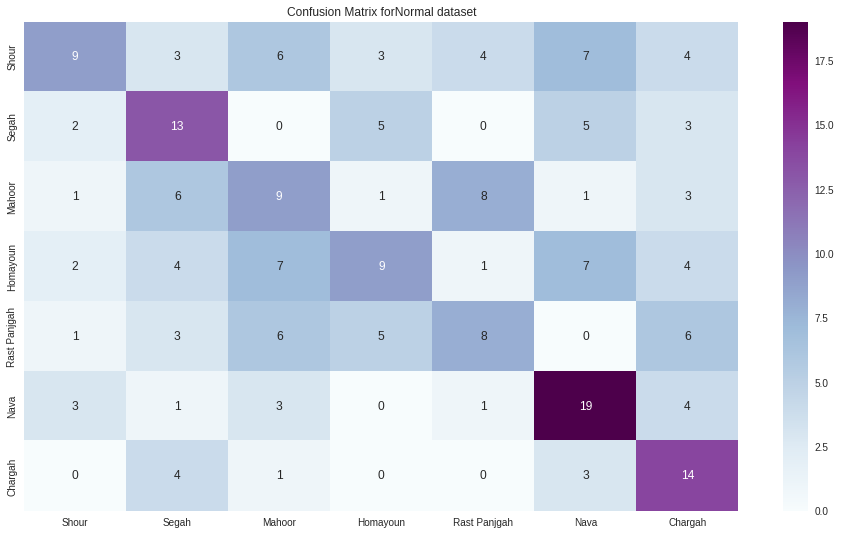
\includegraphics[width=0.7\linewidth]{Photo/41}
	\caption[نتایج \lr{Ensemble Learning} بر روی داده های test]{نتایج \lr{Ensemble Learning} بر روی داده های test}
	\label{fig:41}
\end{figure}
حال جدول نتایج به صورت زیر به دست می آید:\newline
\begin{table}[h]
	\centering
	\scalebox{0.8}{
		\begin{tabular}{l|l|l|l|l|}
			& \lr{precision} & \lr{recall} & \lr{f1-score} & \lr{support}  \\ 
			\hline
			شور          &$0.500$    & $0.25$   & $0.333$     &$36$       \\ 
			\hline
			سه گاه       & $0.382 $    &$ 0.464$  & $0.419   $  &$28$      \\ 
			\hline
			ماهور        &$ 0.281 $    & $0.310$  &$ 0.295$    &$ 29$      \\ 
			\hline
			همایون       &$ 0.391$     &$ 0.265$   &$ 0.316$    &$ 34 $      \\ 
			\hline
			راست پنج گاه &$ 0.364$   &$ 0.276$   &$ 0.314$     &$29$      \\ 
			\hline
			نوا          &$ 0.452$     &$ 0.613 $  &$ 0.521 $    & $31 $      \\ 
			\hline
			چهار گاه     &$ 0.368$      &$ 0.636$   & $0.467 $    &$ 22 $     \\ 
			\hline
			&           &        &          &          \\
			\lr{Accuracy}     &           &        &$ 0.388$     & $209$      \\ 
			\hline
			\lr{macro avg}    &$ 0.391    $   &$ 0.402 $   &$ 0.381 $    &$ 209  $    \\ 
			\hline
			\lr{weighted avg} & $0.396   $    & $0.388 $  & $0.376  $    & $209   $   \\
			\hline
	\end{tabular}}
	\caption{نتایج \lr{Ensemble Learning} بر روی داده های test} \label{foo16}
\end{table}




نتایج مدل ما بر داده ها غیر نرمال train به صورت زیر به دست می آید:\newline
\begin{figure}[h]
	\centering
	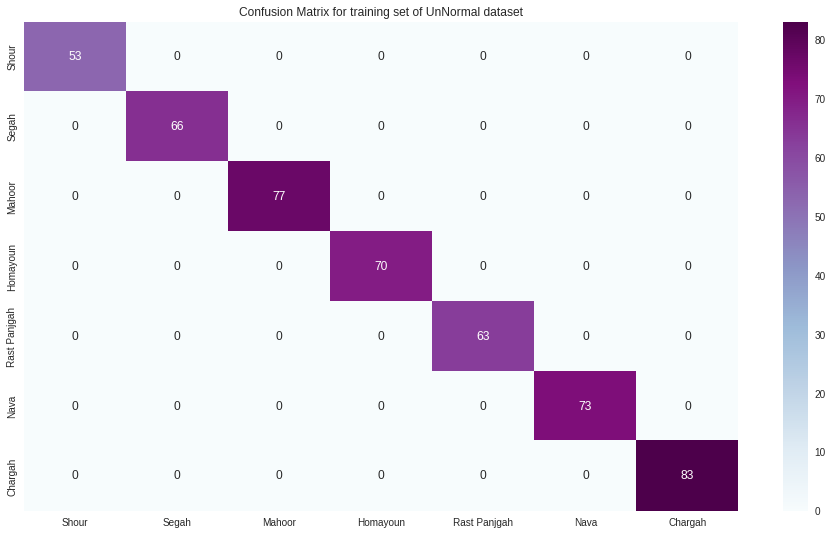
\includegraphics[width=0.7\linewidth]{Photo/42}
	\caption[نتایج \lr{Ensemble Learning} بر روی داده های غیر نرمال train]{نتایج \lr{Ensemble Learning} بر روی داده های غیر نرمال train}
	\label{fig:42}
\end{figure}

حال جدول نتایج به صورت زیر به دست می آید:\newline
\begin{table}[h]
	\centering
	\scalebox{0.8}{
		\begin{tabular}{l|l|l|l|l|}
			& \lr{precision} & \lr{recall} & \lr{f1-score} & \lr{support}  \\ 
			\hline
			شور          &$0.292$    & $0.269$   & $0.280$     &$26$       \\ 
			\hline
			سه گاه       & $0.312 $    &$ 0.370$  & $0.339   $  &$27$      \\ 
			\hline
			ماهور        &$ 0.407 $    & $0.306$  &$ 0.349$    &$ 36$      \\ 
			\hline
			همایون       &$ 0.368$     &$ 0.452$   &$ 0.406$    &$ 31 $      \\ 
			\hline
			راست پنج گاه &$ 0.273$   &$ 0.360$   &$ 0.310$     &$25$      \\ 
			\hline
			نوا          &$ 0.429$     &$ 0.316 $  &$ 0.364 $    & $38 $      \\ 
			\hline
			چهار گاه     &$ 0.407$      &$ 0.423$   & $0.415 $    &$ 26 $     \\ 
			\hline
			&           &        &          &          \\
			\lr{Accuracy}     &           &        &$ 0.354$     & $209$      \\ 
			\hline
			\lr{macro avg}    &$ 0.356    $   &$ 0.357 $   &$ 0.352 $    &$ 209  $    \\ 
			\hline
			\lr{weighted avg} & $0.363   $    & $0.354 $  & $0.354  $    & $209   $   \\
			\hline
	\end{tabular}}
	\caption{نتایج \lr{Ensemble Learning} بر روی داده های غیر نرمال train} \label{foo18}
\end{table}


نتایج مدل ما بر داده ها غیر نرمال train به صورت زیر به دست می آید:\newline
\begin{figure}[h]
	\centering
	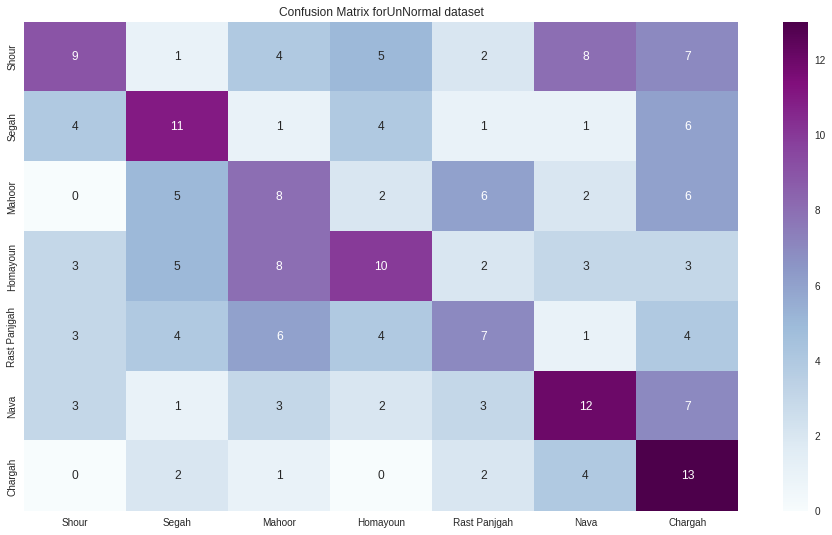
\includegraphics[width=0.7\linewidth]{Photo/43}
	\caption[نتایج \lr{Ensemble Learning} بر روی داده های غیر نرمال test]{نتایج \lr{Ensemble Learning} بر روی داده های غیر نرمال test}
	\label{fig:43}
\end{figure}

حال جدول نتایج به صورت زیر به دست می آید:\newline
\begin{table}[h]
	\centering
	\scalebox{0.9}{
		\begin{tabular}{l|l|l|l|l|}
			& \lr{precision} & \lr{recall} & \lr{f1-score} & \lr{support}  \\ 
			\hline
			شور          &$1$    & $1$   & $1$     &$65$       \\ 
			\hline
			سه گاه       & $1 $    &$ 1$  & $1   $  &$59$      \\ 
			\hline
			ماهور        &$ 1 $    & $1$  &$ 1$    &$ 78$      \\ 
			\hline
			همایون       &$ 1$     &$ 1$   &$ 1$    &$ 80 $      \\ 
			\hline
			راست پنج گاه &$ 1$   &$ 1$   &$ 1$     &$ 64$      \\ 
			\hline
			نوا          &$ 1$     &$ 1 $  &$ 1 $    & $73 $      \\ 
			\hline
			چهار گاه     &$ 1$      &$ 1$   & $1 $    &$ 71 $     \\ 
			\hline
			&           &        &          &          \\
			\lr{Accuracy}     &           &        &$ 1$     & $209$      \\ 
			\hline
			\lr{macro avg}    &$ 1    $   &$ 1 $   &$ 1 $    &$ 209  $    \\ 
			\hline
			\lr{weighted avg} & $1   $    & $1 $  & $1  $    & $209   $   \\
			\hline
	\end{tabular}}
	\caption{ نتایج \lr{Ensemble Learning} بر روی داده های غیر نرمال test} \label{foo19}
\end{table}


\subsection{۴-۶) \lr{XGboost}}
XGBoost يك طبقه بند از دستهي ensemble learning است كه به طور كلي از نركيب چندين و چند مدل ضعيفتر و قرار دادن آنها به صورت موازي يا سري به يك طبقهبند قويتر ميرسد. يك درخت تصميم كه واحدهاي سازندهي جنگلهاي تصادفي هستند در هر مرحله از عمقشان فضا را با استفاده از تنها يك ويژگي به دو قسمت تقسيم ميكنند و با عمق بيشتر افرازهاي بيشتر و قوانين طبقهبندي بيشتري را ايجاد ميكنند. درختهاي تصميم به دليل ساختار سادهي خود معمولا دقت پاييني دارند و نتيجهي خوبي در دنياي واقعي كسب نميكنند اما سازندگان الگوريتم ماشينلرنينگ با استفاده از اصل خرد جمعي)با رايگيري از تعداد افراد بسيار زياد خطا به نسبت كم ميشود( به اين نتيجه رسيدند كه هر بار درختها را با قسمت محدودي از ويژگيها آموزش دهند و در نهايت از بين تمام آنها رايگيري كنند. مشكل اصلي اين الگوريتم اين است كه درختها از اشتباهات يكديگر نميآموزند و عملا به درختها به صورت مستقل نگاه ميشود. روشهاي boosting براي حل اين مشكل به وجود آمدند. در روشهاي boosting درختها به جاي اين كه در توازي يكديگر باشند با يكديگر سري هستند و هر درخت روي خطاي درخت قبلي آموزش ميبيند. روشهاي مبتني بر گراديان به اين نحو عمل ميكنند كه درختهاي بعدي همجهت با تابع گراديان ويژگيهاي قبلي حركت ميكنند. Xgboost يك پيادهسازي موازي از الگوريتمهاي
مبتني بر گراديان است. ما در طبقهبندي خود از روش xgboost به دليل انعطاف بالاي آن در جذب اطلاعات استفاده
كرديم، كه به دليل تعداد دادههاي محدود پيشبيني ميشد كه مدل به دادههاي آموزش چسبنده شود كه نتايج اين نكته را تاييد ميكرد اما نكتهي بسيار قابل توجه اين است كه اين چسبندگي باعث عدم عموميتبخشي نشد و اين الگوريتم از تمام الگوريتمهاي ديگر بر روي دادهي ارزيابي عملكرد بهتري داشت. عكس هاي زير گفته هاي ما را تاييد ميكند، با توجه به اينكه -Cross Validation Score همواره با افزايش نمونه ها در حال افزايش است، ميتوان نتيجه گيري كرد كه مدل تشنه داده است. براي درك بهتر بايد مد نظر داشته باشيم دو منبع خطا به طور كلي وجود
دارد: الف( اشتباه در فرض اوليه براي مدل ب( كم بودن تعداد داده ها براي ابعاد مسئله حال با توجه به نمودار هاي شكل ۱۴ و دقتي كه براي مدل به دست آورديم مي توان نتيجه گرفت كه در مدل ساخته خطاي ”ب” جلوگيري ميكند از عملكرد بهتر مدل. در نهايت عملكرد مدل را نيز ميتوان مشاهده كرد به ازاي فيچر هاي مختلف:
با توجه نتايج مشاهده ميكنيم كه در دو كلاس لري و بندري با توجه به ريتيمي كه دارند خطاي كمتري وجود دارد اما در كلاس كردي،با توجه به اين نكته كه آهنگ هاي كردي از لحاظ ريتم و موسيقي همه طيف ها را در خود دارد در نتيجه بيشترين خطا را دارد. اما در مورد خطا متوجه ميشويم كه به داده هاي آموزش over fit شده است و براي حل مشكل دو راه وجود دارد، استفاده از مدل ساده تر و افزايش نمونه ها. در نمودار cross val score و توضيحات آن گفته شد
كه اضافه كردن داده به مدل ميتواند راه حل مناسب تري باشد.\newline
حال مدل ما بر روی داده های نرمال train به صورت زیر خواهد بود:\newline
\begin{figure}[h]
	\centering
	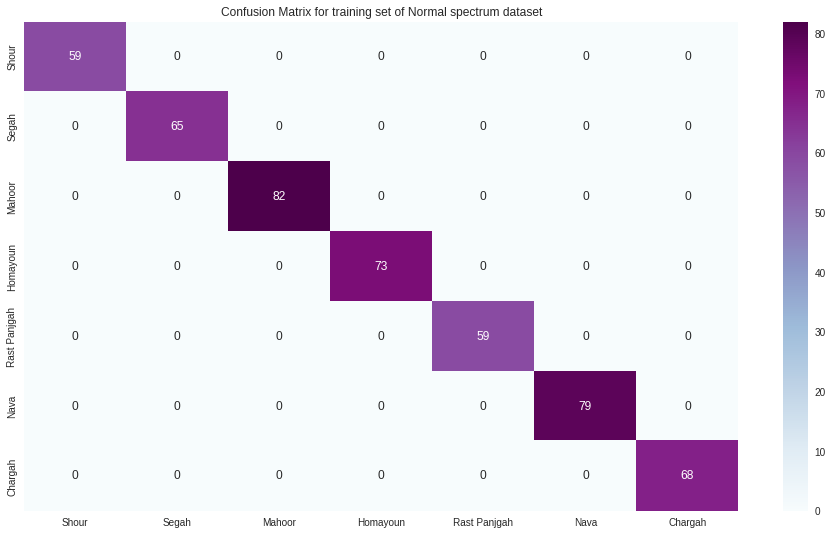
\includegraphics[width=0.7\linewidth]{Photo/44}
	\caption[نتایج \lr{XGboost} بر روی داده های غیر نرمال train]{نتایج \lr{XGboost} بر روی داده های غیر نرمال train}
	\label{fig:45}
\end{figure}
 و جدول آن به صورت زیر خواهد بود:\newline
 \begin{table}[h]
 	\centering
 	\scalebox{0.9}{
 		\begin{tabular}{l|l|l|l|l|}
 			& \lr{precision} & \lr{recall} & \lr{f1-score} & \lr{support}  \\ 
 			\hline
 			شور          &$1$    & $1$   & $1$     &$65$       \\ 
 			\hline
 			سه گاه       & $1 $    &$ 1$  & $1   $  &$59$      \\ 
 			\hline
 			ماهور        &$ 1 $    & $1$  &$ 1$    &$ 78$      \\ 
 			\hline
 			همایون       &$ 1$     &$ 1$   &$ 1$    &$ 80 $      \\ 
 			\hline
 			راست پنج گاه &$ 1$   &$ 1$   &$ 1$     &$ 64$      \\ 
 			\hline
 			نوا          &$ 1$     &$ 1 $  &$ 1 $    & $73 $      \\ 
 			\hline
 			چهار گاه     &$ 1$      &$ 1$   & $1 $    &$ 71 $     \\ 
 			\hline
 			&           &        &          &          \\
 			\lr{Accuracy}     &           &        &$ 1$     & $485$      \\ 
 			\hline
 			\lr{macro avg}    &$ 1    $   &$ 1 $   &$ 1 $    &$ 485  $    \\ 
 			\hline
 			\lr{weighted avg} & $1   $    & $1 $  & $1  $    & $485   $   \\
 			\hline
 	\end{tabular}}
 	\caption{ نتایج \lr{XGboost} بر روی داده های غیر نرمال test} \label{foo20}
 \end{table}


در ادامه مدل ما بر روی داده های نرمال test به صورت زیر خواهد بود:\newline
\begin{figure}[h]
	\centering
	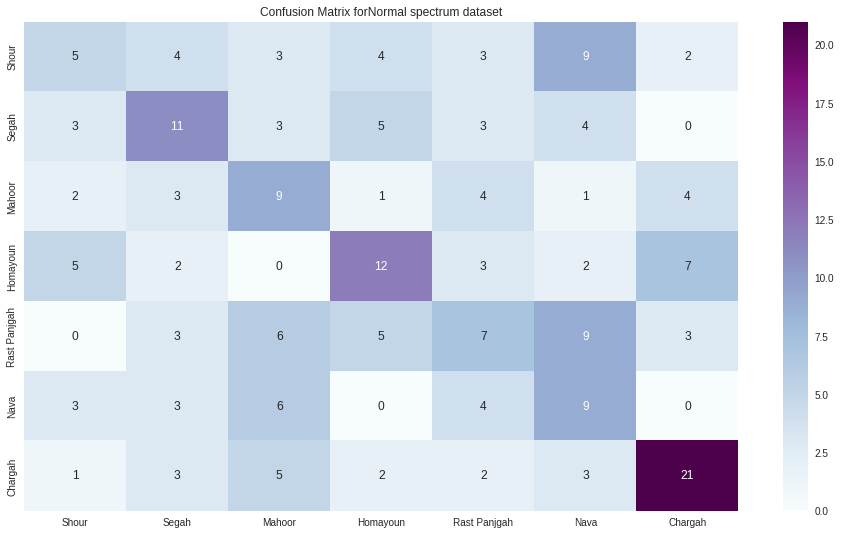
\includegraphics[width=0.7\linewidth]{Photo/45}
	\caption[نتایج \lr{XGboost} بر روی داده های غیر نرمال test]{نتایج \lr{XGboost} بر روی داده های غیر نرمال test}
	\label{fig:44}
\end{figure}
\subsection{۴-۷) مقایسه}
 داده‌ها پیچیده بودن این نوع داده, همانطور که پیشبینی می‌شد مدل‌هایی مانند SVM خطی و به طور کلی مدل‌های ساده, دقت نسبتا پایینی برای طبقه‌بندی می‌دهند. بهترین مدل در این بخش مدل شبکه‌ی عصبی بود که مشخص است با توجه به اینکه این مدل قابلیت استخراج روابط پیچیده است قابل پیش‌بینی بود.
همچنین شایان ذکر است که در تمام مدل‌ها استفاده از داده‌ی نورمال نشده, باعث بدتر شدن مدل‌ها می‌شود.
\section{۵) خوشه بندی}
خوشه‌بندی یا به عبارتی \lr{Clustring} وظیفه گروه‌بندی مجموعه‌ای از اشیاء است به گونه‌ای که اشیاء در یک گروه (به نام خوشه) شباهت بیشتری به یکدیگر داشته باشند تا در گروه‌های دیگر و به طورکلی با روش های مختلف داده ها به خوشه های مختلف تقسیم می شوند.\newline

\subsection{۵-۱) K-means}
به طورکلی در \lr{K-means} هدف این است که مرکزهایی را انتخاب کند که اینرسی، یا مجموع مربعات درون خوشه را به حداقل برساند.
\begin{equation}
	\sum_{i=0}^{n}\min_{\mu_j \in C}(||x_i - \mu_j||^2)
\end{equation}
اینرسی را می توان به عنوان معیاری برای میزان انسجام درونی خوشه ها درنظر گرفت. از معایب مختلفی تاثیر می پذیرد: \newline
۱) اینرسی این فرض را ایجاد می کند که خوشه ها محدب و همسانگرد هستند، که همیشه اینطور نیست. به خوشه های دراز یا منیفولدهایی با اشکال نامنظم واکنش ضعیفی نشان می دهد. \newline
۲) اینرسی یک متریک نرمال شده نیست: ما فقط می دانیم که مقادیر کمتر بهتر است و صفر بهینه خواهد بود. اما در فضاهای با ابعاد بسیار بالا، فواصل اقلیدسی تمایل دارند که متورم شوند (این نمونه ای از به اصطلاح "نفرین ابعاد" است). اجرای یک الگوریتم کاهش ابعاد مانند تجزیه و تحلیل مؤلفه اصلی (PCA) قبل از خوشه بندی k-means می تواند این مشکل را کاهش دهد و محاسبات را سرعت بخشد. \newline
در پیاده سازی \lr{K-means} سه مرحله دارد:\newline
-اولین مرحله، مرکزهای اولیه را انتخاب می‌کند، با اساسی‌ترین روش، انتخاب K نمونه از مجموعه داده‌ها\newline
-پس از مقداردهی اولیه، K-means شامل حلقه زدن بین دو مرحله دیگر است.\newline
۱) مرحله اول هر نمونه را به نزدیکترین مرکز خود اختصاص می دهد.\newline
۲) مرحله دوم با در نظر گرفتن مقدار میانگین تمام نمونه های اختصاص داده شده به هر مرکز قبلی، مرکزهای جدید ایجاد می کند. تفاوت بین مرکز قدیمی و جدید محاسبه می شود و الگوریتم این دو مرحله آخر را تا زمانی که این مقدار کمتر از یک آستانه باشد تکرار می کند. به عبارت دیگر، آنقدر تکرار می شود که مرکزها حرکت قابل توجهی نداشته باشند.\newline
\begin{figure}[h]
	\centering
	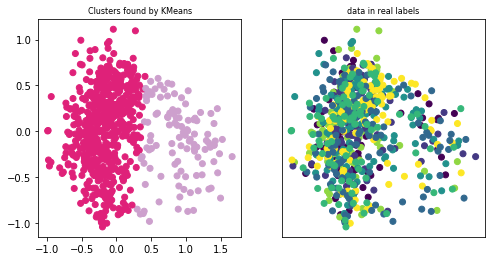
\includegraphics[width=0.5\linewidth]{Photo/download2}
	\caption[دسته بندی های مختلف با kmeans]{دسته بندی های مختلف با kmeans}
	\label{fig:download2}
\end{figure}
\begin{figure}[h]
	\centering
	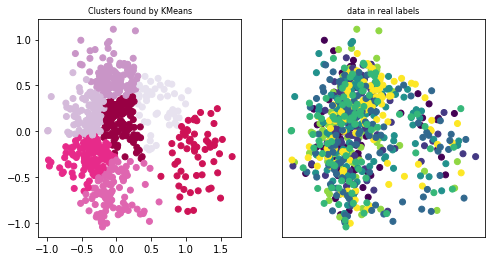
\includegraphics[width=0.5\linewidth]{Photo/download}
	\caption[دسته بندی های مختلف با kmeans]{دسته بندی های مختلف با kmeans}
	\label{fig:download}
\end{figure}
\begin{figure}[h]
	\centering
	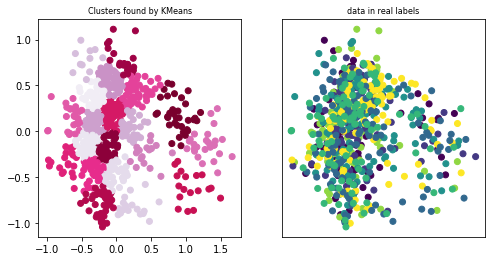
\includegraphics[width=0.5\linewidth]{Photo/download1}
	\caption[دسته بندی های مختلف با kmeans]{دسته بندی های مختلف با kmeans}
	\label{fig:download1}
\end{figure}
برای راحتی درک این خوشه‌بندی برای دوتا از PCAها مهمتر را نیز جدا کرده‌ایم و شکل زیر را رسم کردیم.  مشخص است که داده‌ها به سادگی جدایی‌پذیر نیستند و خوشه‌بندی برای حالات ۲ و ۵ و ۷ به شکل زیر می‌باشد:


حال با توجه به ماتریس‌های درهمریختگی موارد زیر را می‌توان استنتاج کرد:
\begin{itemize}
	\item با توجه به کلاس‌بندی دو کلاسه فرضیه ما راحع به به سادگی جداپذیر نبودن داده‌ها تایید می‌شود. یعنی مشخص است که بیشتر داده‌ها در یک خوشه‌ قرار گرفته‌اند. 
		\item کلاس‌بندی ۷ کلاسه نیز تا حد زیادی داده‌ها به صورت تصادفی پخش شده‌اند, این قضیه نیز با توجه به ماهیت داده‌ها قابل توجیه است زیرا که با توجه به توزیع داده‌ها و شبیه بودن این داده‌ها به هم, مشخص است که خوشه‌بندی در بعد فعلی امکان‌پذیر نبوده و نتایج صحیح می‌باشد.
		\item باتوجه به خوشه بندی ۲۱ تایی همان طور که انتظار می رفت داده ها به صورت تصادفی پخش شده اند این قضیه با توجه به این که توضیع داده ها بسیار شبیه به هم بود در بعد فعلی جدایی پذیر نیست قابل توجیه است. همچنین ماتریس آشفتگی می توان از شباهت بین کلاس و خوشه ها پی برد برای مثال بیشتر داده های کلاس پنج در خوشه هفتم قرار گرفته است همچنین تعداد زیادی از داده های کلاس یک, دو , سه و هفت در یک خوشه قرار گرفته‌اند  که به معنی شبیه بودن این کلاس‌ها به یکدگیر است.
\end{itemize}
\begin{figure}[h]
	\centering
	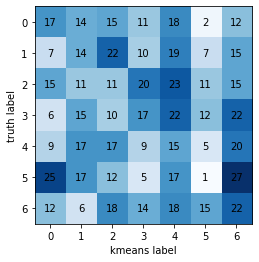
\includegraphics[width=0.7\linewidth]{Photo/37}
	\caption[خوشه بندی \lr{K-means}]{خوشه بندی \lr{K-means}}
	\label{fig:37}
\end{figure}

البته باید دقت داشت تعداد خوشه‌های مناسب باید با استفاده از روش زانویی سنجیده شود. با توجه به نمودار زانویی رسم شده, نیز می‌توان فهمید بهترین تعداد خوشه ۷ تا است که به تعداد کلاس‌هایمان می‌باشد.
\begin{figure}[h]
	\centering
	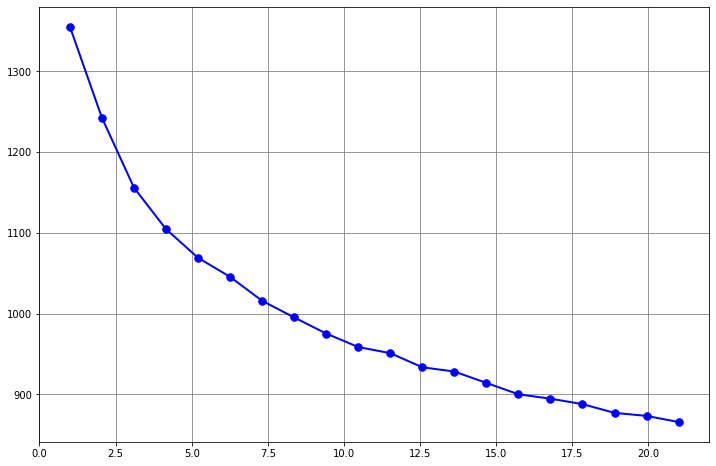
\includegraphics[width=0.7\linewidth]{Photo/38}
	\caption[نمودار زانویی \ \lr{K-means}]{نمودار زانویی \lr{K-means}}
	\label{fig:38}
\end{figure}

\subsection{۵-۲) \lr{Spectral Clustering}}
خوشه‌بندی طیفی را می‌توان به‌عنوان خوشه‌بندی نموداری در نظر گرفت. برای داده های مکانی می توان به القای یک نمودار بر اساس فواصل بین نقاط (به طور بالقوه یک نمودار k-NN یا حتی یک نمودار متراکم) فکر کرد. از آنجا، خوشه‌بندی طیفی به بردارهای ویژه لاپلاسین گراف نگاه می‌کند تا تلاش کند یک جاسازی خوب (بعد پایین) نموداری در فضای اقلیدسی پیدا کند. این اساساً نوعی یادگیری چندگانه است، یافتن دگرگونی فضای اصلی به گونه‌ای است که فاصله‌های چندگانه را برای چند منیفولی که داده‌ها فرض می‌شود در نظر می گیرد، بهتر نشان دهد. هنگامی که فضای تبدیل شده را داشته باشیم، یک الگوریتم خوشه بندی استاندارد اجرا می شود. با 'sklearn' پیش فرض K-Means است. این بدان معناست که کلید خوشه بندی Spectral، دگرگونی فضا است. با فرض اینکه بهتر بتوانیم manifold را اجرا کنیم، خوشه بندی بهتری به دست خواهیم آورد.
\begin{figure}[h]
	\centering
	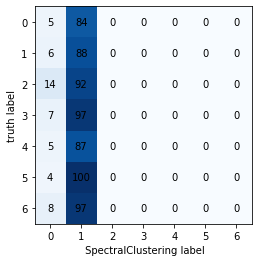
\includegraphics[width=0.7\linewidth]{Photo/SC1}
	\caption[ماتریس پاکندگی spectral]{ماتریس پاکندگی spectral}
	\label{fig:sc1}
\end{figure}
\begin{figure}[h]
	\centering
	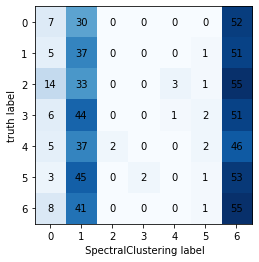
\includegraphics[width=0.7\linewidth]{Photo/SC}
	\caption[ماتریس پاکندگی spectral]{ماتریس پاکندگی spectral}
	\label{fig:sc}
\end{figure}
\begin{figure}[h]
	\centering
	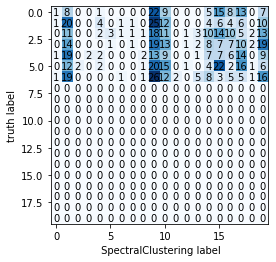
\includegraphics[width=0.7\linewidth]{Photo/SC2}
	\caption[ماتریس پاکندگی spectral]{ماتریس پاکندگی spectral}
	\label{fig:sc2}
\end{figure}
ما نیاز به نگرانی کمتری در مورد خوشه های کروی K-Means داریم، زیرا آنها فقط در فضای تبدیل شده کروی هستند و نه فضای اصلی. ما متأسفانه برخی از نقاط ضعف K-Means را حفظ می کنیم: ما همچنان داده ها را به جای خوشه بندی آن ها تقسیم بندی می کنیم. حدس زدن پارامتر "تعداد خوشه ها" سخت است. ما مشکلات پایداری داریم که از K-Means به ارث رسیده است. بدتر از آن، اگر بر روی نمودار متراکم ماتریس فاصله عمل کنیم، گام اولیه بسیار گرانی خواهیم داشت و عملکرد را قربانی می کنیم.

\begin{figure}[h]
	\centering
	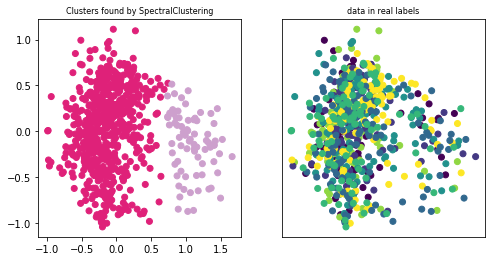
\includegraphics[width=0.7\linewidth]{Photo/SC3}
	\caption[خوشه بندی spectral]{خوشه بندی spectral}
	\label{fig:sc3}
\end{figure}
\begin{figure}[h]
	\centering
	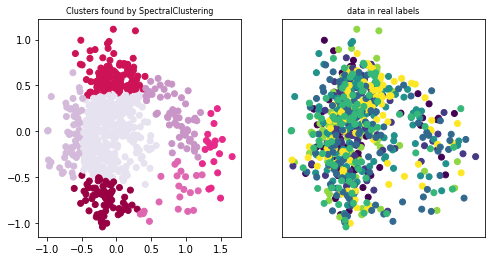
\includegraphics[width=0.7\linewidth]{Photo/SC4}
	\caption[خوشه بندی spectral]{خوشه بندیی spectral}
	\label{fig:sc4}
\end{figure}
\begin{figure}[h]
	\centering
	\includegraphics[width=0.7\linewidth]{Photo/SC5}
	\caption[خوشه بندی spectral]{خوشه بندی spectral}
	\label{fig:sc5}
\end{figure}
درکل می توان گفت که باتوجه به این روش به این که این روش تمرکز زیادی رو نقاط اطراف دارد و نزدیک بودن مقادیر ویژگی ها در این روش به هم, اکثر داده ها در یک کلاس قرار گرفته و باتوجه به این موضوع روش مناسبی نخواهد بود.و البته می توان باتوحه به ماتریس در هم ریختگی گفت که داده ها چگال هستند با فاصله زیاد از هم و در دو خوشه دسته بندی می شوند.
\section{۶) نتیجه گیری}
مقایسه بین مدل‌ها و نتیجه‌گیری\newline
مقایسه کلی \newline
با توجه به نوع داده‌ها و اینکه داده‌های صوتی به سادگی جدایی‌پذیر نیست، دقت پایین اکثر مدل‌ها توجیه‌پذیر می‌باشد. بهترین مدل‌ها برای اینکار مدل‌هایی بود که می‌توانست داده را به فضایی دیگر تصویر کند و در فضای جدید داده‌ها را طبقه‌بندی کند. برای مثال طبقه‌بندهای MLP و SVM RBF بهترین نتیجه‌ها را در مقایسه با سایر مدل‌ها می‌دهند. شایان به ذکر است که همانطور که در بخش‌های قبلی ییشنهاد شد، برای داده‌های صوتی بهتر است از مدل‌های حافظه‌دار مانند LSTM استفاده شود. همچنین در مواردی مانند  
نورمالایز شده و نشده\newline
نرمال‌سازی یک تکنیک مقیاس‌پذیری در یادگیری ماشینی است که در طول آماده‌سازی داده‌ها برای تغییر مقادیر ستون‌های عددی در مجموعه داده به منظور استفاده از یک مقیاس مشترک استفاده می‌شود. برای همه مجموعه داده ها در یک مدل ضروری نیست. تنها زمانی مورد نیاز است که ویژگی‌های مدل‌های یادگیری ماشین دارای محدوده‌های متفاوتی باشند. برای داده‌های ما با توجه به اینکه جنس ویژگی‌ها مختلف بوده، و همچنین در رنج‌های مختلف قرار دارند لازم است که حتما نورمالیزیشن صورت بگیرد.\newline
نورمال کردن داده‌ها در اکثر موارد باعث بهتر شدن نتیجه نهایی همه‌ی مدل‌ها می‌شود. البته در بعضی از مدل‌ها مانند XGBoost به صورت built-in این موضوع پیاده‌سازی شده است. با مقایسه دقت و ماتریس‌های درهمریختگی مدل‌های مختلف لزوم نورمالایزیشن واضح است.\newline


\section{۷)  ضمیمه}
کد‌های ‌پیاده‌سازی به صورت فایل‌های نوت‌بوک در کنار این پروژه پیوست شده‌اند. در فایل \lr{Feature extraction} ابتدا, ویژگی‌های مختلف فایل‌های صوتی به نمایش درآمده‌اند. همچنین, ویژگی‌های مختلفی استخراج شده‌اند و در فایل‌های csv قرار گرفته‌اند. در این پروژه دو دسته ویژگی برای کارهای خوشه‌بندی و طبقه‌بندی در نظر گرفته شده است که هرکدام در فایل‌های کد متناسب نتایج آن قابل مشاهده است. \newline
همچنین برای داده‌های نورمالایز شده, نورمالایز نشده و حالت کاهش ویژگی در فایل‌های مختلف عملیات‌های لازم انجام شده‌ است و قابل مقایسه است.
عملیات‌های طبقه‌بندی در فایل‌هایی با نام \lr{Classification} قرار گرفته‌اند. همچنین عملیات‌های خوشه‌بندی در فایل‌هایی با نام clustering قرار گرفته‌اند.
\begin{figure}[h]
	\centering
	\includegraphics[width=0.7\linewidth]{Photo/f1}
	\caption[نرمالایز شده و نشده]{نرمالایز شده و نشده}
	\label{fig:f1}
\end{figure}

کاهش ویژگی\newline
کاهش وِیژگی با استفاده از روش‌های انتخاب ویژگی معمولا منجر به بدتر شدن طبقه‌بندهای ما می‌شود. این موضوع به این دلیل است که ویژگی‌های استخراج شده هیچکدام به تنهایی قابلیت توجیه داده‌ها را ندارند. همچنین شایان به ذکر است که در مواردی مانند PCA این روش سعی دارد ویژگی‌هایی را نگه دارد که بیشترین واریانس را در آن‌ها داریم، لذا با توجه به اینکه این واریانس را می‌توان به نویز نیز نسبت داد. در شرایطی که داده‌های ما سیگنال صوتی هستند کاهش ویژگی می‌تواند باعث بدتر شدن نتیجه‌ی نهایی شود.\newline
\begin{figure}[h]
	\centering
	\includegraphics[width=0.7\linewidth]{Photo/LDAsvm}
	\caption[LDA برای svm]{LDA برای svm}
	\label{fig:ldasvm}
\end{figure}
\begin{figure}[h]
	\centering
	\includegraphics[width=0.7\linewidth]{Photo/PCAsvm}
	\caption[PCA برای svm]{PCA برای svm}
	\label{fig:pcasvm}
\end{figure}

ویژگی‌های مختلف\newline
ما دو دسته از ویژگی‌های mel-spectogram در کنار mfcc و chroma برای آموزش مدل‌ها استفاده کرده‌ایم. ویژگی spectrogram به طور کلی نتیجه‌ی بدتری نسبت به دیگر ویژگی به ما می‌داد. البته این موضوع با توجه به ماهیت این ویژگی قابل بیان بود. برای هر کدام از این ویژگی‌های roc آن نمایش داده شده است که کامل‌ها آن‌ها در کد قابل رویت است.\newline
خوشه‌بندی\newline
الگوریتم خوشه‌بندی kmeans با توجه به اینکه داده‌ها، در حالت عادی بسیار نزدیک به هم هستند قابلیت جداسازی مناسبی ندارد، اما با توجه به این الگوریتم، شباهت بین داده‌ها را می‌توانیم مشاهده کنیم.


\end{document}
